\documentclass{report}

\usepackage[T1]{fontenc}
\usepackage[ngerman]{babel}
\usepackage[utf8]{inputenc}
\usepackage{lmodern}

\usepackage{amsmath}
\usepackage{amsthm}
\usepackage{amssymb}
\usepackage{physics}

\usepackage{graphicx}

\usepackage[colorlinks]{hyperref}

% Randbreite reduzieren
\usepackage[paper=a4paper, left=25mm, right=25mm, top=25mm, bottom=25mm]{geometry}

% Entfernt das Einrücken von Absätzen 
\usepackage{parskip}

\usepackage{siunitx}

\title{Moderne Physik: Vorlesungs- und Übungs-Mitschrieb}
\author{Daniel Seemaier, Christoph Michelbach}
\date{\today}

\makeatletter
\hypersetup{
    colorlinks,
    citecolor=black,
    filecolor=black,
    linkcolor=blue,
    urlcolor=black,
    pdftitle={\@title},
    pdfauthor={\@author},
    bookmarks=true
}

\newcommand{\mdotvec}[1]{\dot{\vec{#1}}}
\newcommand{\mddotvec}[1]{\ddot{\vec{#1}}}
\newcommand{\msimplediff}[2]{\frac{\mathrm{d}#1}{\mathrm{d}#2}}
\newcommand{\mnorm}[1]{\left\lVert #1 \right\rVert}
\newcommand{\mabs}[1]{\left\lvert #1 \right\rvert}
\newcommand{\mvec}[1]{\begin{pmatrix} #1 \end{pmatrix}}
\newcommand{\md}{\mathrm{d}}
\newcommand{\mset}[1]{\left\{ #1 \right\}}
\newcommand{\mimpuls}[1]{\ensuremath{p_#1}}
\newcommand{\mpoison}[2]{\ensuremath{\{ #1, \, #2 \}}}
\newcommand{\dint}{\mathrm{d}} % d beim Ableiten und Integrieren

\begin{document}
	\maketitle

	\setcounter{chapter}{-1}
	\chapter{Einleitung}

Verstehen im Gegensatz zur "`klassischen Physik"', entwickelt ab Anfang des 20. Jhd. Wichtigste Entwicklungen im 1. Viertel des Jhd.

Bis dahin (grob vereinfacht):
\begin{itemize}
	\item Newtonsche Mechanik
	\item Maxwells Elektrodynamik
\end{itemize}

\textbf{Paradigma}: alles im Prinzip berechenbar (Zeitentwicklung von System), solange die Anfangsbedingungen (alle $\vec{x}_i(t_0)$, $\dot{\vec{x}}_i(t_0)$, wobei $i =$ alle Punkte) bekannt sind.

\textbf{Aber}: Experimente zeigen immer mehr Widersprüche, zum Beispiel:
\begin{itemize}
	\item Michelson-Morley-Experiment: es gibt keinen "`Äther"', daraus hat sich die Spezielle Relativitätstheorie von Einstein (SRT) entwickelt
	\item Diskrete Energiespektren (Spektrallinien)
	\item Welleneigenschaft von Teilchen
	\item Teilcheneigenschaften von Lichtwellen
	\item Schwarzkörperstrahlung
	\item[$\Rightarrow$] das führte zur Quantenphysik 
\end{itemize}

Aufbau der Vorlesung:
\begin{enumerate}
	\item Klassische Mechanik
	\begin{itemize}
		\item Newtonsche Mechanik (sehr kurz)
		\begin{itemize}
			\item Entwicklung der formaleren analytischen Mechanik (Lagrange, Hamilton, Jacobi)
			\item erlaubt theoretische Diskussionen, z.B. Symmetrien und Erhaltungssätze; andere Konzepte, die in der Quantenmechanik (QM) eine Rolle spielen; "`Hamiltonoperator"'; kanonisch konjugierte Variable
		\end{itemize}
	\end{itemize}
	
	\item Relativität
	\begin{itemize}
		\item Symmetrie von Raum und Zeit
		\begin{itemize}
			\item daraus die Spezielle Relativität entwickeln (etwas losgelöst von klassischer Mechanik)
			\item formale Entwicklung, dann radikale Konsequenzen bestimmen
		\end{itemize}
	\end{itemize}
	
	\item Quantenmechanik
	\begin{itemize}
		\item wenig (?) Historie
		\item einfache eindimensionale Probleme 
		\begin{itemize}
			\item Schrödingergleichung
			\item Zusammenhang zur Wellenmechanik
		\end{itemize}
		\item Postulate der Quantenmechanik
		\item Symmetrien (?)
		\item Wasserstoffatom (System der Elemente)
		\item Identische Teilchen 
		\item Beispiele \dots
	\end{itemize}
\end{enumerate}
	\chapter{Klassische Mechanik}

\section{Abriss der Newtonschen Mechanik}

Problemstellung der klassischen Mechanik: Orte $\vec{r}_i$ und Geschwindigkeiten $\vec{v}_i$ zur Zeit $t$ gegeben für ein System von Massenpunkten mit $1 \le i \le N$ (also $N$ Massenpunkte).

Es wirken äußere Kräfte $\vec{F}$ und Kräfte zwischen den Teilchen $i$ und $j$ ($i \neq j$): $\vec{F}_{ij}$.

Wie lauten die \textbf{kinematischen Größen} $\vec{r}_i(t)$ und $\vec{v}_i(t) = \mdotvec{r}_i(t)$ (wobei $\mdotvec{r} = \msimplediff{\vec{r}}{t}$) für beliebige Zeiten $t$ danach?

Die kinematischen Größen $\vec{r}_i(t)$ (und $\mdotvec{r}_i(t)$) werden als Lösungen gewöhnlicher Differentialgleichungen gefunden; das sind die \textbf{Bewegungsgleichungen}.

Neben diesen kinematischen Größen gibt es die wichtigen Begriffe \textbf{Kraft}, \textbf{Masse}, \textbf{Impuls} und \textbf{Energie}.


\textbf{Kraft}: vektorielle Größe, meistens $\vec{F}$ (manchmal auch $\vec{K}$); ist immer die Ursache von Bewegung oder der Änderung von Bewegungszuständen, das heißt im Umkehrschluss: kräftefrei $\rightarrow$ Bewegung unverändert 
	
Das führt auf die \textbf{Newtonschen Gesetze}: 
\begin{description}
	\item[lex prima (Galileisches Trägheitsgesetz)] es gibt Initialsysteme, in denen ein kräftefreier Körper (= Massepunkt) ruht oder sich gradlinig gleichförmig bewegt
		
	\textbf{Definition}: Jeder Massepunkt setzt der Einwirkung von Kräften einen \textbf{Trägheitswiderstand} entgegen = Masse, oder besser: \textbf{träge Masse} (Formelzeichen: $m$)
		
	\textbf{Definition}: \textbf{Impuls} $\vec{p} = m \vec{v}$
		
	\item[lex secunda (Bewegungsgesetz)] $\mdotvec{p} = \vec{F}$; meistens ist $m$ unveränderlich, dann ist $\mdotvec{v} = \msimplediff{}{t} \vec{v} = \vec{a}$ und $\vec{F} = m \vec{a}$.
		
	\item[lex tertia (actio = reactio)] $\vec{F}_{ij} = - \vec{F}_{ji}$ 
	
	\begin{figure}
		\centering
		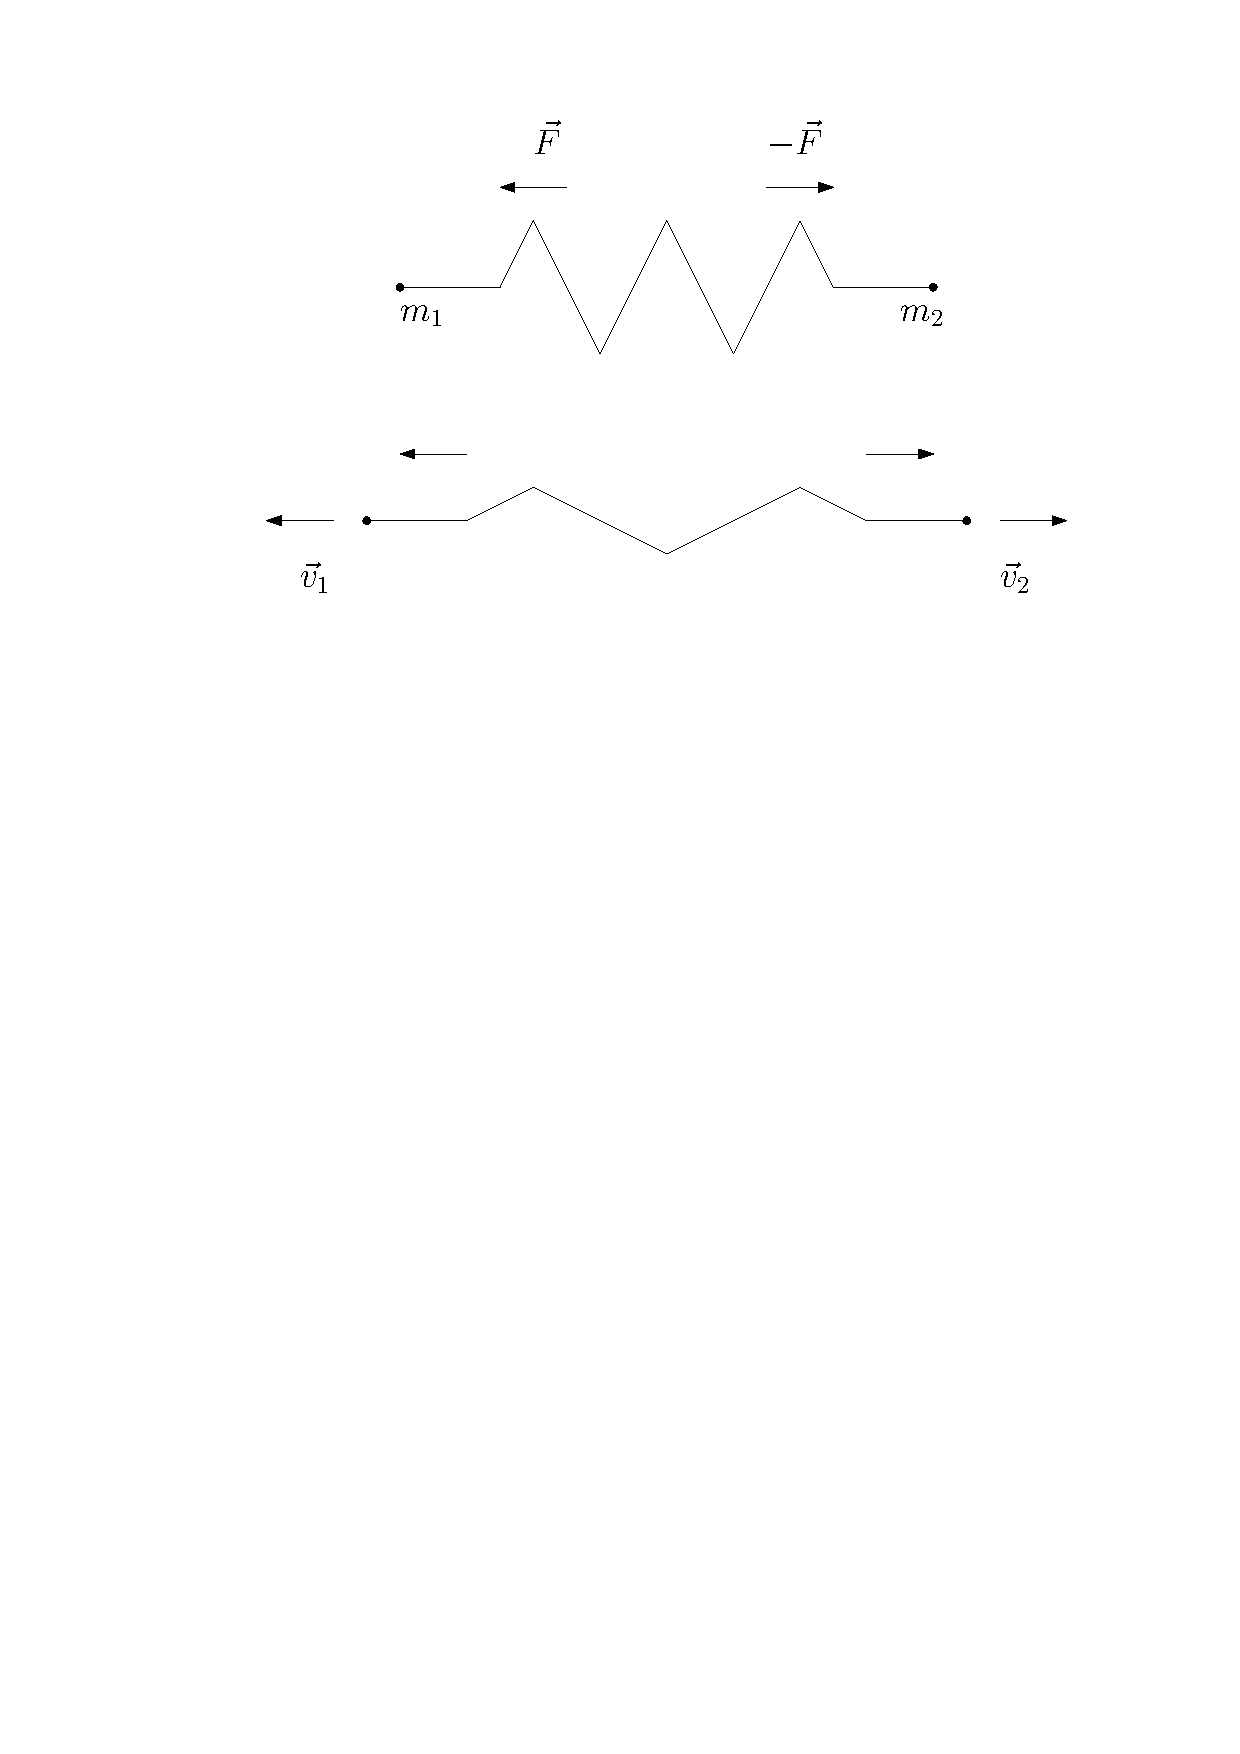
\includegraphics[scale=0.5]{figures/ch1/feder}
		\caption{actio = reactio bei einer Feder}
		\label{fig:ch1_feder}
	\end{figure}

	
	Beobachtung aus Abbildung \ref{fig:ch1_feder}: $\frac{v_1}{v_2} = \frac{m_2}{m_1}$, unabhängig von $\vec{F}$; das führt auf die Massendefinition
\end{description}

Wichtige Beispiele für Kräfte:

\begin{description}
	\item[Gravitationskraft (schwere Masse = träge Masse)] $\vec{F} = -\gamma \frac{M m}{r^2} \hat{r}$, wobei $\hat{r} = \frac{\vec{r}}{\mabs{\vec{r}}}$ und $\gamma$ die Gravitationskonstante ist
	
		Skizze
	
		Speziell auf der Erde: $r = r_e$, $M = M_e$, $\gamma$
		
		Damit $F = \underbrace{\gamma \frac{M_e}{r_e^2}}_{=: g} m = mg$ und $g \approx 9.81 m s^{-2}$; die Kraft zeigt nach unten, deswegen nur noch $F$ statt $\vec{F}$
	\item[Coloumbkraft] $\vec{F} = \frac{1}{4 \pi \epsilon_0} \frac{Q_1 Q_2}{r^2} \hat{r}$ zwischen elektrischen Ladungen $Q_1$ und $Q_2$; das sind zwei Zentralkräfte.
	\item[Lorentzkraft] $\vec{F} = e (\vec{E} + \vec{v} \times \vec{B})$: Ladung $e$, elektrisches Feld $\vec{E}$ und magnetisches Feld $\vec{B}$.
	\item[harmonischer Oszillator] lineare, stets negative (bezüglich der Bewegung) Kraft: $F = -\alpha \mabs{x}$
\end{description}

\textbf{Intertialsysteme / Nichtinertialsyseme}: In einem Inertialsystem: kräftefrei = gleichförmige Bewegung. 

Systeme $\Sigma$, $\Sigma'$ sind vollkommen gleichwertig, d.h. die physikalischen Gesetze sind forminvariant (kovariant) unter sogenannten Galilei-Transformationen. Das sind solche, die aus $\vec{r}' = \vec{r} + \vec{v}_0t$ machen, wenn sich $\Sigma$ und $\Sigma'$ mit $\vec{v}_0$ (=const) relativ zueinander bewegen. 

In \textbf{beschleunigten Systemen} gibt es sogenannte \textbf{Scheinkräfte};  zum Beispiel in rotierenden Systemen (Zentrifugalkraft, Corioliskraft).

Weitere Themen:
\begin{itemize}
	\item Schwingungsysteme (mit Dämpfung)
	\item Mehrere Massenpunkte (Eigenschwingungen)
	\item viel mehr Massenpunkte, "`starre Körper"'; Bewegung von Schwerpunkt + Rotation = "`Kreiselbewegung"'
\end{itemize}

\section{Lagrange-Mechanik}

Ausgangspunkt: Newton $m \mddotvec{r} = \vec{F}_i + \sum^N_{j \neq i} \vec{F}_{ij}$ für $i, j = 1, \dots, N$. $\vec{F}_i$ ist eine externe Kraft, $\vec{F}_{ij}$ sind Kräfte zwischen beteiligten Teilchen, paarweise. Damit: Problem vollständig formuliert, denn das sind $3N$ gewöhnliche Differentialgleichungen 2. Ordnung. Die sind im Prinzip lösbar mit den entsprechenden Anfangsbedingungen.

\textbf{Probleme}: 
\begin{itemize}
	\item Formulierung in Koordinaten $(x, y, z)_i$ ist meist zu kompliziert; damit wird die Lösung hoffnungslos.
	\item Meist Probleme mit eingeschränkter Geometrie. Zum Beispiel Perle auf kreisförmigem Draht (siehe Abbildung \ref{fig:ch1_perleaufdraht}). $(x, y, z)$ der Perle sinnvoll? $\phi$ viel geeigneter.
	\begin{figure}
		\centering
		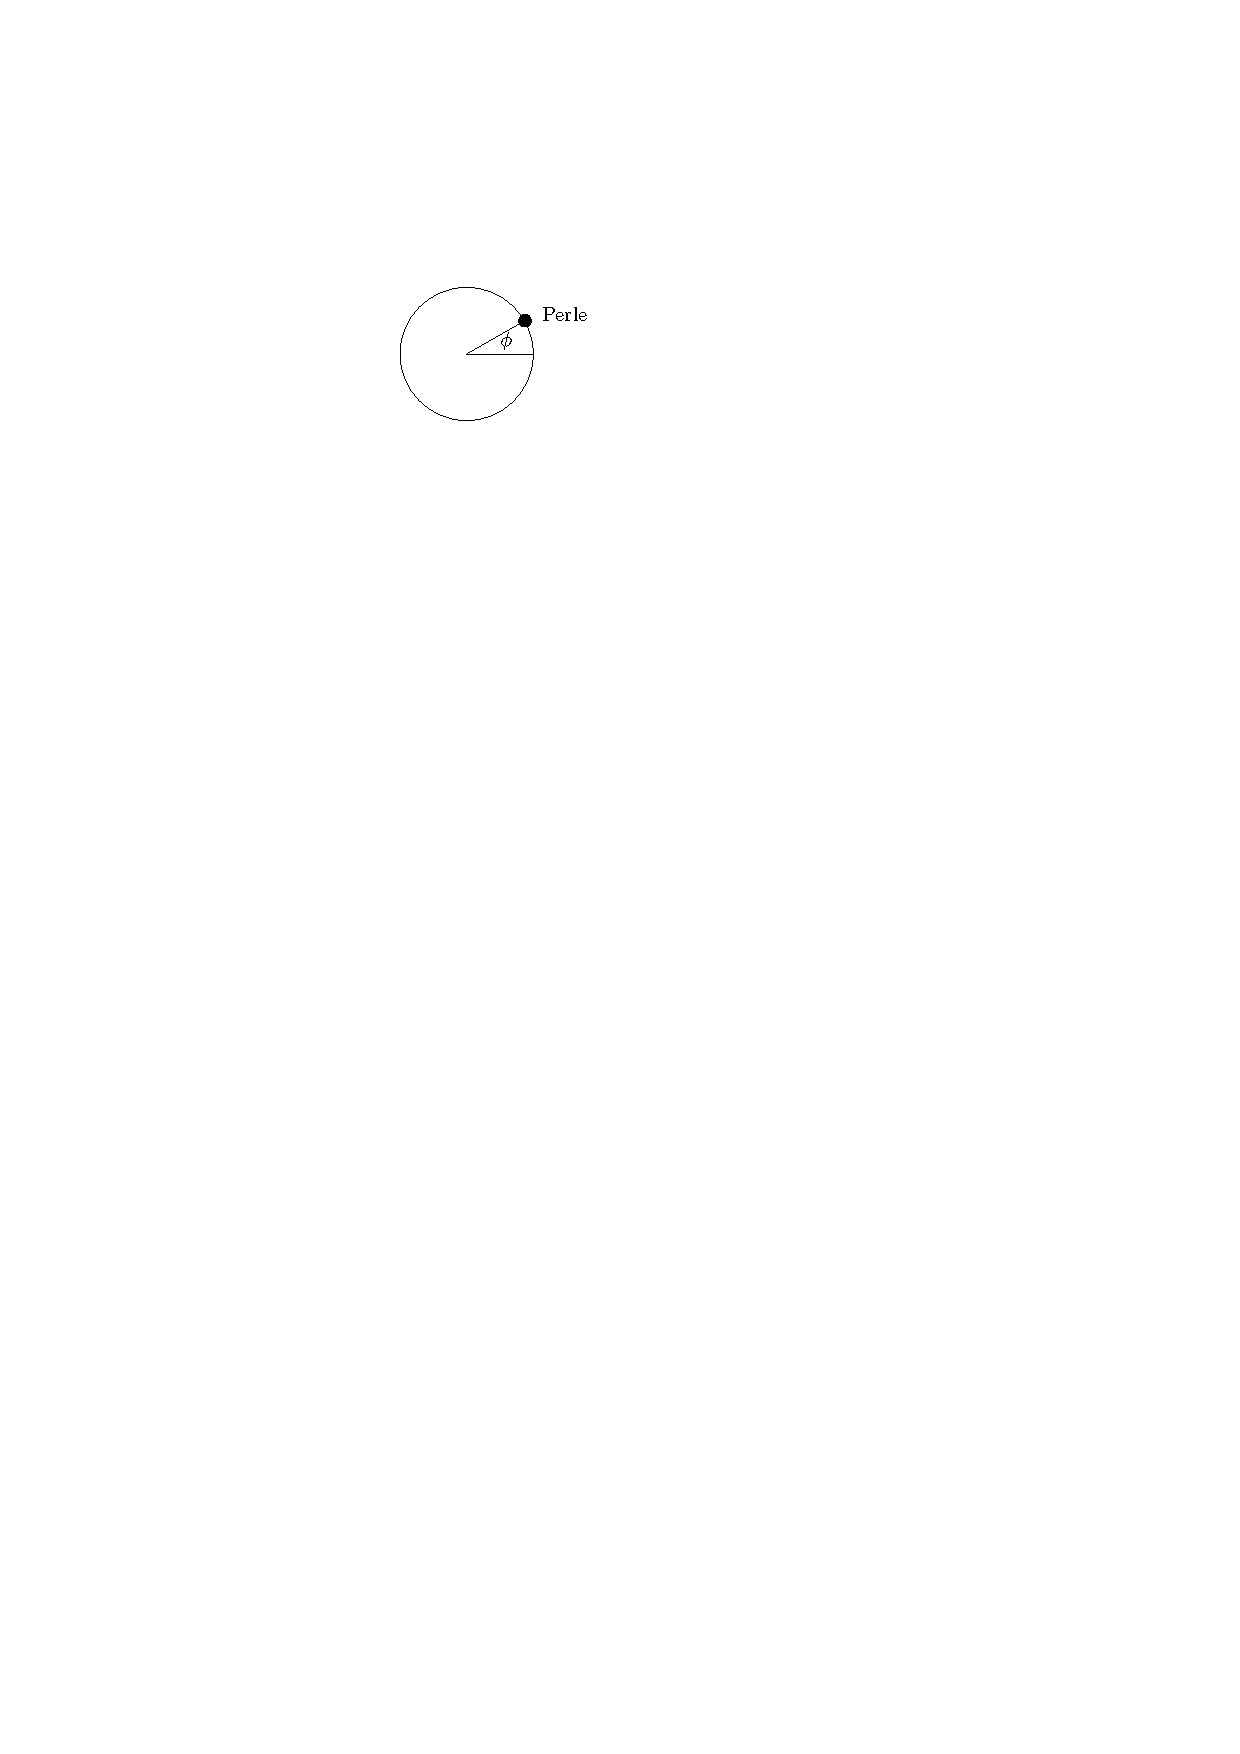
\includegraphics{figures/ch1/perleaufdraht}
		\caption{Die Position der Perle mit $\phi$ auszudrücken ist sinnvoller als mit $(x, y, z)$}
		\label{fig:ch1_perleaufdraht}
	\end{figure}
\end{itemize}

Die $\vec{F}_{ij}$ beschreiben geometrische Beziehungen auf komplizierte Weise $\rightarrow$ \textbf{Zwangskräfte} (im Beispiel die Kräfte, die die Perle auf dem Draht halten). Diese bewirken \textbf{Zwangsbedingungen}, die eigentlich direkt viel einfacher zu formulieren sind.

\textbf{Ziel der Lagrange-Mechanik}: Elimination der Zwangskräfte per verallgemeinerter Koordinaten (meist weniger als vorher)

Zwangsbedingungen sind:
\begin{itemize}
	\item A
	\begin{itemize}
		\item A1: holonom-shleronom(?): $\frac{\partial f_\nu}{\partial t} = 0$ mit $\nu = 1, \dots, p$ 
		\item A2: holonom-rheonom: $\frac{\partial f_\nu}{\partial t} \neq 0$ mit $\nu = 1, \dots, p$
	\end{itemize}
	\item B
	\begin{itemize}
		\item B1: als Ungleichungen $\rightarrow$ keine elimin... Bedingungen
		\item B2: differentielle Form: ???
	\end{itemize}
\end{itemize}


\textbf{Beispiele}:
\begin{itemize}
	\item Hantel (A1; siehe Abbildung \ref{fig:ch1_hantel}): $f(\vec{r}_i, \vec{r}_2) = 0$ und $(x_1 - x_2)^2 + (y_1 - y_2)^2 + (z_1 - z_2)^2 - l^2 = 0$.
	\begin{figure}
		\centering
		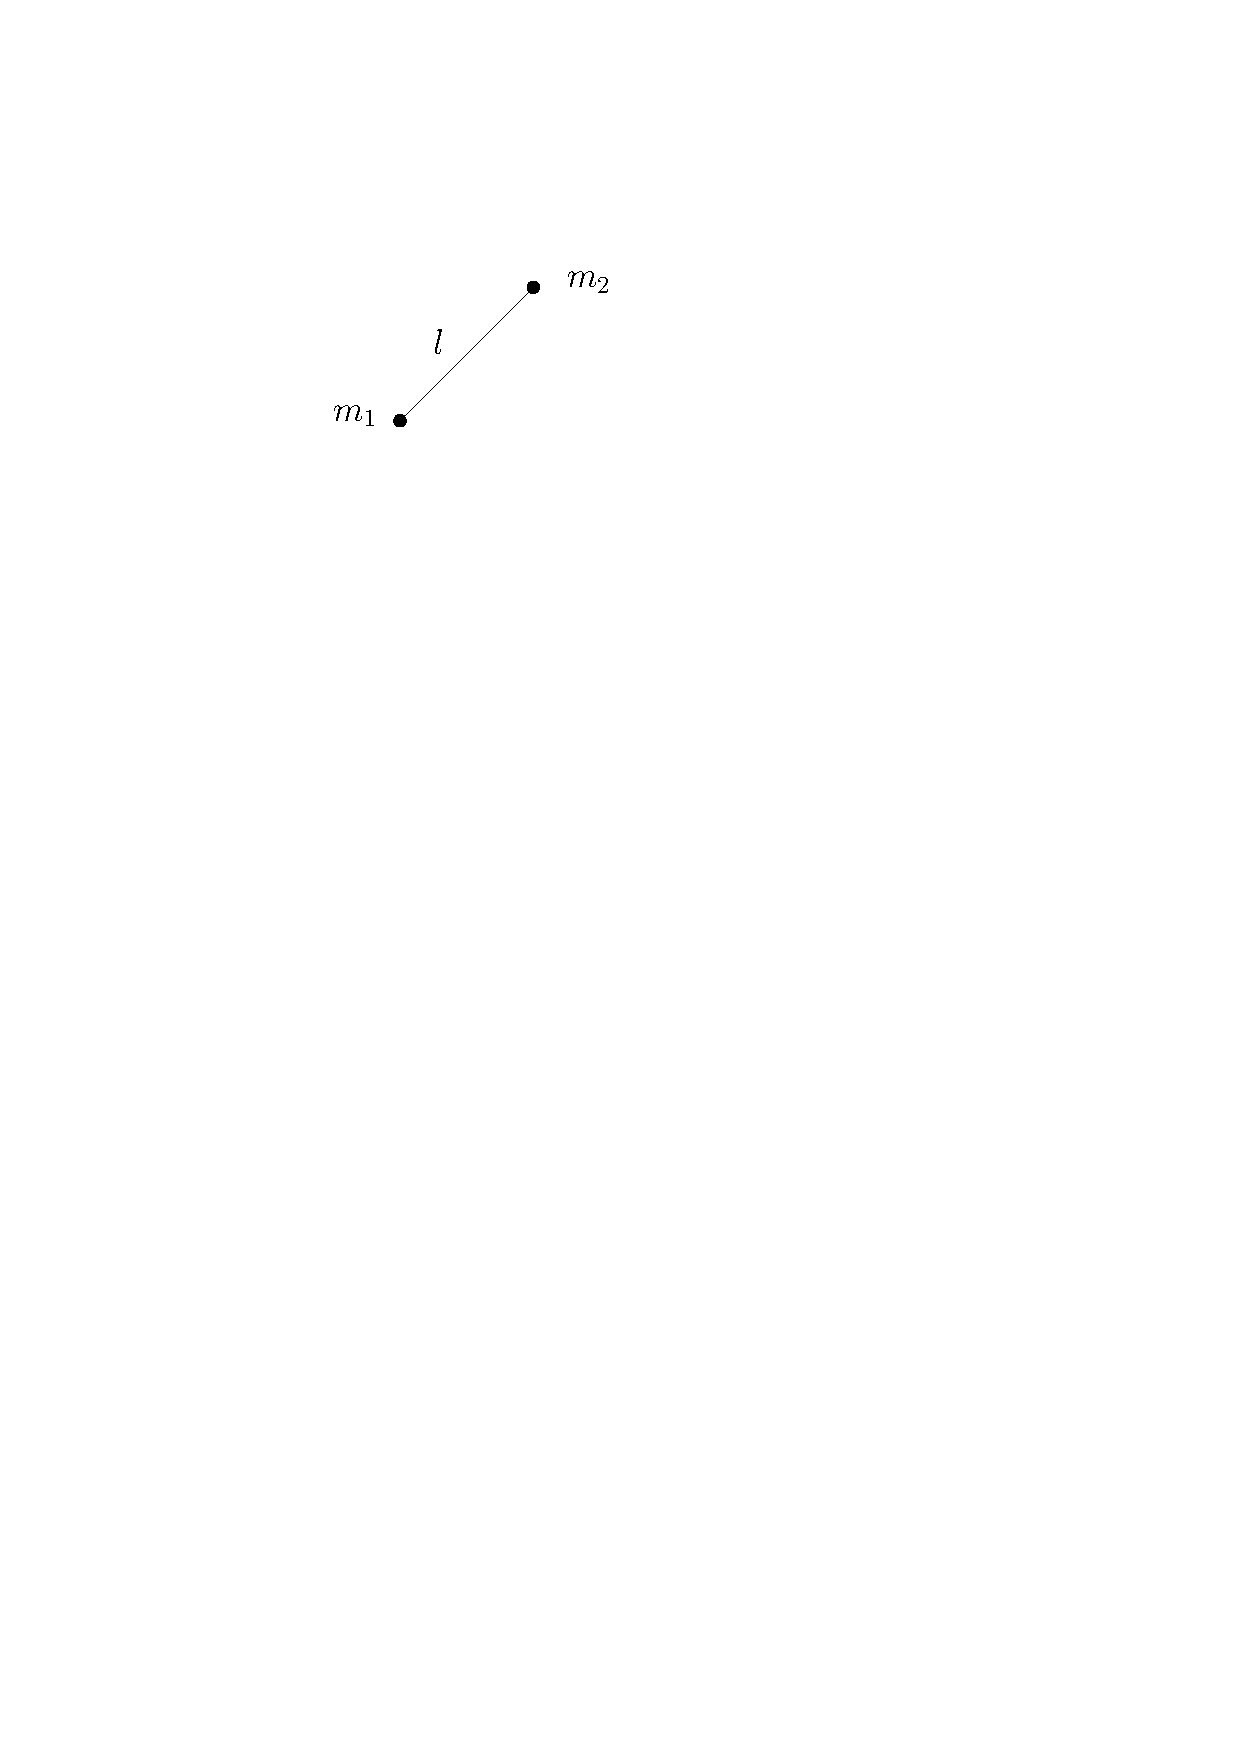
\includegraphics{figures/ch1/hantel}
		\caption{Eine Hantel der Länge $l$.}
		\label{fig:ch1_hantel}
	\end{figure}
	
	\item Ebene mit variablem Winkel (A2; siehe Abbildung \ref{fig:ch1_schiefeebene}): $\frac{z}{x} = \tan \phi(t)$
	\begin{figure}
		\centering
		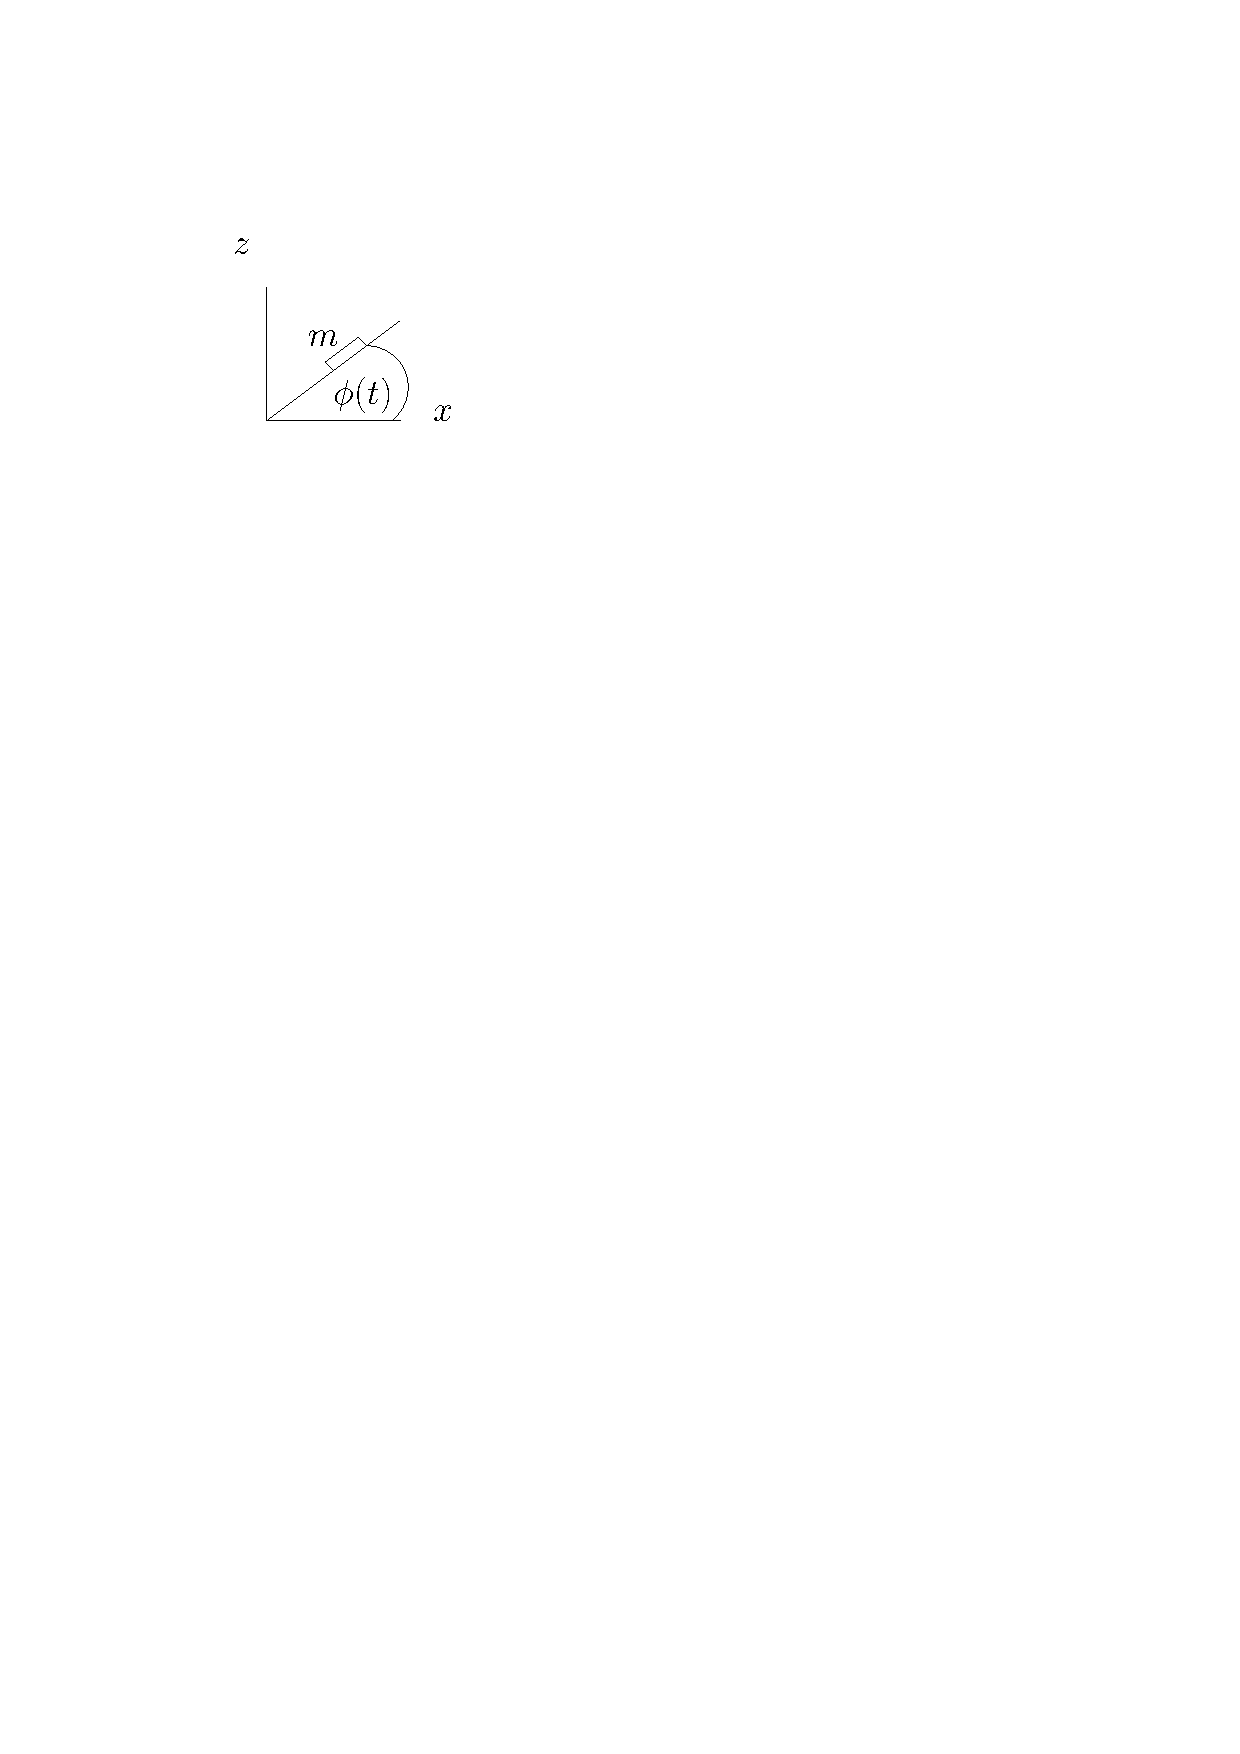
\includegraphics{figures/ch1/schiefeebene}
		\caption{Eine Hantel der Länge $l$.}
		\label{fig:ch1_schiefeebene}
	\end{figure}
\end{itemize}

Holonom: Reduktion der Freiheitsgrade $S = 3N - p$ bei $p$ holonomen Zwangsbedingungen $\rightarrow$ generalisierte Koordinaten, genannt $q_1, \dots, q_S$. Mit $\vec{r}_i = \vec{r}_i(q_1, \dots, q_S, t)$ sind Zwangsbedingungen implizit. Es gibt \textbf{keine} Beziehung $f(q_1, \dots, q_S, t) = 0$, d.h. es können keine Koordinaten eliminiert werden; $q_i$ unabhängig!

Schreibe $\vec{q} = (q_1, \dots, q_S)$ = Vektor aus dem $S$-dimensionalen Konfigurationsraum. Weiter sind $\dot{q}_1, \dots, \dot{q}_S$ die generalisierten Geschwindigkeiten.

\textbf{Bemerkung}: 
\begin{itemize}
	\item Mit $\vec{q}_0$, $\mdotvec{q}_0$ als Anfangsbedingungen sollte der Zustand zu jeder Zeit danach (oder davor) zu bestimmen sein.
	\item $\mset{q_S}$ ist nicht eindeutig, wohl aber die Anzahl $S$ (ergibt sich aus der physikalischen Problemstellung).
	\item Die $q_i$ haben eine nicht vorgegebene Dimension (müssen keine Längen sein, können z.B. auch Winkel sein). Eventuell ist die physikalische Bedeutung der $q_i$ nicht offensichtlich. Meistens sind es aber geometrische Größe.
\end{itemize}

\textbf{Beispiele}:
\begin{enumerate}
	\item Teilchen auf einer Kugeloberfläche (siehe Abbildung \ref{fig:ch1_kugel}) $\vec{r} = (x, y, z)$; $p = 1$ 
	
	\textbf{Zwangsbedingung}: $x^2 + y^2 + z^2 - R^2 = 0$, also $S = 3 - 1 = 2$. 
	
	$2$ quadratische Koordinaten, z.b. Winkel $q_1 = \nu$, $q_2 = \phi$
	\begin{figure}
		\centering
		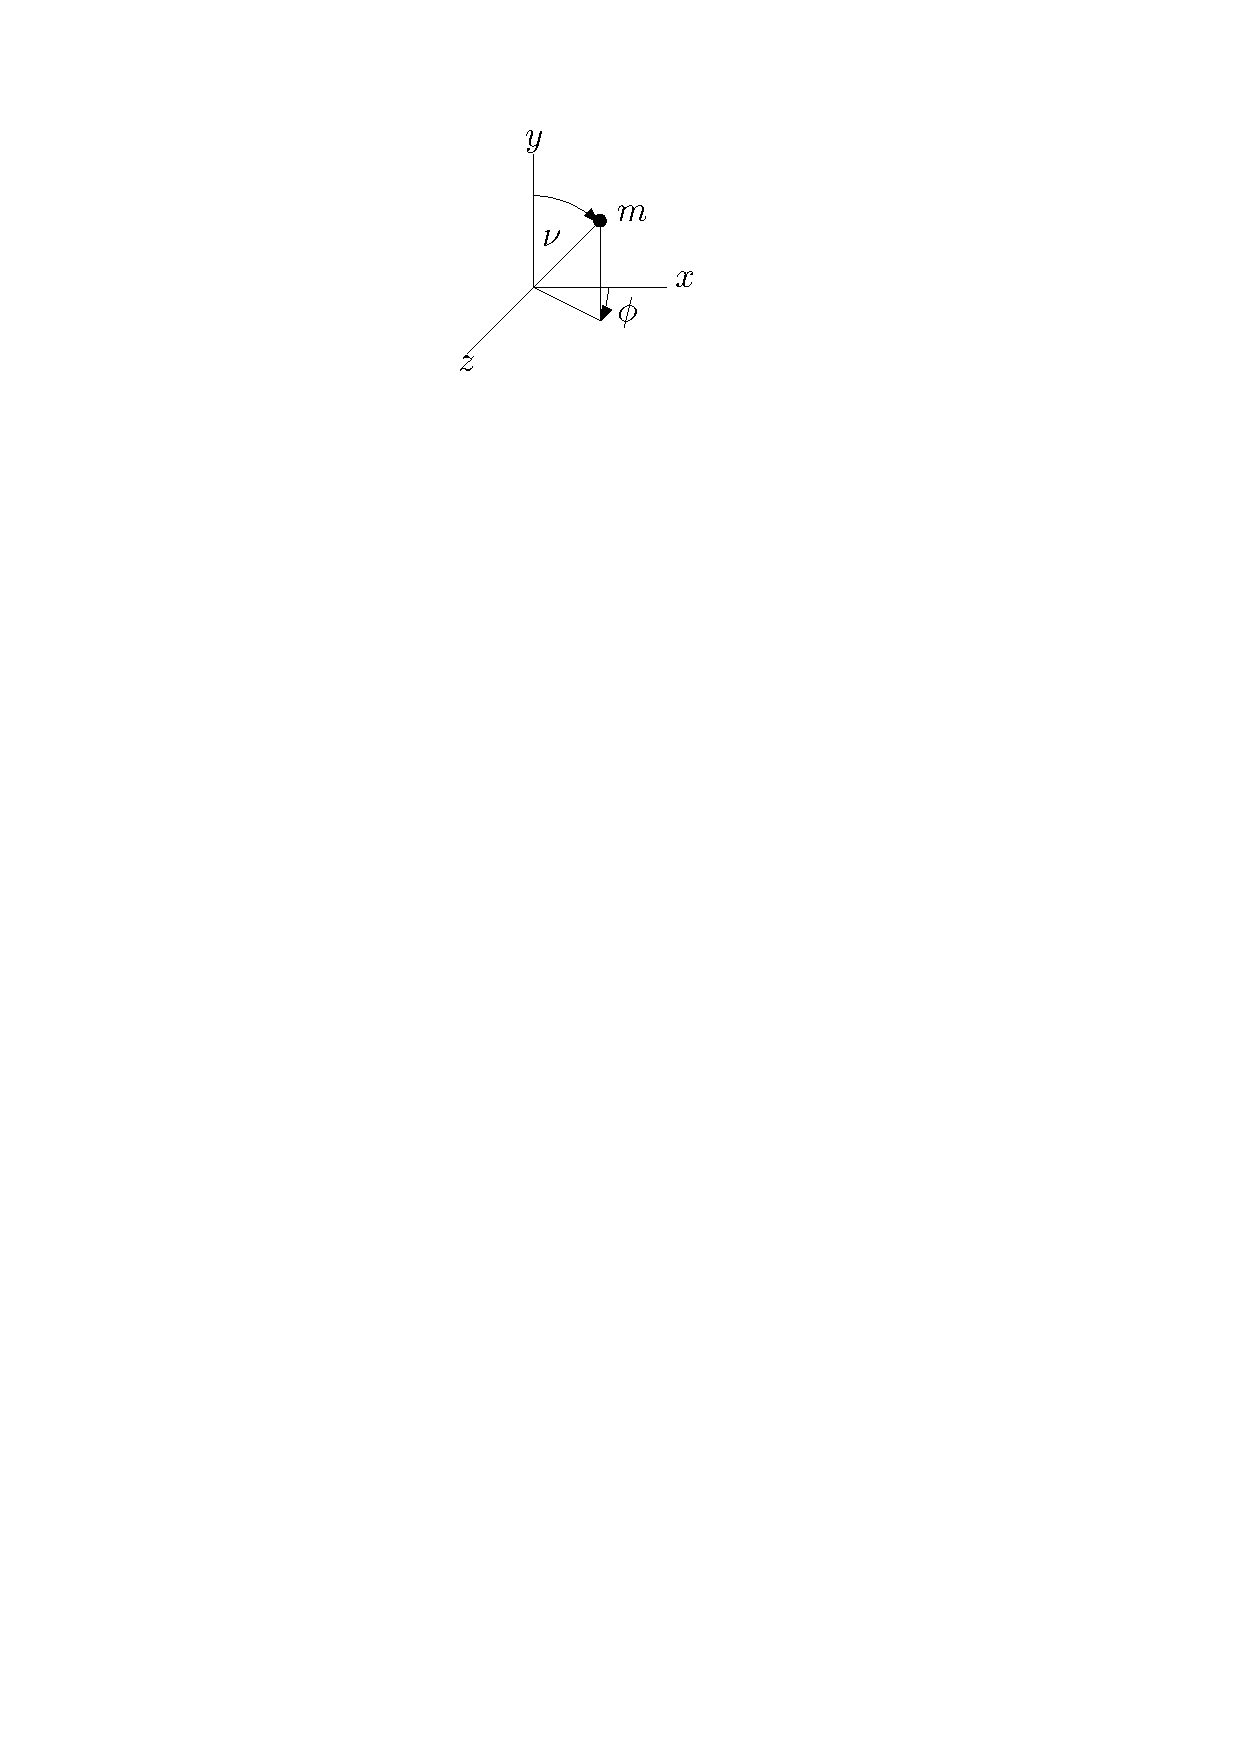
\includegraphics{figures/ch1/kugel}
		\caption{Kugel}
		\label{fig:ch1_kugel}
	\end{figure}
	
	$x = R \sin q_1 \cos q_2$, $y = R \sin q_1 \sin q_2$, $z = R \cos q_1$ $\rightarrow$ Zwangsbedingungen sind implizit, denn bei dieser Beschreibung immer erfüllt
	
	\item Doppelpendel (siehe Abbildung \ref{fig:ch1_doppelpendel}): zwei Massen $m_1$, $m_2$ = $6$ Freiheitsgrade
	
	vier davon sind holonom-shleronom: $z_1 = z_2 = ?$, $x_1^2 + y_1^2 - l_1^2 = 0$, $(x_2 - x_1)^2 + (y_2 - y_1)^2 - l_2^2 = 0$
	
	Wie viel generalisierte Koordinaten? $S = 6 - 4 = 2$ $\rightarrow$ zum Beispiel $q_1 = \nu_1$, $q_2 = \nu_2$
	
	$x_1 = l_1 \cos q_1$, $y_1 = l_1 \sin q_1$, $z_1 = 0$
	
	$x_2 = l_1 \cos q_1 + l_2 \cos q_2$, $y_2 = l_1 \sin q_1 + l_2 \sin q_2$, $z_2 = 0$
	\begin{figure}
		\centering
		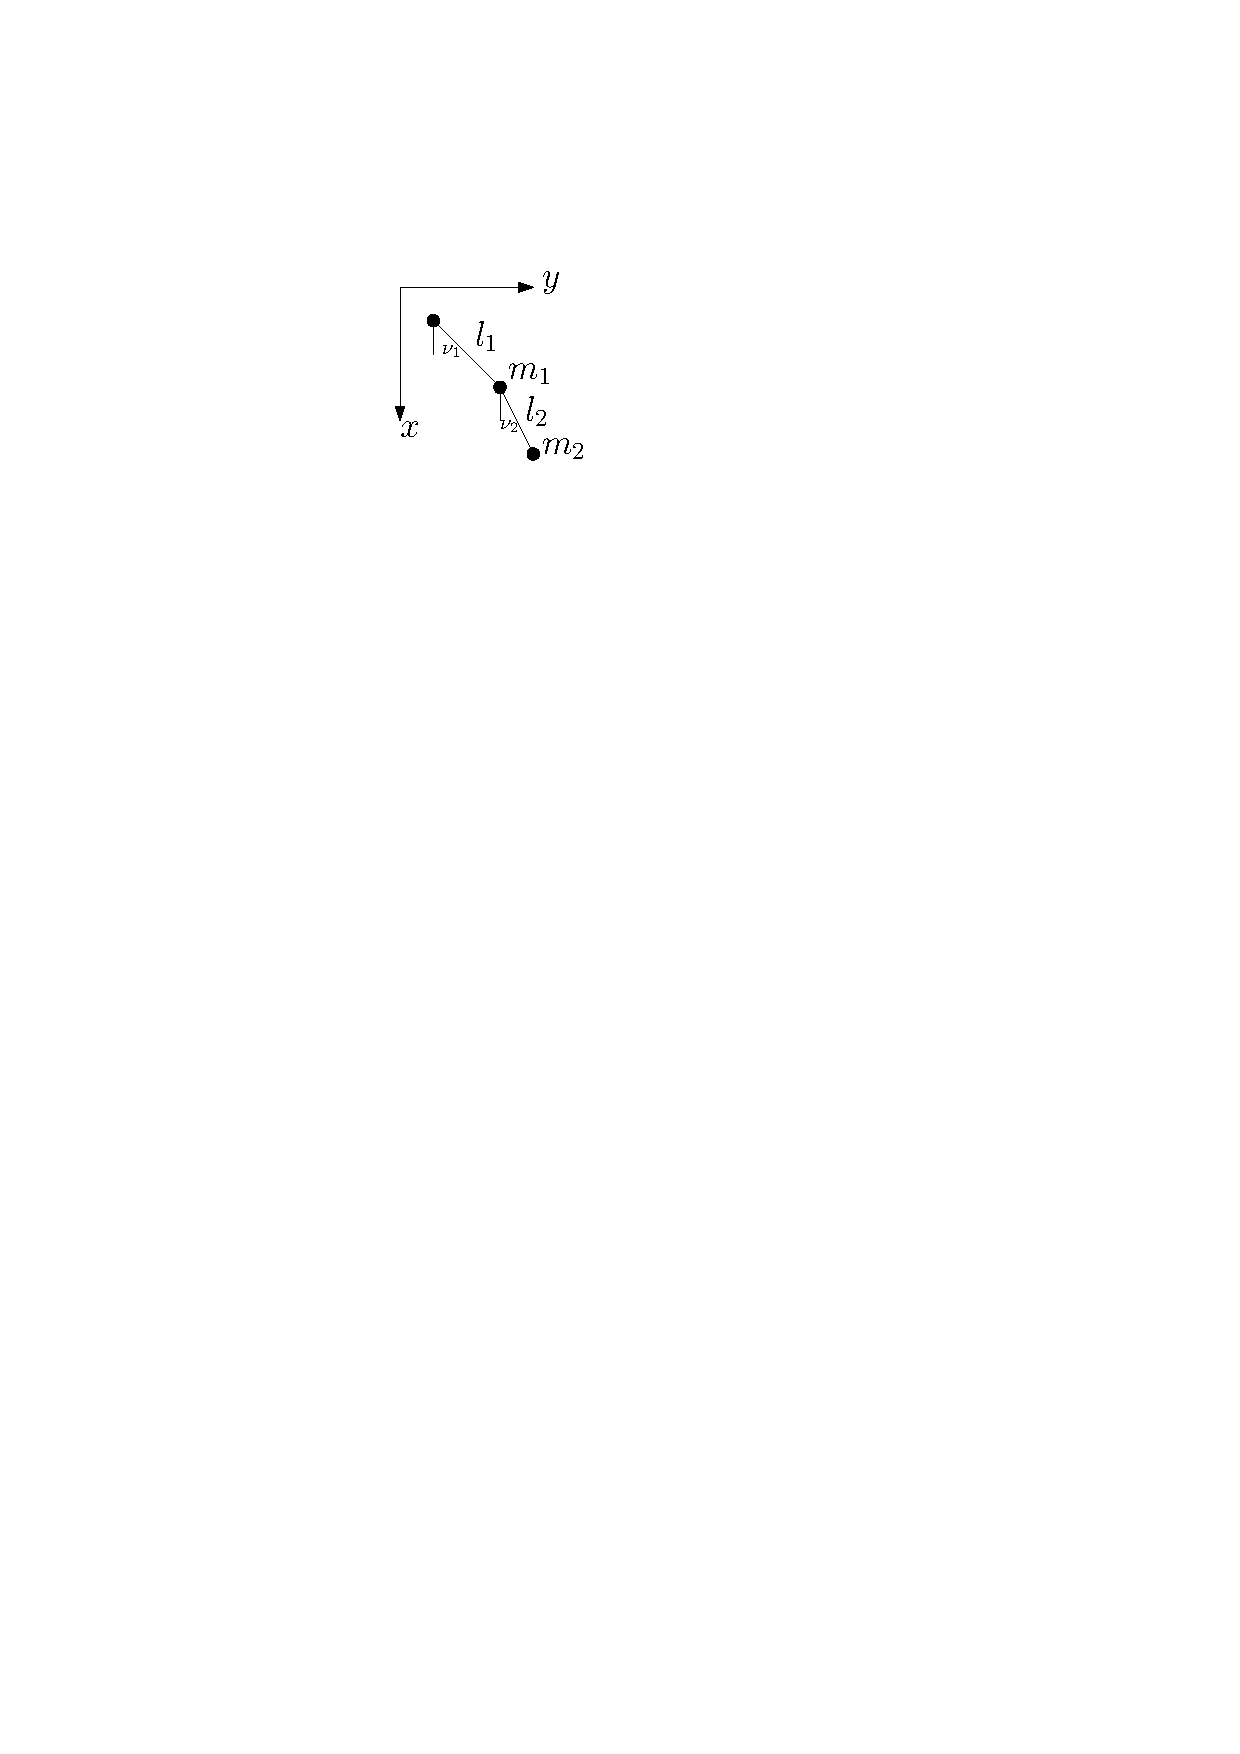
\includegraphics{figures/ch1/doppelpendel}
		\caption{Doppelpendel}
		\label{fig:ch1_doppelpendel}
	\end{figure}
\end{enumerate}


	\chapter{Lagrange-Formalismus}
Aus der Lagrange-Funktion folgt:

\[ \sum_{j=1}^s [ \dfrac{\dint}{\dint t} \dfrac{\partial L}{\partial \dot q_j} - \dfrac{\partial L}{\partial q_i} ] \delta q_i = 0 \]

Damit folgt die Lagrange-Gleichung 2. Art:

\[ \dfrac{\dint}{\dint t} \dfrac{\partial L}{\partial \dot q_j} - \dfrac{\partial L}{\partial q_j} = 0; j = 1, \ldots, s\]


\section{Bemerkungen}
\begin{itemize}
    \item Die Zwangskräfte wurden eliminiert.
    \item Hier sind Energie und Arbeit zentrale Begriffe. Vgl. Kraft und Impuls bei Newton.
    \item Lagrangegleichungen sind invariant unter Punkttransformation.
\end{itemize}


\section{Zyklische Koordinaten}
$q_i$ ist eine {\bf zyklische Koordinate}, gdw. die Lagrange-Funktion nicht explizit von $q_i$ abhängt. Die Lagrange-Funktion kann dabei aber dennoch von $\dot q_i$ abhängen.

\[ q_i \text{ ist zyklische Koordinate} \Leftrightarrow \pdv{L}{q_i} = 0 \Leftrightarrow \pdv{L}{\dot q_i} = \text{const.} \]

\[ \dv{}{t} \pdv{L}{\dot q_i} = 0 \Leftrightarrow \pdv{L}{\dot q_i} = \text{const.} = p_i \]

Dabei ist $\pdv{L}{\dot q_i} = p_i$ der {\bf verallgemeinerte Impuls}.

Zyklische Koordinaten führen immer sofort zu einem {\bf Erhaltungssatz}. Möglichst viele generalisierte Koordinaten sollten zyklisch sein.
	
	\setcounter{chapter}{10}
	\chapter{Übung 1}

\section*{Aufgabe 1}

\begin{description}
	\item[a)] 
	\[
		\frac{(a^2 - b^2)^{-2}}{(a + b)^{-3}} \cdot \frac{(a - b)^2}{a + b}
		= \frac{((a + b)(a - b))^{-2} (a - b)^2}{(a + b)^{-2}}
		= 1
	\] 
	
	\item[b)]
	\[
		\ln(e^{3x} e^{5x}) = \ln(e^{3x + 5x}) 
		= 8x
	\]
	
	\item[c)]
	\[
		\cos(\phi) + \sin(\phi) \tan(\phi) 
		= \frac{\cos^2(\phi)}{\cos(\phi)} \frac{\sin^2(\phi)}{\cos(\phi)}
		= \frac{1}{\cos(\phi)} 
	\]
\end{description}

\section*{Aufgabe 2}

\begin{description}
	\item[a)] 
	\[
		\sdiv{a \cos(x) + \sin(bx + c)}{x} = - a \sin(x) + \cos(bx + c) b
	\] 
	
	\item[b)]
	\[
		\sdiv{(3 + 2x - x^2)e^x}{x} = e^x (3 + 2x - x^2) + (2 - 2x)e^x = e^x (5 - x^2)
	\]
	
	\item[c)]
	\[
		\sdiv{(3 + 4x - x^2)^{1/2}}{x} = (3 + 4x - x^2)^{-1/2} (2 - x)
	\]
	
	\item[d)]
	\[
		\sdiv{x^x}{x} = x^x (\ln(x) + 1)
	\]
\end{description}

\section*{Aufgabe 3}
Die Ableitungen lauten
\begin{align*}
	g'(x) &= 3x^2 - 4x \\	
	g''(x) &= 6x - 4
\end{align*}
und es gilt $g'(x_0) = 0$ genau dann, wenn $x_0 = 0$ oder $x_0 = \frac{4}{3}$. Da $g''(0) = -4 < 0$ liegt dort ein Hochpunkt und da $g''(\frac{4}{3}) = 4 > 0$ liegt dort ein Tiefpunkt.

\section*{Aufgabe 4}
\begin{description}
	\item[a)] 
	\[
		F(x) = \int \frac{x^4 + 2x^2 - 5x + 1}{x} \mathrm{d}x
		= \int x^3 + 2x - 5 + \frac{1}{x} \mathrm{d}x
		= \frac{1}{4} x^4 + x^2 - 5x + \ln(x) + c	
	\]
	\item[b)]
	\begin{description}
		\item[i)] 
		\begin{align*}
			F 
			&= \int^2_1 \mathrm{d} x \ln(x) \int^\infty_{\ln(x)} \mathrm{d} y e^{-y}
			= \int^2_1 \ln(x) \left[ - e^{-y} \right]^\infty_{\ln(x)} \mathrm{d} x \\
			&= \int^2_1 \ln(x) e^{-\ln(x)} \mathrm{d} x
			= \frac{1}{2} \int^2_1 2 \ln(x) \frac{1}{x} \mathrm{d} x
			= \frac{1}{2} \left[ \ln^2(x) \right]^2_1
			= \frac{1}{2} \ln^2(x)
		\end{align*}
		
		\item[ii)] Kopf durch die Wand Methode:
		\[
			F(a) = \int^\infty_{-\infty} x e^{-ax^2} \mathrm{d} x 
			= \left[ -\frac{1}{2a} e^{-ax^2} \right]^\infty_{-\infty}
			= 0
		\]
		
		Kopf Methode: Die Funktion ist Punktsymmetrisch zum Ursprung, also Integral $=0$.
		
		\item[iii)] 
		\begin{align*}
			F(a) &= \int^\infty_{\infty} x^2 e^{-ax^2} \mathrm{d} x 
			= - \int^\infty_{-\infty} \left( \sdiv{}{a} e^{-ax^2} \right) \mathrm{d} x
			= -\sdiv{}{a} \int^\infty_{-\infty} e^{-ax^2} \mathrm{d} x
			= -\sdiv{}{a} \sqrt{\frac{\pi}{a}} \\
			&= \frac{\sqrt{\pi}}{2} a^{-3/2}
		\end{align*}
	\end{description}
\end{description}

\section*{Aufgabe 5}
\begin{description}
	\item[a)]
	\[
		AB - BA
		= \begin{pmatrix}
			1 & 7 \\ 6 & -6
		\end{pmatrix} + 
		\begin{pmatrix}
			6 & -2 \\ 1 & -5
		\end{pmatrix}
		= \begin{pmatrix}
			7 & 5 \\ 7 & -11
		\end{pmatrix}
	\] 
	
	\item[b)]
	\[
		\tr[AB - BA] = -4
	\]
	
	\item[c)]
	\[
		A^{-1} = \frac{1}{\det A} \begin{pmatrix}
			2 & -3 \\
			2 & 1
		\end{pmatrix}
		= \frac{1}{8} \begin{pmatrix}
			2 & -3 \\ 2 & 1
		\end{pmatrix}
	\]
\end{description}
	\chapter{Übung 2}

\section*{Aufgabe 1}

\begin{description}
	\item[a)] $f'(x) = x^3 + 2x - 5 + \frac{1}{x}$
	\item[b)] $f(x) = \cos(x) + \sin(x) \tan(x) = \frac{\cos^2(x)}{\cos(x)} + \frac{\sin^2(x)}{\cos(x)} = \frac{1}{\cos(x)}$, also $f'(x) =\sin(x) \frac{1}{\cos^2(x)} = \frac{\sin(x)}{\cos^2(x)} = \frac{\tan(x)}{\cos(x)}$
	\item[c)] $f(x) = \frac{1}{2 \sqrt{2}} \arctan\left( \frac{2 \sqrt{2}}{1 - x^2} \right)$
	
	Bronstein 6.1.22: $g(x) = \arctan(x)$ $\Rightarrow$ $g'(x) = \frac{1}{1 + x^2}$
	
	Damit: $f'(x) 
	= \frac{1}{2 \sqrt{x}} \frac{1}{1 + \frac{2x^2}{(1 - x^2)^2}} \sqrt{2} \frac{1 - x^2 + 2x^2}{(1 - x^2)^2}
	= \frac{1}{2} \frac{1 + x^2}{(1 - x)^2 + 2x^2}
	= \frac{1}{2} \frac{1 + x^2}{x^4 + 1}$
	
	\item[d)] $f(x) = \frac{1}{4 \sqrt{2}} \log \left( \frac{x^2 + \sqrt{2} x + 1}{x^2 - \sqrt{2}x + 1} \right)$
	
	$f'(x) 
	= \frac{1}{4 \sqrt{2}} \left( \frac{x^2 + \sqrt{2}x + 1}{x^2 - \sqrt{2}x + 1} \right)^{-1} \frac{(2x + \sqrt{2})(x^2 - \sqrt{2}x + 1)-(2x + \sqrt{2})(x^2 + \sqrt{2}x + 1)}{(x^2 + \sqrt{2}x + 1)^2}
	= \dots 
	= \frac{1}{2} \frac{1 - x^2}{x^4 + 1}$
\end{description}

\section*{Aufgabe 2}

\begin{description}
	\item[a)] $f(x) = \cos(x)$, $f'(x) = -\sin(x)$, $f''(x) = -\cos(x)$, also $f(0) = 1$, $f'(0) = 0$, $f''(0) = -1$.
	
	Damit ergibt sich: $f(x) = 1 + 0 x + \left( -\frac{1}{2} \right)x^2 + \mathcal{O}(x^3) \approx 1 - \frac{x^2}{2}$
	
	\item[b)] $f(x) = \log(1 - x)$, $f'(x) = -\frac{1}{1 - x} = \frac{1}{x - 1}$, $f''(x) = -\frac{1}{(x - 1)^2}$, also $f(0) = 0$, $f'(0) = 1$, $f''(0) = -1$.
	
	Damit ergibt sich: $f(x) = -x - \frac{x^2}{2} + \mathcal{O}(x^3)$.
\end{description}

\section*{Aufgabe 3}

\begin{description}
	\item[a)] $f(x) = e^{\lambda x} \sin(3x)$, man rechne:
	\begin{align*}
		\int e^{\lambda x} \sin(3x) \mathrm{d} x	
		&= \frac{1}{\lambda} e^{\lambda x} \sin(3x) - \frac{3}{\lambda} \int e^{\lambda x} \cos(3x) \mathrm{d} x \\
		&= \frac{1}{\lambda} e^{\lambda x} \sin(3x) - \frac{3}{\lambda} \left[ \frac{1}{\lambda} e^{\lambda x} \cos(3x) + \frac{3}{\lambda} \int e^{\lambda x} \sin(3x) \mathrm{d} x \right]
	\end{align*}
	
	Damit ergibt sich:
	\[
		\left( 1 + \frac{9}{\lambda^2} \right) \int e^{\lambda x} \sin(3x) \mathrm{d} x = \frac{1}{\lambda^2} e^{\lambda x} \left( \lambda \sin(3x) - 3 \cos(3x) \right)	
	\]
	
	Noch durch den Vorfaktor teilen:
	\[
		\int e^{\lambda x} \sin(3x) \mathrm{d} x 
		= \frac{1}{\lambda^2 + 9} e^{\lambda x} \left( \lambda \sin(3x) - 3 \cos(3x) \right) + C
	\]

	\item[b)] Stichwort: Partialbruchzerlegung
	\[ 
		\frac{1}{(1 - x)(1 + x)} 
		= \frac{A}{1 - x} + \frac{B}{1 + x} 
		= \frac{A + Ax + B - Bx}{(1 - x)(1 + x)} 
		= \frac{x(A - B) + (A + B)}{(x - 1)(x + 1)}
	\]
	Vergleich: $A = \frac{1}{2}$, $B = \frac{1}{2}$
	
	Nun einfach:
	\begin{align*}
		\int \frac{1}{(x - 1)(x + 1)} \mathrm{d} x 
		&= \int \frac{1}{2} \frac{1}{x - 1} + \frac{1}{2} \frac{1}{1 + x} \mathrm{d} x 
		= - \frac{1}{2} \log(1 - x) + \frac{1}{2} \log(1 + x) + C \\
		&= \frac{1}{2} \log \left( \frac{1 + x}{1 - x} \right) + C
	\end{align*}

	\item[b, i)] Verwende Substitution $x = \sin(z)$, $\frac{\mathrm{d} x}{\mathrm{d} z} = \cos(z)$, $z = \arcsin(x)$
	
	\begin{align*}
		\int_0^1 \frac{\mathrm{d} x}{\sqrt{1 - x^2}}	 
		&= \int^{\pi/2}_{0} \frac{1}{\sqrt{1 - \sin^2(z)}} \frac{\mathrm{d} x}{\mathrm{d} z} \mathrm{d} z
		= \int^{\pi / 2}_0 \frac{1}{\cos(z)} \cos(z) \mathrm{d} z
		= \int^{\pi / 2}_0 1 \mathrm{d} z \\
		&= \left[ z \right]^{\pi / 2}_0 = \frac{\pi}{2}
	\end{align*}

	\item[b, ii)]  $F(a, n) = \int^\infty_{-\infty} x^{2n} e^{-ax^2} \mathrm{d} x$ mit $a > 0$
	\begin{align*}
			F(a, n) 
			&= \left( \frac{\mathrm{d}}{\mathrm{d} a} \right)^n (-1)^n \int^{\infty}_{-\infty} e^{-ax^2} \mathrm{d} x
			= \left( \frac{\mathrm{d}}{\mathrm{d} a} \right)^n (-1)^n \sqrt{\frac{\pi}{a}} \\
			&=  \sqrt{\pi} \frac{\mathrm{d}^n}{\mathrm{d} a^n} \left( a^{-1/2} \right) (-1)^n
			= \sqrt{\pi} (-1)^n \frac{\mathrm{d}^{n -1}}{\mathrm{d} a^{n - 1}} \left( -\frac{1}{2} a^{-3/2} \right) \\
			&= \sqrt{\pi} (-1)^n \frac{\mathrm{d}^{n - 2}}{\mathrm{d} a^{n - 2}} \left( \frac{1}{2} \frac{3}{2} a^{-5/2} \right) 
			= \dots 
			= \sqrt{\pi} (-1)^n (-1)^n \left( \frac{1}{2} \frac{3}{2} \cdot \hdots \cdot \frac{2n - 1}{2} a^{-(2n + 1)/2} \right) \\
			&= \dots
	\end{align*}
\end{description}

\section*{Aufgabe 4}

\begin{description}
	\item[a)] 
	\begin{tabular}{|c||c|c|c|c|c|c|c|c|}
		\hline 
		$z = x + iy$ & $1 + 1i$ & $3 - 4i$ & $-3 + 2i$ & -2 & $5 - 12 i$ & $-1 - i$ & 1 + 1.7i \\
		\hline
		$r = \mabs{z}$ & $\sqrt{2}$ & $5$ & $\sqrt{13}$ & $2$ & $13$ & $\sqrt{2}$ & 2 \\
		\hline 
		$\phi = \arg(z)$ & $\frac{\pi}{4}$ & $1.705 \pi$ & $0.813 \pi$ & $\pi$ & $1.626 \pi$ & $\frac{5}{4} \pi$ & $-\pi/3$ \\
		\hline 
	\end{tabular}
 
	\item[b, i)] $z = \frac{1 + i}{2 + 3i} = \frac{(1 + i)(2 - 3i)}{(2 + 3i)(2 - 3i)} = \dots = \frac{5 - i}{13} \approx \frac{1}{13} \sqrt{26} e^{1.937 \pi i}$
	
	\item[b, ii)] $z = \frac{1}{\sqrt{1 + i}} = (1 + i)^{-1/2} = \left( \sqrt{2}\exp^{i \frac{\pi}{4}} \right)^{-1/2}$
	
		$z'_1 = 2^{-1/4} e^{-i \frac{\pi}{8} + 2 \pi i}$
		
		$z'_2 = 2^{-1/4} e^{-i \frac{9}{8} \pi + 2 \pi i}$
\end{description}
	\chapter*{Übung 3}

\section*{Aufgabe 5}

\begin{description}
	\item[a)] $\vec{r}(t) = (a \cos(\omega t), b \sin(\omega t))$, oder getrennt: $x(t) = a \cos(\omega t)$ und $y(t) = b \sin(\omega t)$.

Beobachte: $\left( \frac{x(t)}{a} \right)^2 + \left( \frac{y(t)}{b} \right)^2 = \sin^2(\omega t) + \cos^2(\omega t) = 1$. Das ist eine Ellipse (siehe Abbildung \ref{fig:ueb3_aufgabe5a}).

	\begin{figure}[h]
		\centering
		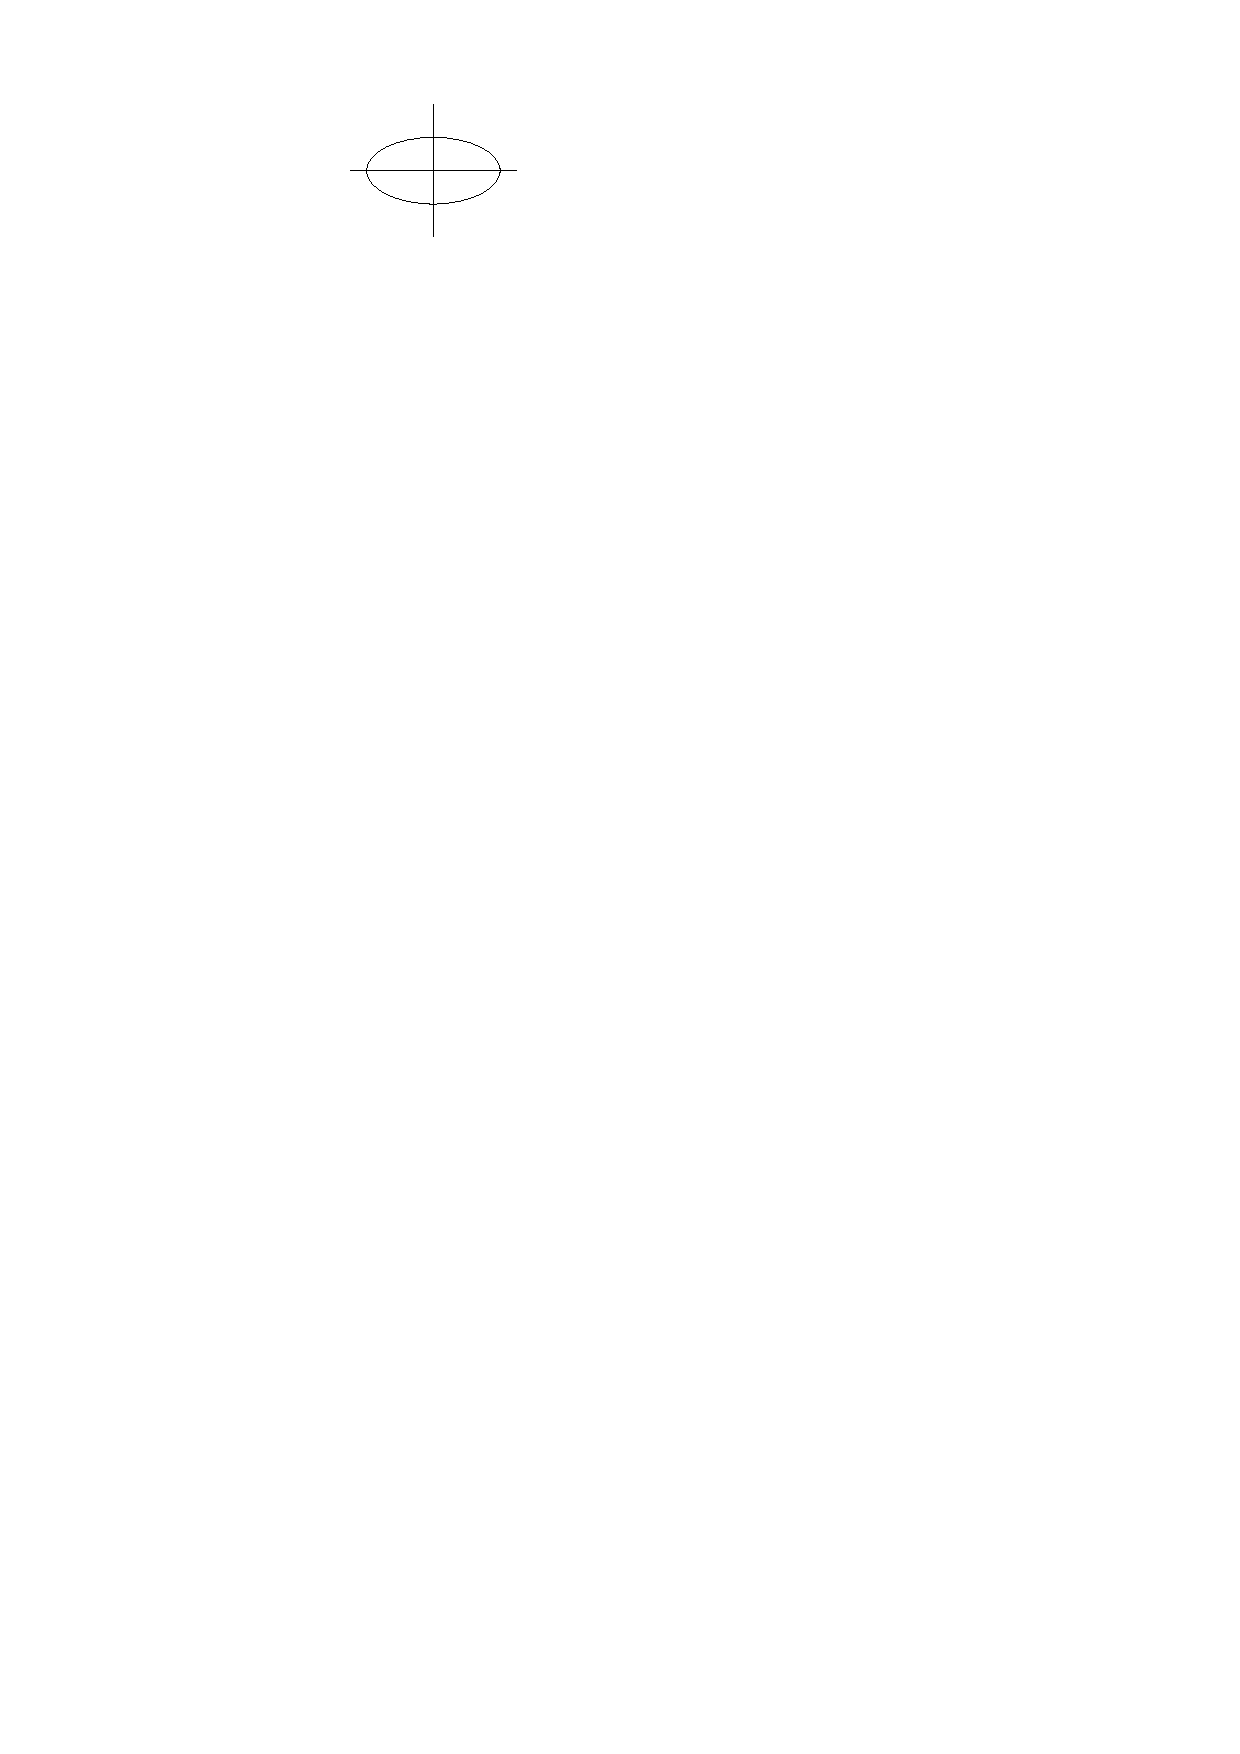
\includegraphics{figures/ueb3/aufgabe5a}
		\caption{Eine Ellipse.}
		\label{fig:ueb3_aufgabe5a}
	\end{figure}

	\item[b, i)] $\vec{r}(t) = (a \cos(\omega t), a \sin(\omega t), c t)$, oder getrennt: $x(t) = a \cos(\omega t)$, $y(t) = a \sin(\omega t)$ und $z(t) = ct$.
	 
	Das ist ein Kreis mit einem linearen "`displacement"' in der $z$-Achse; also eine Art Schraube.
	
	\item[b, ii)] Wir suchen $\Delta z = z(t_2) - z(t_1)$, wobei $x(t_1) = x(t_2)$ und $y(t_1) - y(t_2)$. Man nennt $\Delta z$ auch "`helicoid step"'.
	
	Einsetzen: $x(t_1) = \cos(\omega t_1)$, $x(t_2) = \cos(\omega t_2)$; also $x(t_1) = x(t_2)$ genau dann, wenn $\omega t_1 = \omega t_2 + 2 \pi n$ mit $n \in \mathbb{N}$. Also erfüllt für $\Delta t = \frac{2 \pi}{\omega}$ und Vielfache davon. Damit: $\Delta z = c (t_2 - t_1) = c \Delta t = \frac{2 \pi c}{\omega}$. $\frac{2 \pi}{\omega} =: T$ ist die Periode.
	
	\item[c)] Rechne 
	\begin{align*}
		\vec{v}(t) &= \msimplediff{\vec{r}}{t} = (-r \omega \sin(\omega t), r \omega \cos(\omega t), 0) \\
		\vec{a}(t) &= \msimplediff{\vec{v}}{t} = (-r \omega^2 \cos(\omega t), -r \omega^2 \sin(\omega t), 0) = -\omega^2 \vec{r}(t)
		\text{.}
	\end{align*}
	Siehe Abbildung \ref{fig:ueb3_aufgabe5c} für die Visualisierung der drei Vektoren.
	
	\begin{figure}[h]
		\centering
		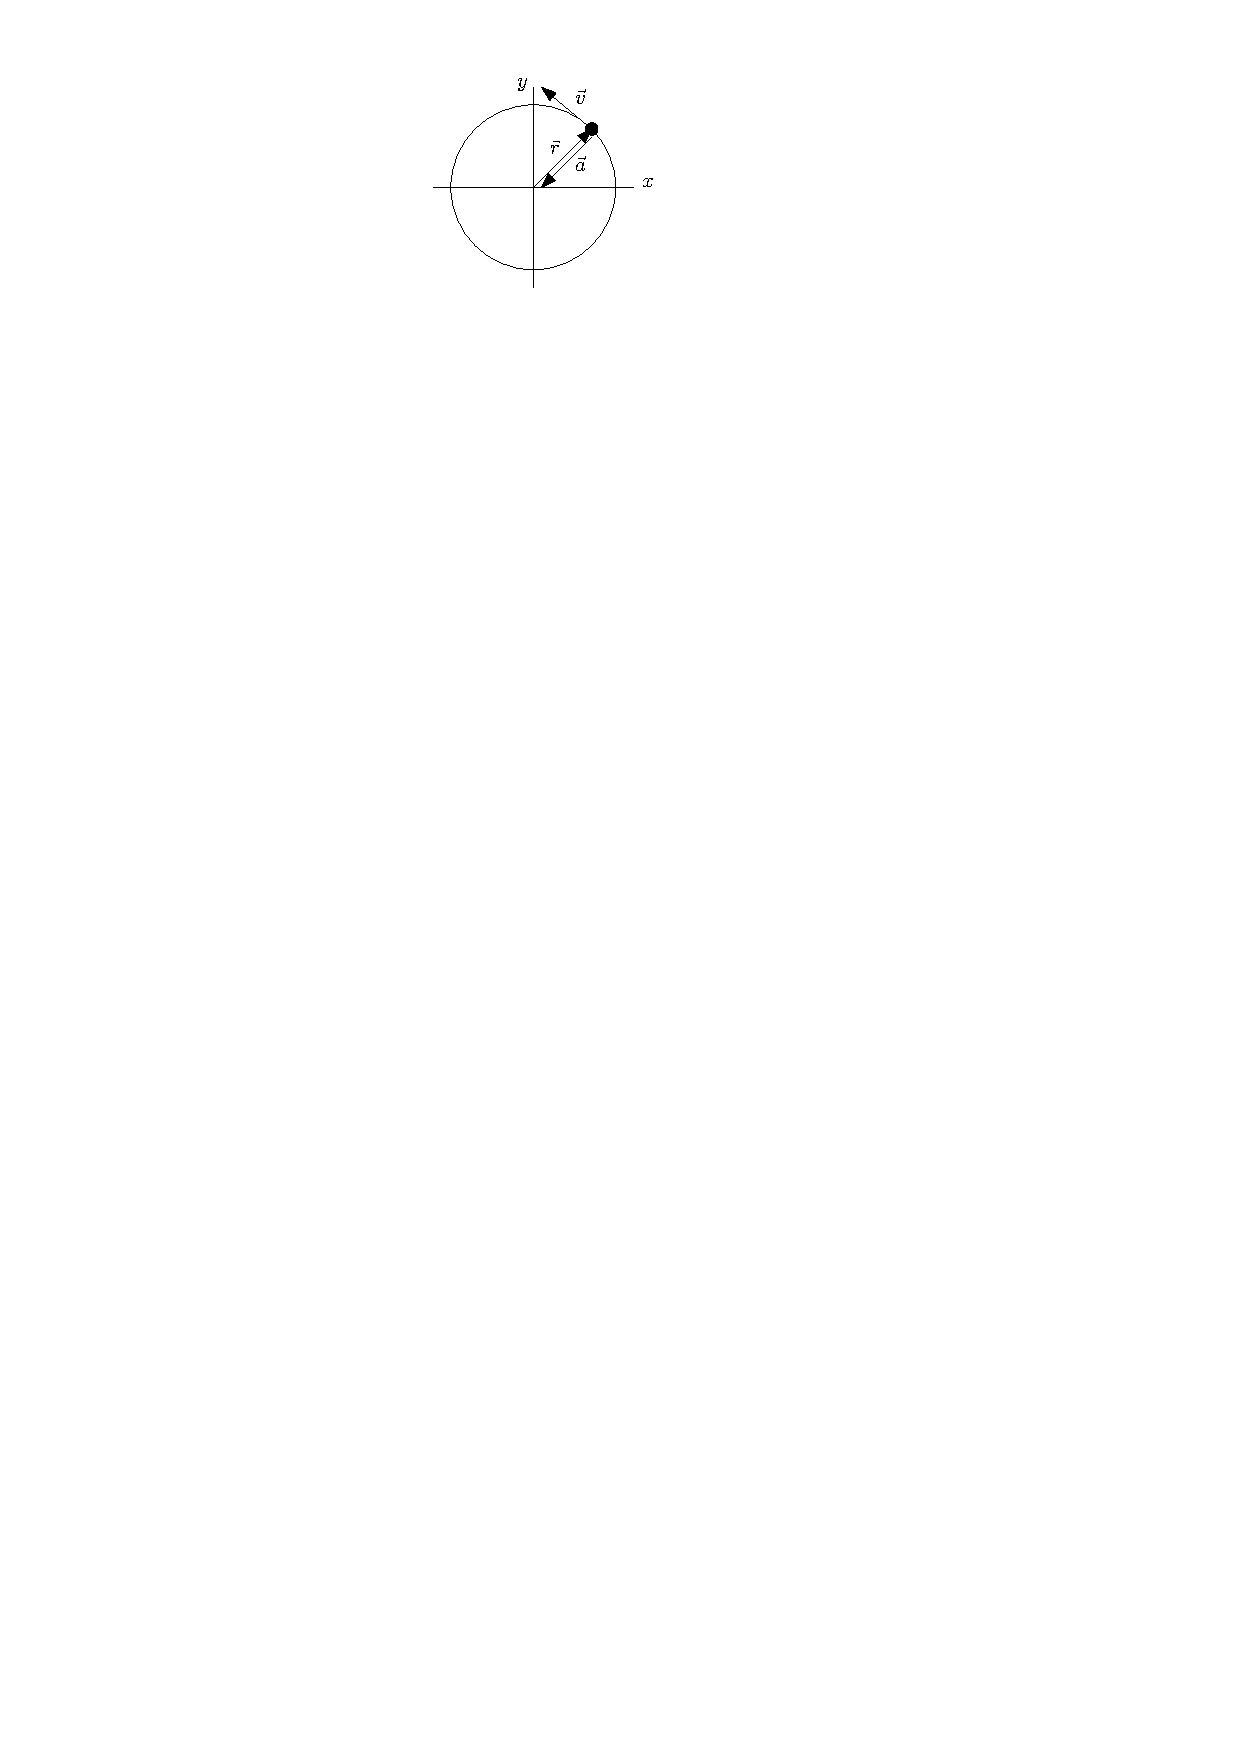
\includegraphics{figures/ueb3/aufgabe5c}
		\caption{Vektore $\vec{r}$, $\vec{v}$ und $\vec{a}$ bei Aufgabe 5c.}
		\label{fig:ueb3_aufgabe5c}
	\end{figure}
	
	Für die Kreisbahn muss nun gelten: $-G \frac{M_e m_s}{r^3} \vec{r} \overset{!}{=} -m_s \omega^2 \vec{r}$. Dass das $m_s$ auf beiden Seiten gleich ist, ist alles andere als trivial und führt auf Einstein zurück; aktuell ist uns das aber egal.
	
	Mit Kürzen erhalten wir
	\[
		-G \frac{M_e}{r^3} \overset{!}{=} -\omega^2 \quad \Rightarrow \quad \omega = \sqrt{ \frac{G M_e}{r} } \frac{1}{r}
		\text{.}
	\]
	
	Beobachtung: $T^2 \approx r^3$; das ist Kepler's Dritte Gesetz.
\end{description}

\section*{Aufgabe 6}

Siehe Abbildung \ref{fig:ueb3_aufgabe6} für eine Skizze. Es gilt $\vec{a} = \msimplediff{\vec{v}}{t}$, also $\mathrm{d} \vec{v} = \vec{a} \mathrm{d} t$. Das integrieren wir:
	\begin{align*}
		& \int_{\vec{v}_0}^{\vec{v}} \mathrm{d} \vec{v}' = \int_{t = 0}^{t} \vec{a} \mathrm{d} t' \\
		\Rightarrow &~ \vec{v} - \vec{v}_0 = (0, 0, -gt) \\
		\Rightarrow &~ \vec{v} = \vec{v}_0 + (0, 0, -gt) = (v \cos(\alpha), 0, v \sin(\alpha) - gt)
		\text{.}
	\end{align*}
	
	Das gleiche Spiel nochmal:
	\[
		\vec{r} = \msimplediff{\vec{v}}{t} 
		\quad \Rightarrow \quad \int_{\vec{r_0}}^{\vec{r}} \mathrm{d} \vec{r}' = \int_{t = 0}^t \vec{v} \mathrm{d} t'
		\quad \Rightarrow \quad \vec{r}(t) - \vec{r}_0 = (v \cos(\alpha t), 0, v \sin(\alpha t) - \frac{1}{2} g t^2)
	\]
	
	Oder getrennt geschrieben: $x(t) = v \cos(\alpha t)$, $y(t) = 0$ und $z(t) = v \sin(\alpha t) - \frac{1}{2} g t^2$. Beobachtung: $z(t)$ wird an zwei Punkten $0$: für $t = 0$ und für $t = \frac{2 v \sin(\alpha)}{g}$.
	
	\begin{figure}[h]
		\centering
		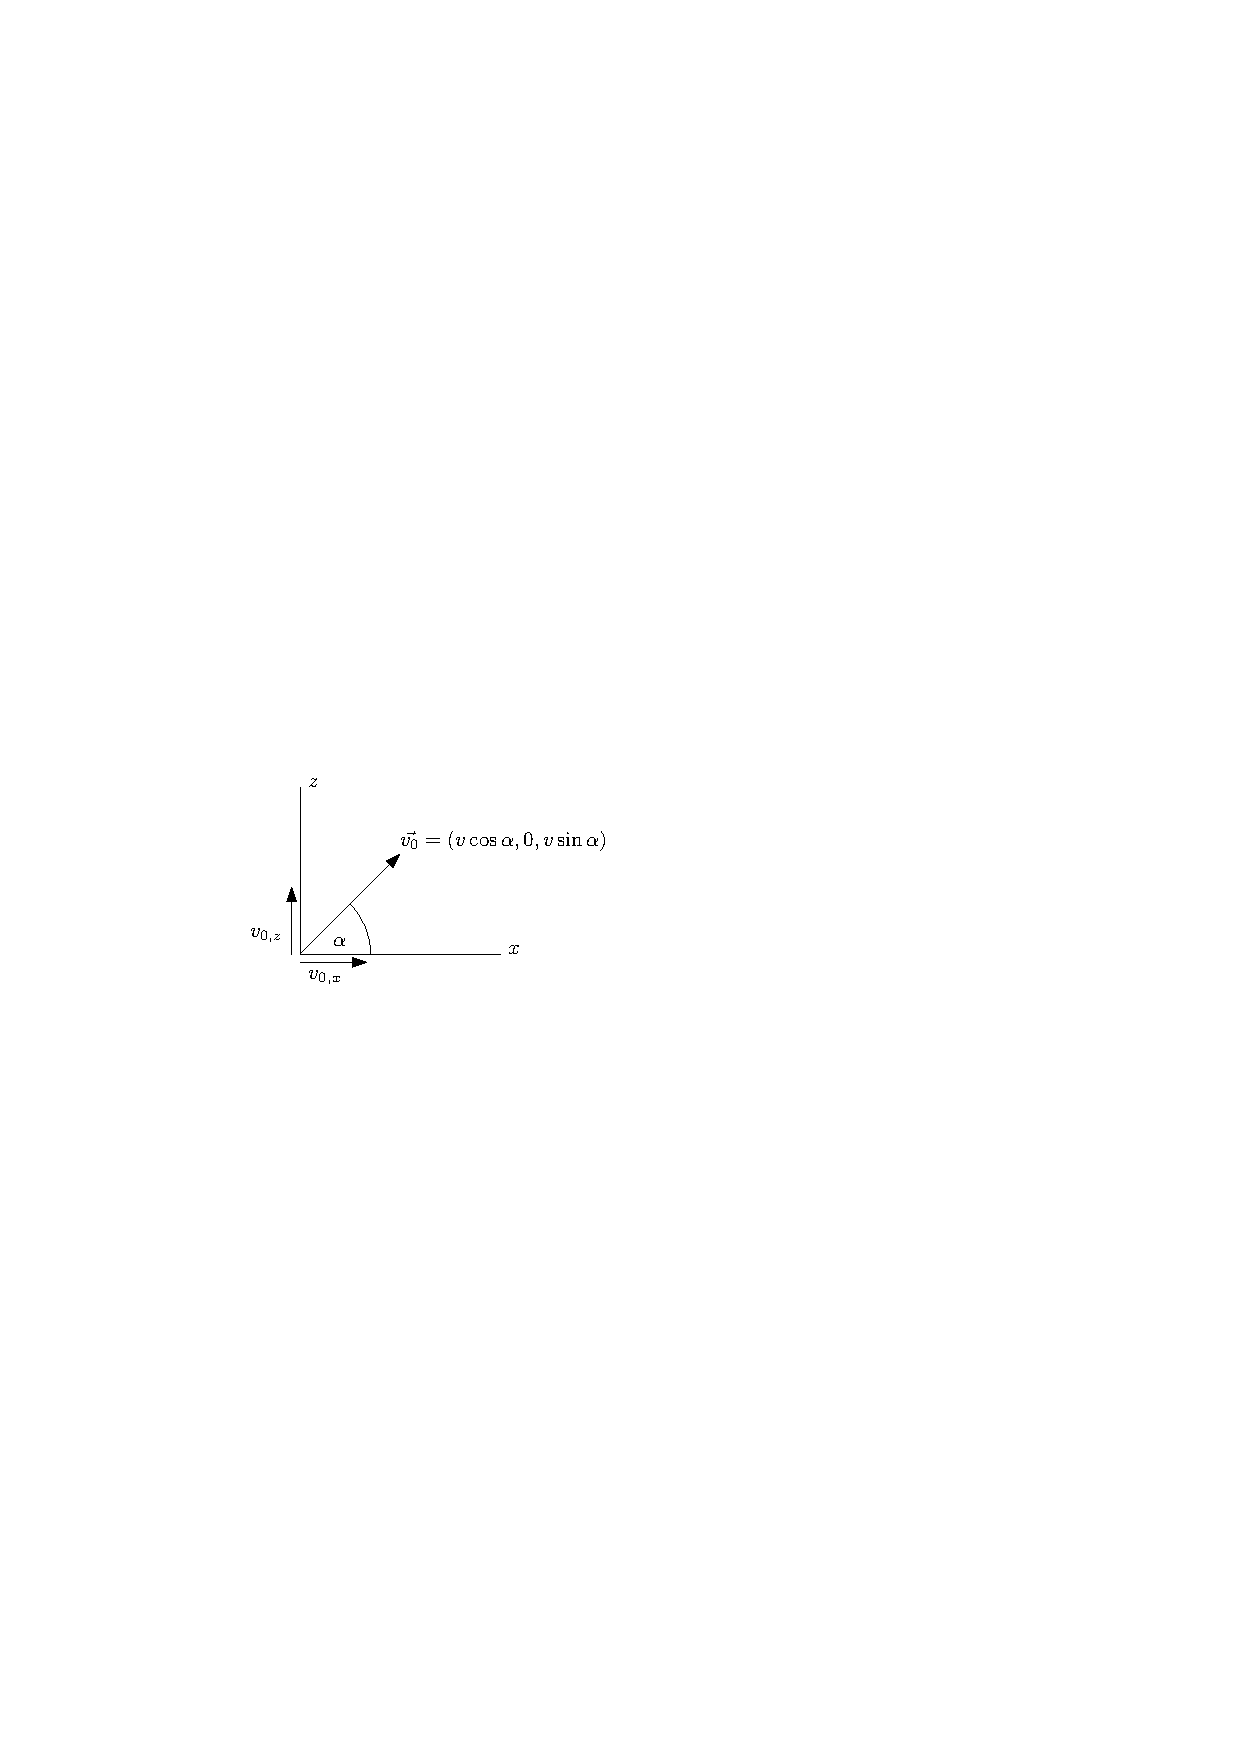
\includegraphics{figures/ueb3/aufgabe6}
		\caption{Eingangssituation in Aufgabe 6.}
		\label{fig:ueb3_aufgabe6}
	\end{figure}
	
	Aus der $x$-Gleichungen erhalten wir $t = \frac{x}{v \cos(\alpha)}$. Also $z(x) = x \tan(\alpha) - \frac{gx^2}{2 v^2 \cos^2(\alpha)}$. Das ist eine Parabel. Die Nullstellen von $z(x)$ sind $x = 0$ und $x = \frac{2 v^2 \sin(\alpha) \cos(\alpha)}{g} = v \cos(\alpha) \underbrace{\frac{2 v \sin(\alpha)}{g}}_{\text{Nullstelle von $z(t)$}}$.
	
	Für welches $\alpha'$ wird ist die Wurfweite maximal? Maximiere $x_{\text{reach}}(\alpha)$. Es gilt
	\[
		\msimplediff{x_{\text{reach}}(\alpha)}{\alpha} = \frac{2v^2}{g} (\cos^2(\alpha) \sin^2(\alpha)) = \frac{2 v^2}{g} \cos(2 \alpha)
		\text{.}
	\]
	Eine Nullstelle $\alpha'$ davon erfüllt $\cos(2 \alpha') = 0$, also $2 \alpha' = \frac{\pi}{2}$ und damit $\alpha' = \frac{\pi}{4}$.

\section*{Aufgabe 7}

Für eine Skizze siehe Abbildung \ref{fig:ueb3_aufgabe7}.

\begin{figure}[h]
	\centering
	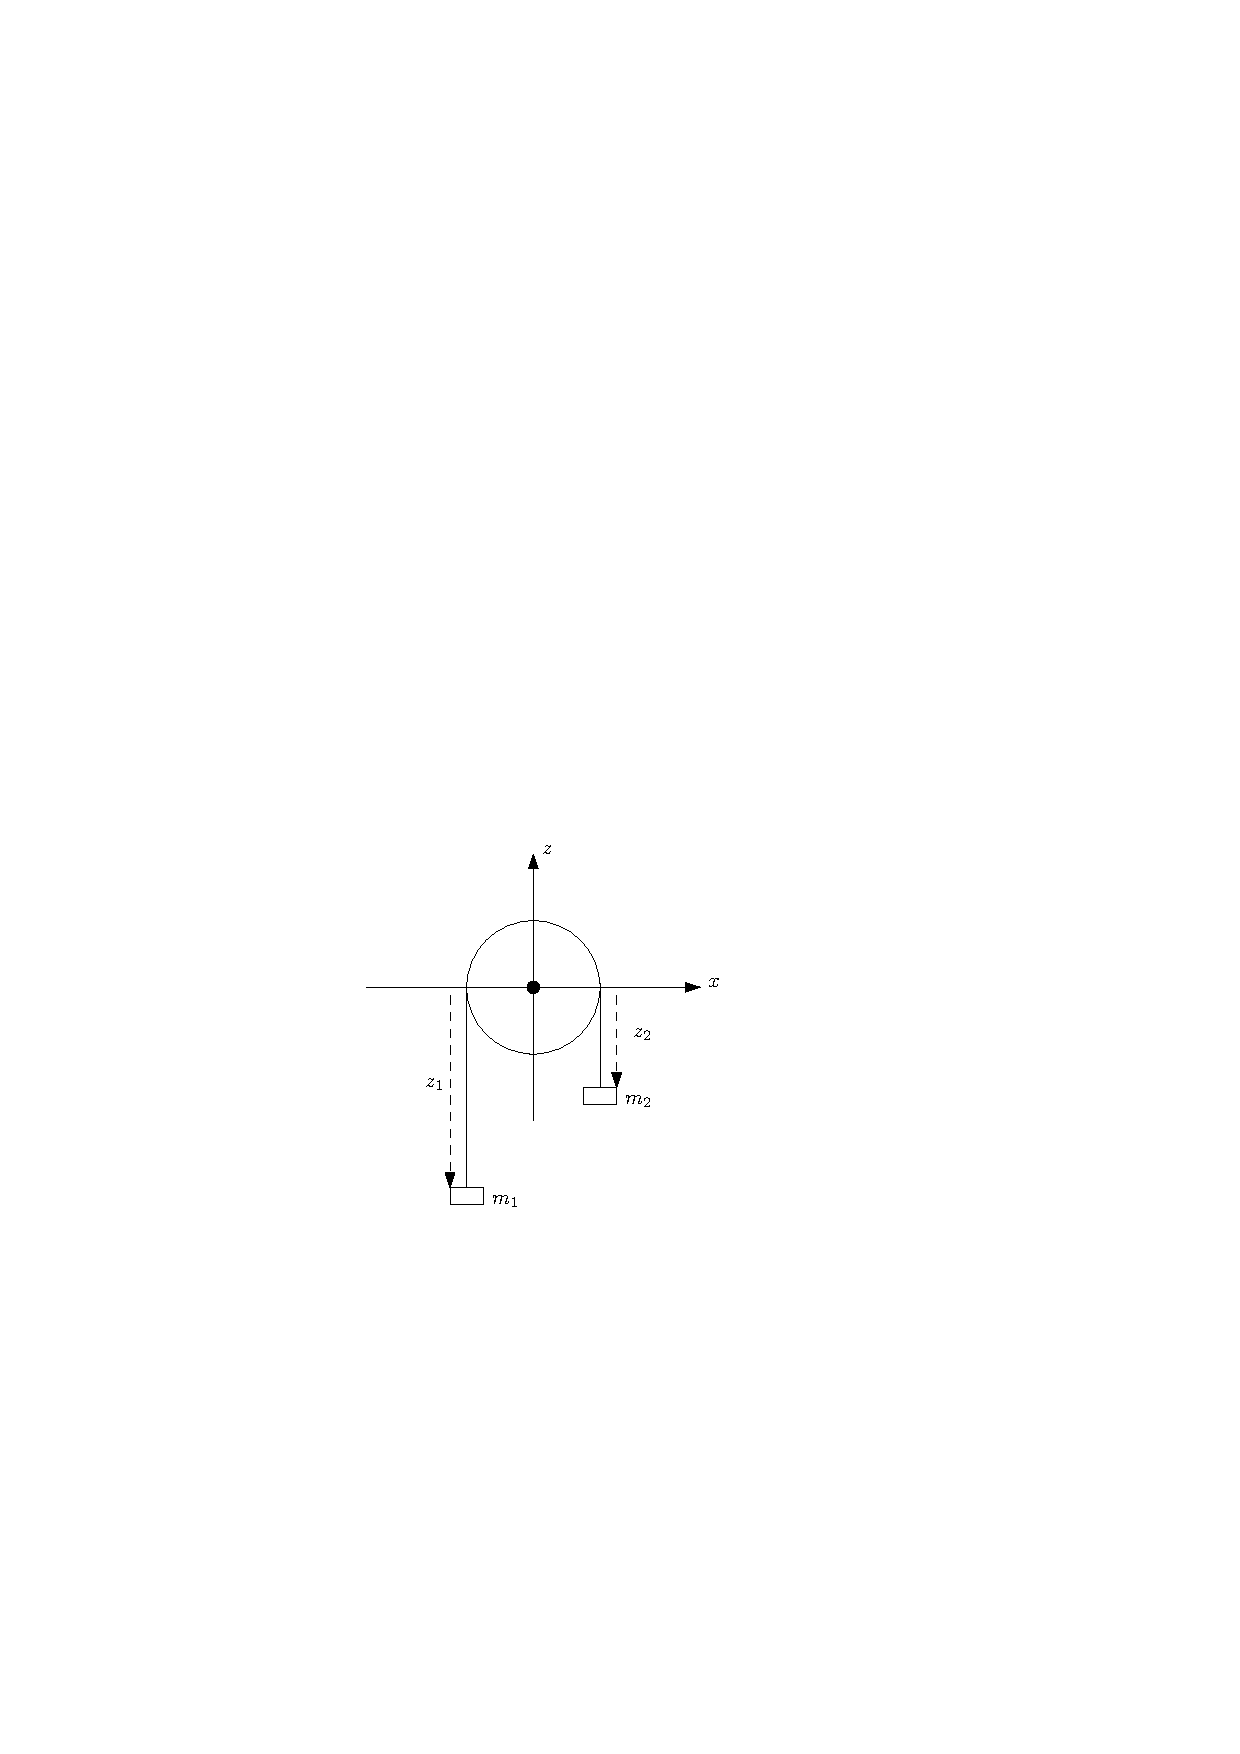
\includegraphics{figures/ueb3/aufgabe7}
	\caption{Die Massen $m_1$ und $m_2$ können sich nur vertikal bewegen.}
	\label{fig:ueb3_aufgabe7}
\end{figure}

Die generalisierten Koordinaten(?,\footnote{nur $(z_1, \dot(z)_1)$ sind generalisierte Koordinaten?}) sind $(z_1, z_2, \dot{z}_1, \dot{z}_2)$ und die Constraints sind Maximale Länge des Fadens, $l = \mabs{z_1} + \mabs{z_2} = -z_1 - z_2$.

Nun die Lagrange-Funktion aufstellen (beachte: $g < 0$, $z_2 = -z_1 - l$, $\dot{z}_2 = \dot{z}_1$): 
\begin{align*}
	L(z_1, z_2, \dot{z}_1, \dot{z}_2) 
	&= T - V = \sum_i T_i - V_i \\
	&= \frac{1}{2} m_1 \vec{z}_1^2 + \frac{1}{2} m_2 \dot{z}_2^2 + m_1 z_1 g + m_2 z_2 g \\
	&= \frac{1}{2} (m_1 + m_2) \dot{z}_1^2 + (m_1 - m_2) g z_1 - m_2 g l
	\text{.}
\end{align*}
Durch das Constraint konnten wir die Lagrange-Funktion also mit nur $(z_1, \dot{z}_1)$ statt $(z_1, z_2, \dot{z}_1, \dot{z}_2)$ ausdrücken.

Anders ausgedrückt: 2 Teilchen, die sich in 1D bewegen, haben zwei Grad Freiheit; das führt auf $4$ Koordinaten. Da wir aber ein Constraint haben, gibt es nur noch ein Grad Freiheit, für das wir nur noch ein Paar Koordinaten brauchen.

Nun muss gelten $\msimplediff{}{t} \frac{\partial L}{\partial \dot{z}_1} = \frac{\partial L}{\partial z_1}$, wobei
\begin{align*}
	\frac{\partial L}{\partial z_1} &= (m_1 - m_2) g, \\
	\msimplediff{}{t} \frac{\partial L}{\partial \dot{z}_1} &= (m_1 + m_2) \ddot{z}_1 
	\text{.}
\end{align*}
Also $(m_1 + m_2) \ddot{z}_1 = (m_1 - m_2) g$ und damit \fbox{$\ddot{z}_1 = g \frac{m_1 - m_2}{m_1 + m_2}$}.


	\chapter*{Übung 4}

\section*{Aufgabe 8}

Erinnerung: $\dot{x}(t) = \msimplediff{x(t)}{t}$ und $\ddot{x}(t) = \frac{\mathrm{d}^2 x(t)}{\mathrm{d} t^2}$.

Zu lösende Gleichung:
\[
	\ddot{x}(t) = -\frac{k}{m} x(t)
	\text{.}
\]

Ansatz: $x(t) = c_\lambda e^{\lambda t}$; also $\dot{x}(t) = \lambda c_\lambda e^{\lambda t}$ und $\ddot{x}(t) = \lambda^2 c_\lambda e^{\lambda t}$. Das in die zu lösende Gleichung einsetzen:
\[
	\lambda^2 c_\lambda c^{\lambda t} = -\frac{k}{m} c_\lambda e^{\lambda t}
	\quad \Longleftrightarrow \quad
	\lambda^2 = -\frac{k}{m}
	\quad \Longrightarrow \quad
	\lambda = \pm i \sqrt{\frac{k}{m}}
	\text{.}
\]

Die allgemeine Lösung lautet also: $x(t) = c_1 e^{it \sqrt{k / m}} + c_2 e^{-it \sqrt{k / m}}$ und die Ableitung davn ist: $\dot{x}(t) = \sqrt{\frac{k}{m}} \left( c_1 e^{it \sqrt{k / m}} - c_2 e^{-it \sqrt{k / m}} \right)$.

Nun sollen die Konstanten $c_1$ und $c_2$ bestimmt werden. Dazu die Anfangsbedingungen einsetzen:
\begin{align*}
	x_0 &\overset{!}{=} x(t = 0) = c_1 + c_2,	 \\
	v_0 &\overset{!}{=} \dot{x}(t = 0) = i \sqrt{\frac{k}{m}} (c_1 - c_2)
	\text{.}
\end{align*}
Das führt auf $c_1 = \frac{1}{2} \left( x_0 + \frac{1}{i} \sqrt{\frac{m}{k}} v_0 \right)$ und $c_2 = \frac{1}{2} \left( x_0 - \frac{1}{i} \sqrt{\frac{m}{k}} v_0 \right)$. Eingesetzt ergibt das die Lösung
\[
	x(t) = \frac{1}{2} x_0 \left( e^{it \sqrt{k / m}} + e^{-it \sqrt{k / m}} \right)
	+ \frac{1}{2i} \sqrt{\frac{m}{k}} v_0 \left( e^{it \sqrt{k / m}} - e^{-it \sqrt{k / m}} \right)
	\text{.}
\]

Um den Term weiter zu vereinfachen, verwende $\frac{k}{m} = \omega^2$. Das führt auf auf die vereinfachte Lösung
\[
	x(t) = x_0 \cos(\omega t) + \frac{v_0}{\omega} \sin(\omega t)
	\text{.}
\]

Zuletzt berechnen wir die Energie, wobei $\dot{x}(t) = -x_0 \omega \sin(\omega t) + v_0 \omega \cos(\omega t)$:
\begin{align*}
	E &= T + V = \frac{1}{2} m \dot{x}^2 + \frac{1}{2} k x^2	 = \frac{1}{2} m \left( \dot{x}^2(t) + \omega^2 x^2(t) \right) \\
	&= \dots = \frac{1}{2} m \left( v_0^2 + \omega^2 x_0^2 \right) = \frac{1}{2} m v_0^2 + \frac{1}{2} k x_0^2
	\text{.}
\end{align*}

\section*{Aufgabe 9}
Siehe Abbildung \ref{fig:ueb4_aufgabe9} für eine Skizze mit den Variablen.

\begin{figure}[h]
	\centering
	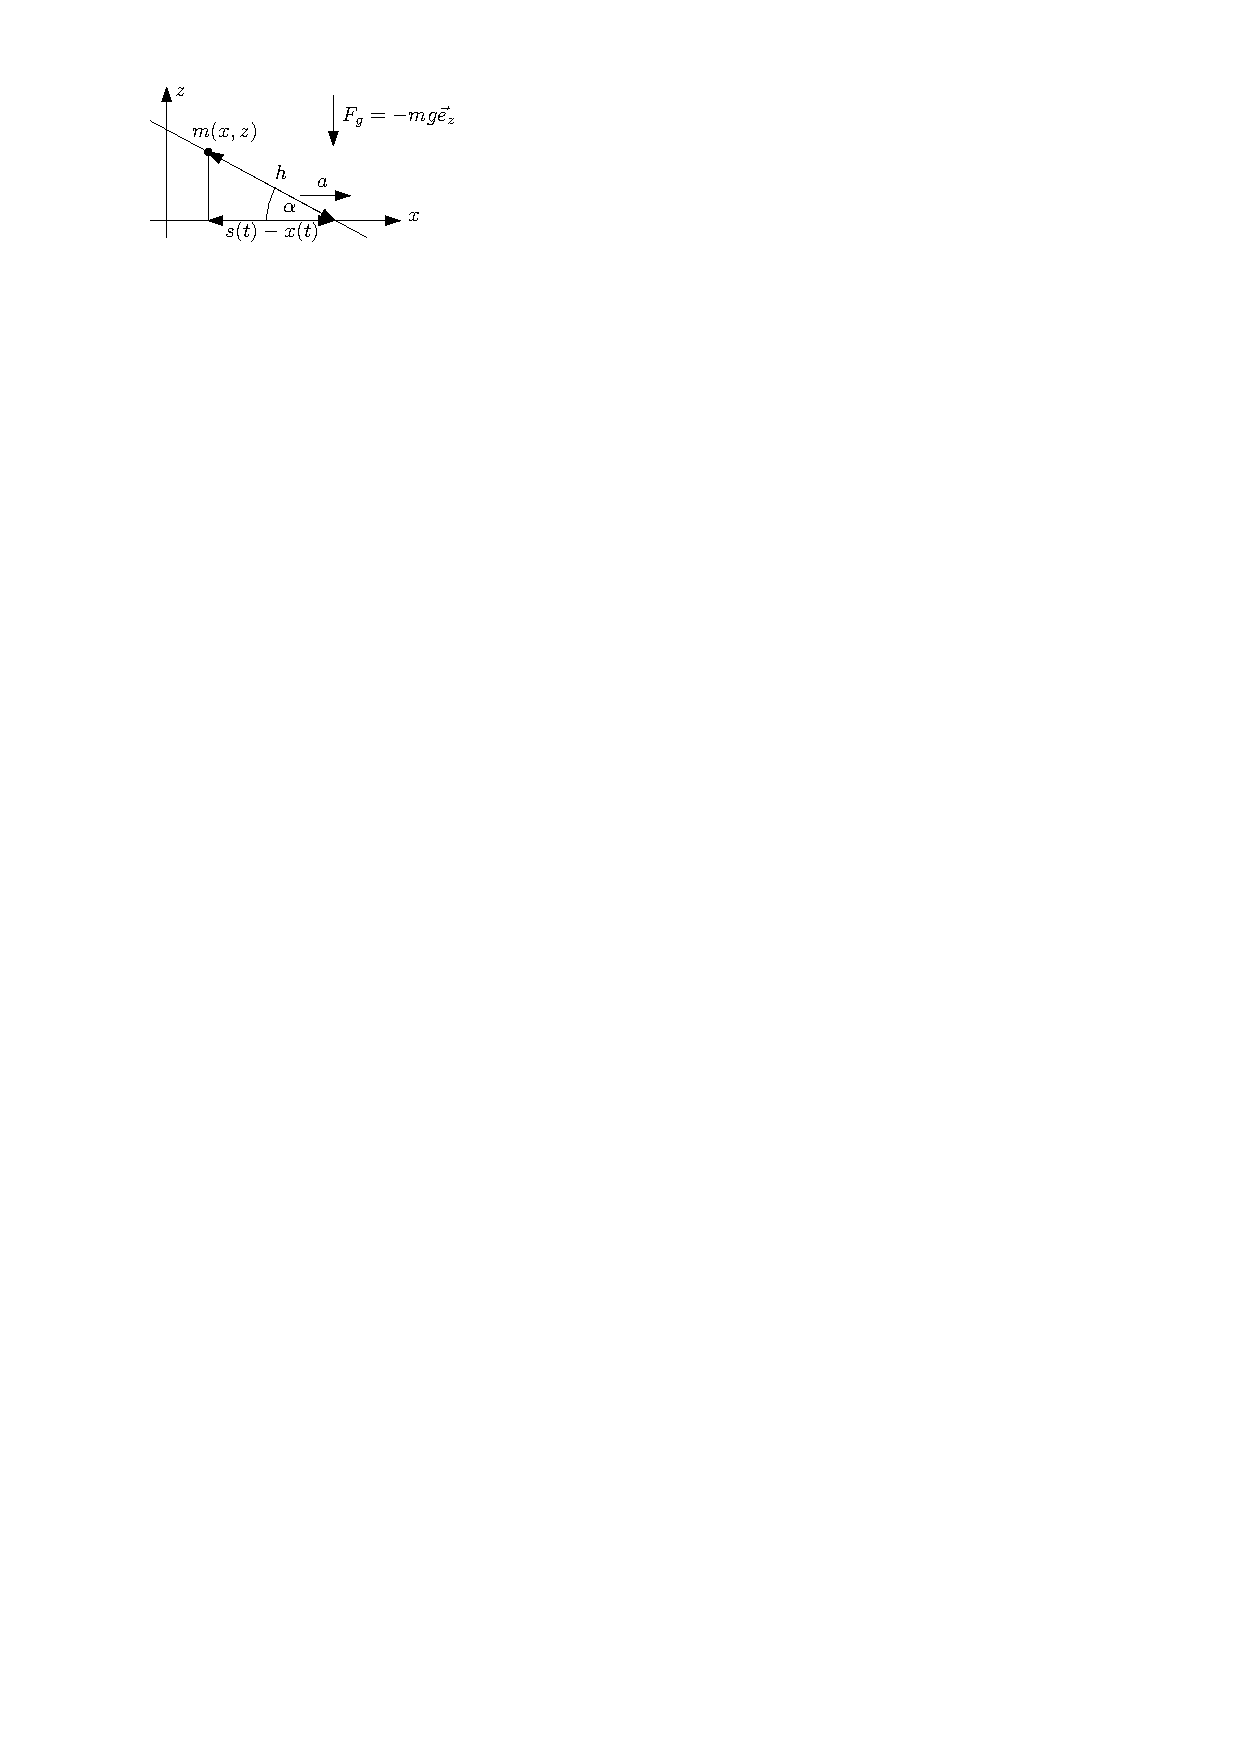
\includegraphics[scale=1.5]{figures/ueb4/aufgabe9}
	\caption{Skizze für die Variablen von Aufgabe 9.}
	\label{fig:ueb4_aufgabe9}
\end{figure}

Es gilt $\sin \alpha = \frac{z(t)}{h}$ und $\cos \alpha = \frac{s(t) - x(t)}{h}$, also
\[
	\frac{z(t)}{\sin \alpha} = \frac{s(t) - x(t)}{\cos \alpha}
	\quad \Longleftrightarrow \quad 
	z(t) \cos(\alpha) = (s(t) - x(t)) \sin \alpha
	\text{.}
\]

Die Zwangsbedingung ist damit $A(x, z, t) = \left( x(t - \underbrace{\frac{1}{2} a t^2}_{= s(t)} \right) \sin(\alpha) + z(t) \cos(\alpha) \overset{!}{=} 0$.

Die Formel für die Zwangskräfte lautet $Z_i(x, z, t) = \lambda \frac{\partial A(x, z, t)}{\partial x_i}$. Damit berechnen wir:
\[
	\mvec{Z_x \\ Z_z} 
	= \mvec{\lambda \frac{\partial A(\cdot)}{\partial x} \\ \lambda \frac{\partial A(\cdot)}{\partial z}}
	= \lambda \mvec{\sin(\alpha) \\ \cos(\alpha)}
	\text{.}
\]

Wie berechnen wir die Lagrange-Multiplier $\lambda$? Ansatz:
\[
	m \mvec{\ddot{x}(t) \\ \ddot{z}(t)} 
	= \mvec{F_x + Z_x \\ F_z + Z_z}
	= \mvec{0 + \lambda \sin(\alpha) \\ -mg + \lambda \cos(\alpha)}
\]
Weiter brauchen wir: 
\begin{align*}
	\frac{\partial A(\cdot)}{\partial t} &= \left( \dot{x}(t) - at \right) \sin(\alpha) + \dot{z}(t) \cos(\alpha) \overset{!}{=} 0 \text{ und } \\
	\frac{\partial A(\cdot)}{\partial t^2} &= \left( \ddot{x}(t) - a \right) \sin(\alpha) + \ddot{z}(t) \cos(\alpha) \overset{!}{=} 0
	\text{.}
\end{align*}
Daraus gewinnen wir $\ddot{z}(t) = - (\ddot{x}(t) - a) \tan(\alpha)$, das wir in obige Kraftgleichung geteilt durch $m$ einsetzen:
\[
	\mvec{\ddot{x}(t) \\ -(\ddot{x}(t) - a) \tan(\alpha)}
	= \mvec{ \frac{\lambda}{m} \sin(\alpha) \\ -g + \frac{\lambda}{m} \cos(\alpha) }
	\quad \Longleftrightarrow \quad 
	\mvec{\ddot{x}(t) \\ \ddot{x}(t)} = \mvec{ \frac{\lambda}{m} \sin(\alpha) \\ a + g \cot(\alpha) - \frac{\lambda}{m}  \cos(\alpha) \cot(\alpha) }
	\text{.}
\]

Nun können wir das $\lambda$ bestimmen, denn es folgt die Bedingung
\begin{align*}
	& \frac{\lambda}{m} \sin(\alpha) = a + g \cot(\alpha) - \frac{\lambda}{m} \cos(\alpha) \cot(\alpha) \\
	\Longleftrightarrow~ & \frac{\lambda}{m} \left( \sin(\alpha) + \frac{\cos^2(\alpha)}{\sin(\alpha)} \right) = a + g \frac{\cos(\alpha)}{\sin(\alpha)} \\
	\Longleftrightarrow~ & \frac{\lambda}{m} \frac{1}{\sin(\alpha)} = a + g \frac{\cos(\alpha)}{\sin(\alpha)} \\
	\Longleftrightarrow~ & \lambda = m ( a \sin(\alpha) + g \cos(\alpha) )	
\end{align*}

Das wieder in die Kraftgleichung geteilt durch $m$ einsetzen:
\[
	\mvec{\ddot{x}(t) \\ \ddot{z}(t)} 
	= \mvec{ (a \sin(\alpha) + g \cos(\alpha)) \sin(\alpha) \\ - g + (a \sin(\alpha) + g \cos(\alpha)) \cos(\alpha)}
	\text{.}
\]

Anfangsbedingungen: $\dot{x}(t = 0) = v_0$ und $x(t = 0) = x_0$. Damit noch $x(t)$ berechnen: 
\begin{align*}
	\dot{x}(t) 
	&= \int_0^t \ddot{x}(t') \md t' + \underbrace{\dot{x}(t = 0)}{= v_0}
	= t \sin(\alpha) (a \sin(\alpha) + g \cos(\alpha) + v_0 \\
	x(t)
	&= \int_0^t \dot{x}(t') \md t' + \underbrace{x(t = 0)}{= x_0}
	= \frac{1}{2} t^2 \sin(\alpha) (a \sin(\alpha) + g \cos(\alpha)) + v_0 t + x_0
\end{align*}
Das fehlende $z(t)$ kann man nun aus $A(x, z, t) = 0$ berechnen:
\[
	z(t) = \frac{1}{2} t^2 \sin(\alpha) (a \cos(\alpha) - g \sin(\alpha)) - (v_0 t + x_0) \tan(\alpha)
	\text{.}
\]

\section*{Aufgabe 10}

Koordinaten sind gegeben durch $\vec{x} = r \mvec{\sin \theta \cos \phi \\ \sin \theta \sin \phi \\ \cos \theta} = \mvec{x \\ y \\ z}$.

Zunächst die Richtungsvektoren berechnen: 
\begin{align*}
	\vec{k}_r &= \frac{\partial \vec{x}}{\partial r} = \mvec{ \sin \theta \cos \phi \\ \sin \theta \sin \phi \\ \cos \theta}, \\
	\vec{k}_\theta &= \frac{\partial \vec{x}}{\partial \theta} = r \mvec{\cos \theta \cos \phi \\ \cos \theta \sin \phi \\ -r \sin \theta}, \\
	\vec{k}_\phi &= \frac{\partial \vec{x}}{\partial \phi} = r \sin \theta \mvec{ - \sin \phi \\ \cos \phi \\ 0}
	\text{.}
\end{align*}

Für die Einheitsvektoren berechnen wir die Länge der Vektoren:
\begin{align*}
	\mabs{\vec{k}_r} &= \sqrt{\vec{k}_r^2} = \sqrt{\sin^2 \theta \cos^2 \phi + \sin^2 \theta \sin^2 \phi + \cos^2 \theta} = \sqrt{\underbrace{\sin^2 \theta \underbrace{(\cos^2 \phi + \sin^2 \phi)}_{ = 1} + \cos^2 \theta}_{= 1}} = 1, \\
	\mabs{\vec{k}_\theta} &= \sqrt{\vec{k}_\theta^2} = \dots = \sqrt{r^2} = r, \\
	\mabs{\vec{k}_\phi} &= \sqrt{\vec{k}_\phi^2} = \sqrt{r^2 \sin^2 \theta (\sin^2 \phi + \cos^2 \phi)} = r \sin \theta
	\text{.}
\end{align*}
Die Einheitsvektoren sind also:
\[
	\vec{e}_r = \mvec{\sin \theta \cos \phi \\ \sin \theta \sin \phi \\ \cos \theta},
	\quad 
	\vec{e}_\theta = \mvec{\cos \theta \cos \phi \\ \cos \theta \sin \phi \\ - \sin \theta},
	\quad 
	\vec{e}_\phi = \mvec{- \sin \phi \\ \cos \phi \\ 0}
	\text{.}
\]

Nun gilt für die zeitliche Ableitung von $x$:
\[
	\mdotvec{x}(t) 
	= \msimplediff{\vec{x}}{t} 
	= \msimplediff{r}{t} \frac{\partial \vec{x}}{\partial r}
	+ \msimplediff{\theta}{t} \frac{\partial \vec{x}}{\partial \theta} 
	+ \msimplediff{\phi}{t} \frac{\partial \vec{x}}{\partial \phi}
	= \dot{r} \vec{e}_r + \dot{\theta} r \vec{e}_\theta + \dot{\phi} r \sin \theta \vec{e}_\phi
	\text{.}
\]

Damit kann man die kinetische Energie wie folgt schreiben:
\[
	T = \frac{1}{2} m \mdotvec{x}^2 = \frac{1}{2} m \left( \dot{r}^2 + r^2 \dot{\theta}^2 + r^2 \sin^2 \theta \dot{\phi}^2 \right)
	\text{.}
\]

Jetzt können wir die Lagrange-Funktion aufschreiben als 
\[
	\mathcal{L} = T - V = \frac{1}{2} m \left( \dot{r}^2 + r^2 \dot{\theta}^2 + r^2 \sin^2 \theta \dot{\phi}^2 \right) - V(r, t)
	\text{.}
\]

Die Lagrange-Funktion hängt also nicht explizit von $\phi$ ab. Also ist $\phi$ eine zyklische Koordinate. Denn eine Koordinate ist zyklisch, wenn $\frac{\partial \mathcal{L}}{\partial \phi} = 0 = \msimplediff{}{} \frac{\partial \mathcal{L}}{\partial \phi}$.

Der Impuls 
\[
	P \phi = \frac{\partial \mathcal{L}}{\partial \dot{\phi}} = mr^2 \sin^2 \theta \dot{\phi} \neq 0
\]
ist daher konstant, erhalten. In diesem Fall ist der Drehimpuls also erhalten.

\textbf{Anmerkung:} Es gilt
\[
	\frac{\partial L}{\partial q} = \msimplediff{}{t} \frac{\partial L}{\partial \dot{q}}
	\text{.}
\]
Wenn jetzt $\frac{\partial L}{\partial q} = 0$, dann ist auch $\msimplediff{}{t} \left( \frac{\partial L}{\partial \dot{q}} \right) = \msimplediff{}{t} Pp = 0$ (also zyklisch, wenn $Pp \neq 0$).
	\chapter{Übung 5}

\section*{Aufgabe 11}

Siehe Abbildung \ref{fig:ueb5_aufgabe11} für eine Skizze mit den Variablen.

\begin{figure}[h]
	\centering
	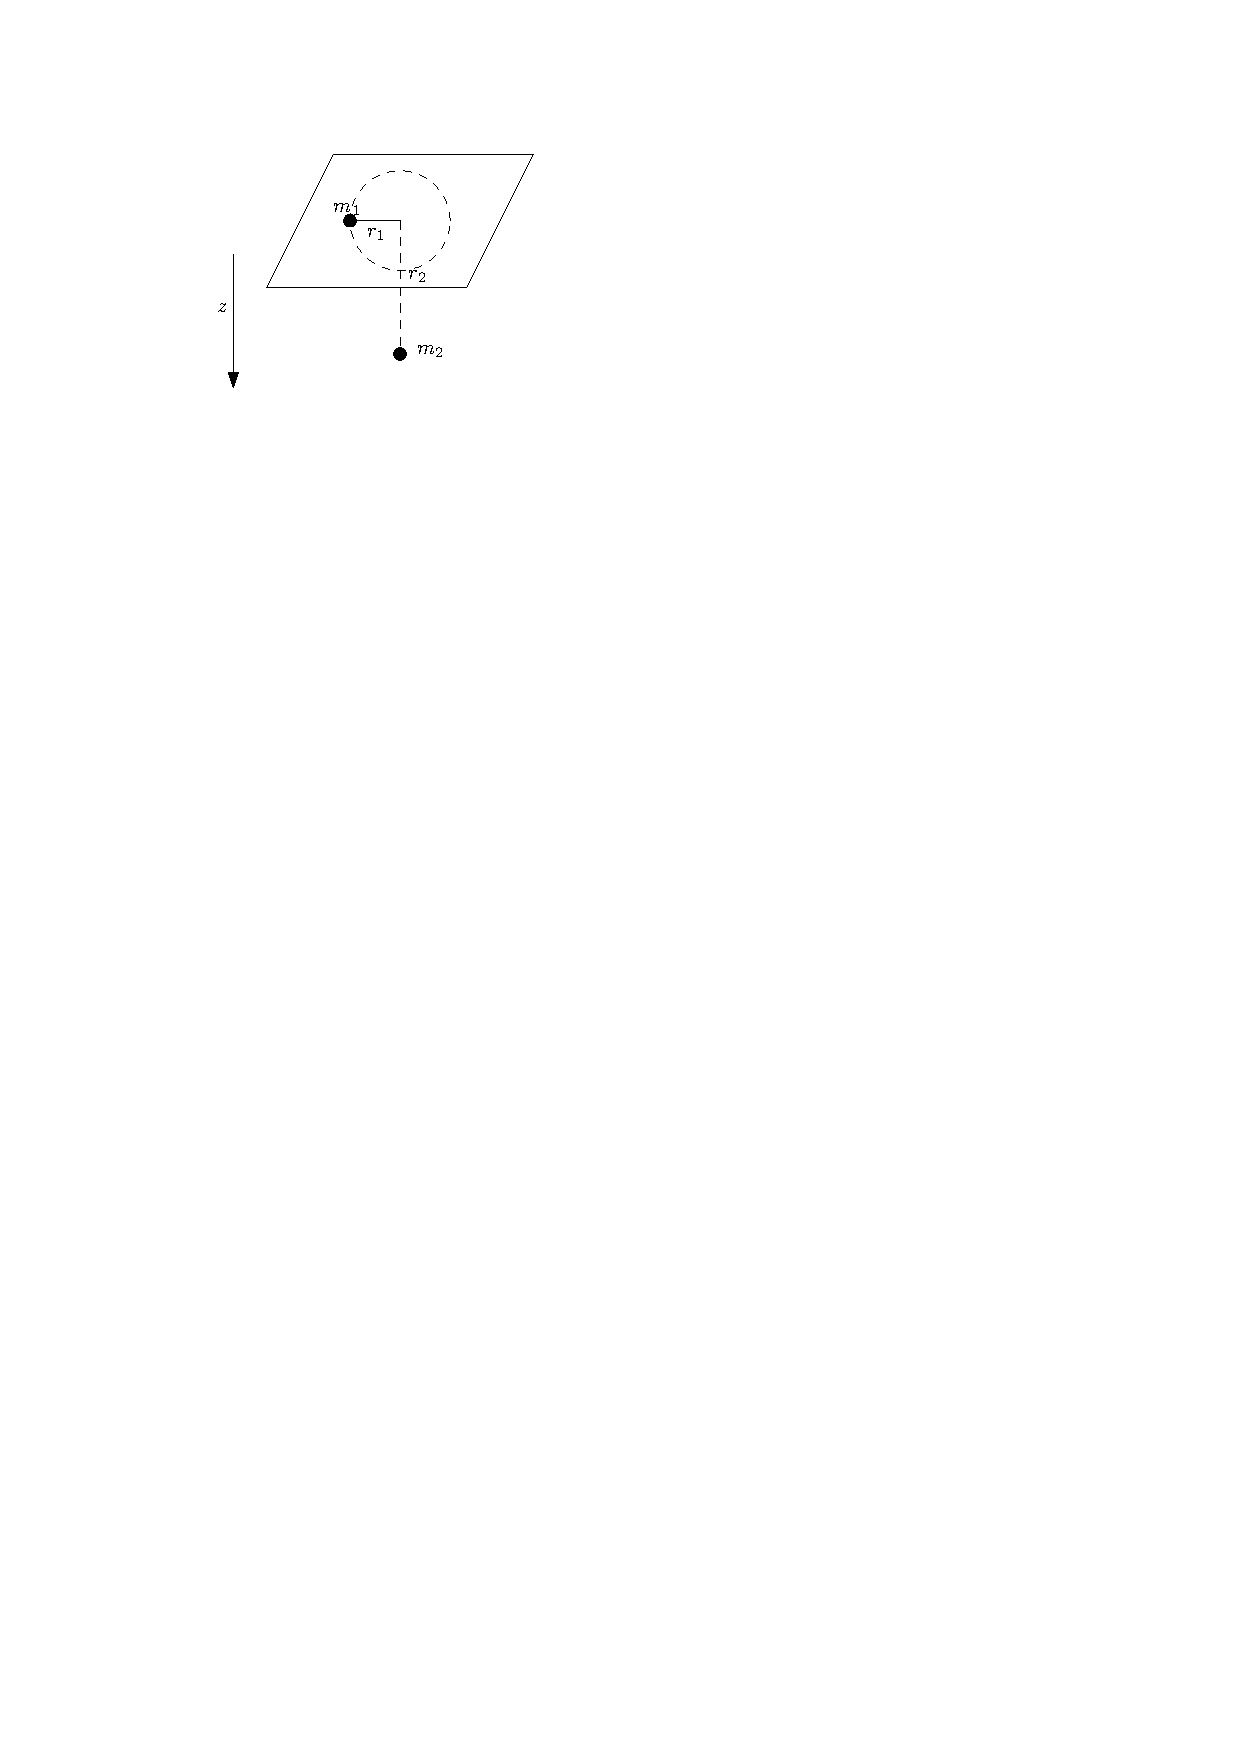
\includegraphics{figures/ueb5/aufgabe11}
	\label{fig:ueb5_aufgabe11}
	\chapter{Skizze von Aufgabe 11. Die Koordinate $z$ zeigt nach unten.}
\end{figure}

Wir wählen als Koordinaten:
\[
	\vec{x}_1 = \mvec{ \cos \phi_1 r_1 \\ \sin \phi_1 r_1 \\ z_1} 
	\quad \text{ und } \quad 
	\vec{x}_2 = r_2 \mvec{ \sin \theta_2 \cos \phi_2 \\ \sin \theta_2 \sin \phi_2 \\ \cos \theta_2 }
	\text{.}
\]

Also $F_g = m g \vec{e}_z = - \vec{\nabla} V_g$ mit $V_g = - m g z$ (auf Vorzeichen achten).

Die Länge vom Seil ist $l = r_1 + r_2$. Also Zwangsbedingung: $A = r_1 + r_2 - l = 0$ und $z_1 = const$. Wähle $z_1 = 0$, dann: $V_{g, 1} = - m_1 g \cdot 0 = 0$.

Damit ist $T_1 = \frac{1}{2} m_1 (\dot{x}_1^2 + \dot{y}_1^2)$, wobei 
\begin{align*}
	\dot{x}_1 &= \dot{r}_1 \cos \phi_1 - r_1 \dot{\phi}_1 \sin \phi_1 \text{ und} \\
	\dot{y}_1 &= \dot{r}_1 \sin \phi_1 + r_1 \dot{\phi}_1 \cos \phi_1 
	\text{.}	
\end{align*}

Also eingesetzt (Rechnung analog zu Aufgabe 10): $T_1 = \frac{1}{2} m_1 \left( \dot{r}_1^2 + r_1^2 \dot{\phi}_1^2 \right)$. Weiterhin 
\[
	T_2 \overset{\text{Aufg. 10}}{=} \frac{1}{2} m_2 \left( \dot{r}_1^2 + r_2^2 \dot{\theta})_2^2 + r_2^2 \dot{\phi}_2^2 \sin^2 \theta_2 \right)
	\text{.}
\]

Ingesamt folgt die Lagrange-Funktion, wobei $r_2 = l - r_1$ und $\dot{r}_2 = \dot{r}_1$ genutzt wird:
\begin{align*}
	L 
	&= T_1 + T_2 - V_1 - V_2 \\
	&= \frac{1}{2} m_1 \left( \dot{r}_1^2 + r_1^2 \dot{\phi}_1^2 \right)
	+ \frac{1}{2} m_2 \left( \dot{r}_2^2 + r_2 ^2 \dot{\theta}_2^2 + r_2^2 \dot{\phi}_2^2 \sin^2 \theta_2 \right)
	+ m g r_2 \cos \theta_2 \\
	&= \frac{1}{2} (m_1 + m_2) \dot{r}_1^2 
	+ \frac{1}{2} m_1 r_1^2 \dot{\phi}_1^2
	+ \frac{1}{2} (l - r_1)^2 (\dot{\theta}_2^2 + \dot{\phi}_2^2 \sin^2 \theta_2)
	+ m_2 g (l - r_1) \cos \theta_2
	\text{.}
\end{align*}

Was sind die zyklischen Koordinaten? Die müssen die Bedingung
\[
	\frac{\partial L}{\partial q_i} = 0 
	\quad \text{ und } \quad 
	\frac{\partial L}{\partial \dot{q}_i} \neq 0
\]
erfüllen.

Erhalten sind 
\begin{align*}
	P \phi_1 &= \frac{\partial L}{\partial \dot{\phi}_1} = m_1 r_1^2 \dot{\phi}_1 \text{ und } \\
	P \phi_2 &= \frac{\partial L}{\partial \dot{\phi}_2} = m_2 (l - r_1)^2 \sin^2 \theta_2 \dot{\phi}_2
	\text{.}
\end{align*}

Jetzt Einschränkung: $\phi_2 = \theta_2 = 0$. Damit vereinfacht sich die Lagrange-Funktion zu 
\[
	L = \frac{1}{2} (m_1 + m_2) \dot{r}_1^2 + \frac{1}{2} m_1 r_1^2 \dot{\phi}_1^2 + m_2 g (l - r_1) = L(r_1, \phi_1)
	\text{.}
\]	
Damit bestimmen wir die Lagrange-Gleichungen:
\begin{align*}
	& \frac{\partial L}{\partial r_1} = \msimplediff{}{t} \frac{\partial L}{\partial \dot{r}_1} \\
	\Longrightarrow~ & m_1 r_1 \dot{\phi}_1^2 - m_2 g = \msimplediff{}{t} \left( (m_1 + m_2) \dot{r}_1 \right) = (m_1 + m_2) \ddot{r}_1 \\
	\Longrightarrow~ & \ddot{r}_1 = \frac{1}{m_1 + m_2} \left( m_1 r_1 \dot{\phi}_1^2 - m_2 g \right) \\
	& \frac{\partial L}{\partial \phi_1} = \msimplediff{}{t} \frac{\partial L}{\partial \dot{\phi}} \\
	\Longrightarrow~ & 0 = \msimplediff{}{t} \left( m_1 r_1^2 \dot{\phi}_1 \right) = 2 m_1 \dot{r}_1 r_1 \dot{\phi}_1 + m_1 r_1^2 \ddot{\phi}_1 \\
	\Longrightarrow~ & \ddot{\phi}_1 = - \frac{2}{r_1} \dot{r}_1 \dot{\phi}_1
	\text{.}
\end{align*}

\section*{Aufgabe 12}

Für eine Skizze mit den Variablen siehe Abbildung \ref{fig:ueb5_aufgabe12}.

\begin{figure}
	\centering
	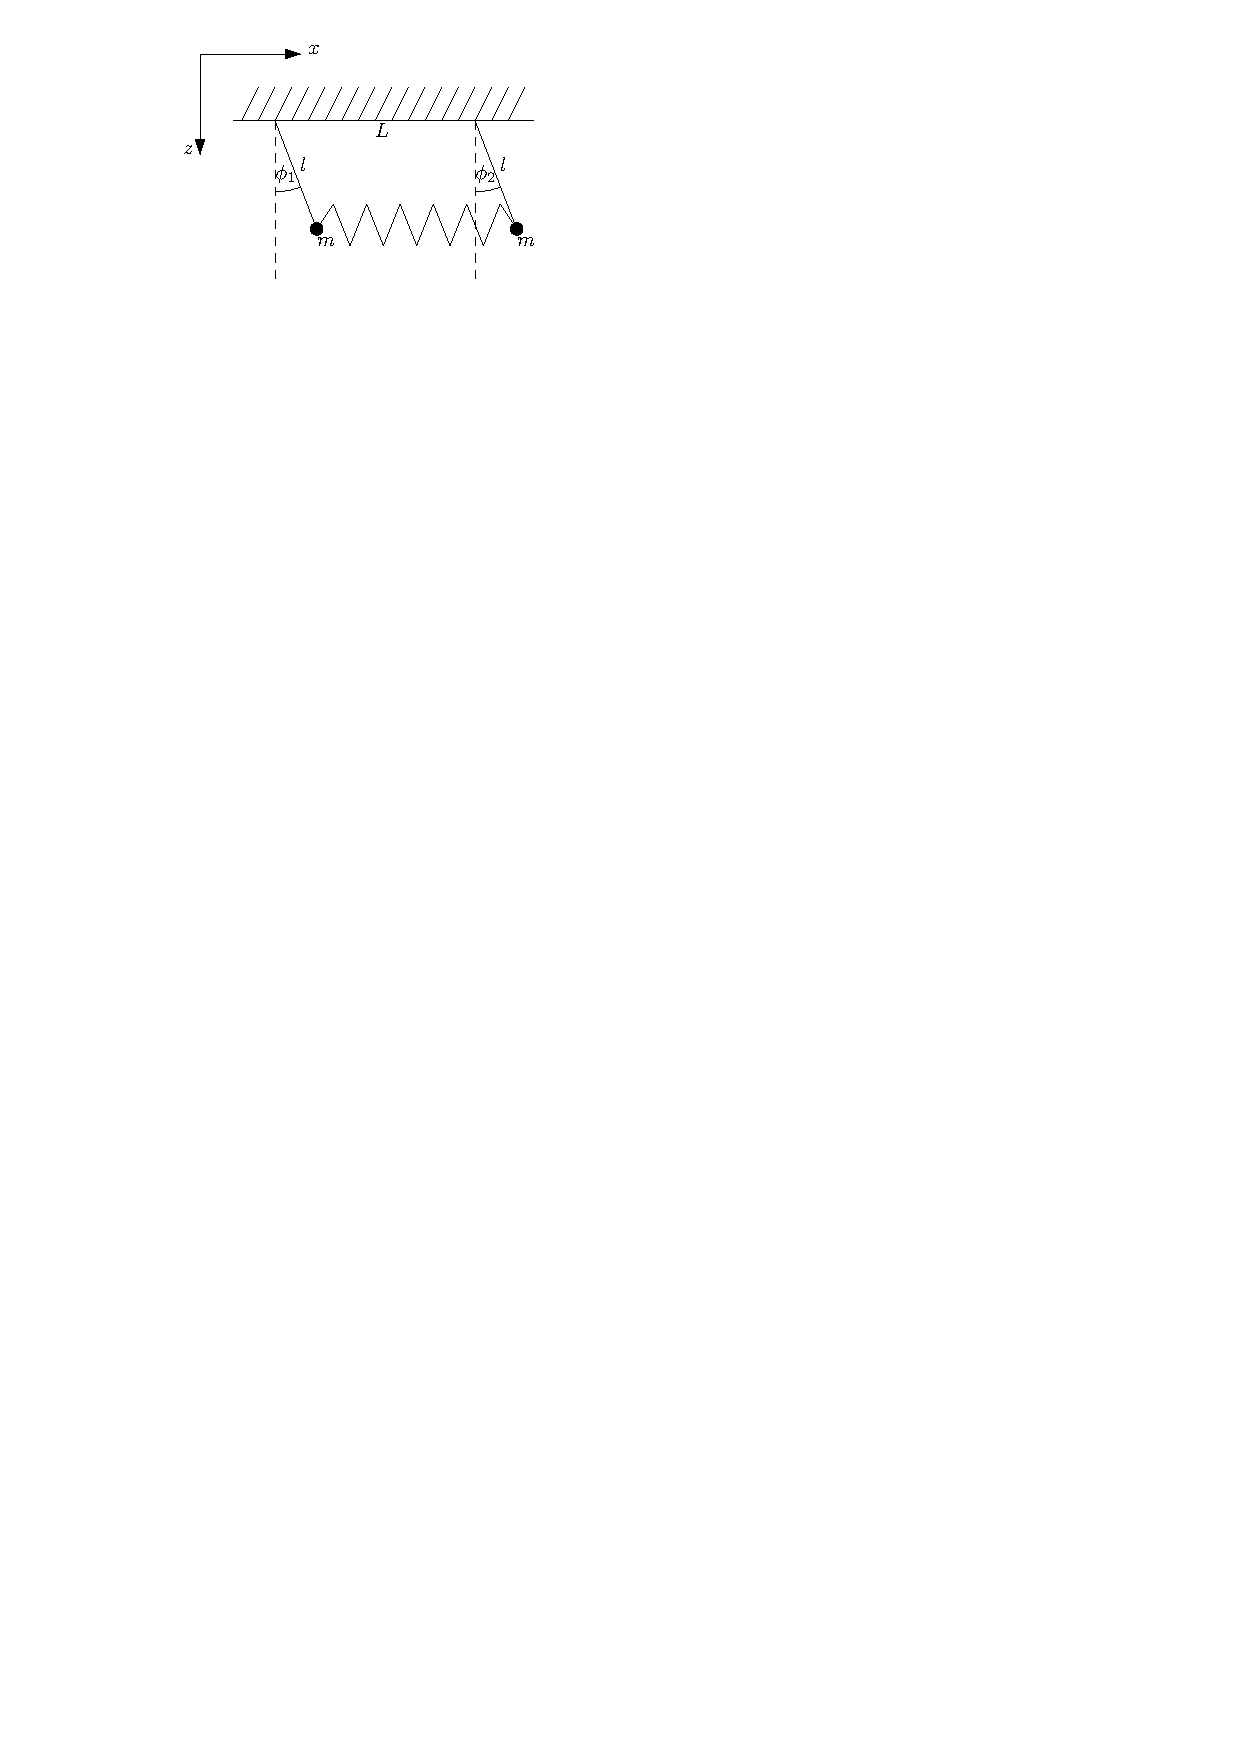
\includegraphics{figures/ueb5/aufgabe12}
	\label{fig:ueb5_aufgabe12}
	\caption{Skizze von Aufgabe 12.}
\end{figure}

Es gilt also:
\[
	x_1 = l \sin \phi_1,
	\quad 
	z_1 = l \cos \phi_1,
	\quad 
	x_2 = l \sin \phi_2 + L
	\quad \text{ und } \quad 
	z_2 = l \cos \phi_2
	\text{.}
\]

Damit folgen die Ableitungen
\begin{align*}
	\dot{x}_1 &= \dot{\phi}_1 l \cos \phi_1, \\
	\dot{x}_2 &= \dot{\phi}_2 l \cos \phi_2, \\
	\dot{z}_1 &= - l \dot{\phi}_1 \sin \phi_1 \text{ und } \\
	\dot{z}_2 &= - l \dot{\phi}_2 \sin \phi_2
	\text{.}
\end{align*}

Die Energien sind
\begin{align*}
	T &= \frac{1}{2} m \left( \dot{x}_1^2 + \dot{z}_1^2 \right)
	+ \frac{1}{2} m \left( \dot{x}_2^2 + \dot{z}_2^2 \right)	
	= \frac{1}{2} m l^2 \left( \dot{\phi}_1^2 + \dot{\phi}_2^2 \right), \\
	V_g &= \sum_{i = 1, 2} - m g z_i = - m g l (\cos \phi_1 + \cos \phi_2) \text{ und } \\
	V_F &= \frac{1}{2} \kappa (x_1 - (x_2 - L))^2 = \frac{1}{2} \kappa l^2 (\sin \phi_1 - \sin \phi_2)^2
\end{align*}
und die Lagrange-Funktion damit
\[
	L = \frac{1}{2} m l^2 (\dot{\phi}_1^2 + \dot{\phi}_2^2)
	- \frac{1}{2} \kappa l^2 (\sin \phi_1 - \sin \phi_2)^2
	+ m g l (\cos \phi_1 + \cos \phi_2)
	\text{.}
\]

Für kleine Auslenkungen approximieren wir mit Taylor:
\begin{align*}
	\sin(x) &= x + \mathcal{O}(x^2) \text{ und } \\
	\cos(x) &= 1 - \frac{x^2}{2} + \mathcal{O}(x^3) = 1 + \mathcal{O}(x^2)
	\text{.}
\end{align*}

Damit vereinfacht sich die Lagrange-Funktion zu
\[
	L = \frac{1}{2} m l^2 (\dot{\phi}_1^2 + \dot{\phi}_2^2)
	- \frac{1}{2} \kappa (\phi_1 - \phi_2)^2
	+ m g l \left( 2 - \frac{\phi_1^2}{2} - \frac{\phi_2^2}{2} \right)
	\text{.}
\]

Jetzt wieder die Lagrange-Gleichungen aufstellen:
\begin{align*}
	\msimplediff{}{t} \frac{\partial L}{\partial \dot{\phi}_1} &= m l^2 \ddot{\phi}_1, \\
	\msimplediff{}{t} \frac{\partial L}{\partial \dot{\phi}_2} &= m l^2 \ddot{\phi}_2, \\
	\frac{\partial L}{\partial \phi_1} &= - \kappa l^2 (\phi_1 - \phi_2) - m g l \phi_1 \text{ und } \\
	\frac{\partial L}{\partial \phi_2} &= \kappa l^2 (\phi_1 - \phi_2) - m g l \phi_2
	\text{.}
\end{align*}

Es folgen daraus die Differentialgleichungen
\[
	\ddot{\phi}_1 = - \frac{\kappa}{m} (\phi_1 - \phi_2) - \frac{g}{l} \phi_1
	\quad \text{ und } \quad 
	\ddot{\phi}_2 = \frac{\kappa}{m} (\phi_1 - \phi_2) - \frac{g}{l} \phi_2
	\text{.}
\]

Mit dem Hinweis:
\begin{align*}
	\ddot{\phi}_2 - \ddot{\phi}_1 &= 2 \frac{\kappa}{m} (\phi_2 - \phi_1) - \frac{g}{l} (\phi_2 - \phi_1), \\
	\underbrace{(\dot{\phi}_2 - \dot{\phi}_1)}_{= \dot{\Phi}_1} &= \left( 2 \frac{\kappa}{m} - \frac{g}{l} \right) \underbrace{\left( \phi_2 - \phi_1 \right)}_{= \Phi_1} \text{ und } \\
	\underbrace{(\dot{\phi}_1 + \dot{\phi}_2)}_{= \dot{\Phi}_2} &= - \frac{g}{l} \underbrace{(\phi_1 + \phi_2)}_{= \Phi_2} \text{.}
\end{align*}

\begin{description}
	\item[Gleichschwingung] $\phi_2 = \phi_1$ $\Longrightarrow$ $\Phi_1 = 0$
	\item[Gegenschwingung] $\phi_2 = -\phi_1$ $\Longrightarrow$ $\Phi_2 = 0$ 
\end{description}

Nun ans Lösen: Wähle den Ansatz 
\[
	\Phi_1(t) = A_1 \cos (\omega_1 t + \beta_1) 
	\quad \text{ und } \quad 
	\Phi_2(t) = A_2 \cos (\omega_2 t + \beta_2)
	\text{.}
\]

Das impliziert $\omega_1^2 = \frac{g}{l} - 2 \frac{\kappa}{m} = \frac{g}{l} \left( 1 - 2 \frac{\kappa}{g} \frac{l}{m} \right)$ und weiter $\omega_2^2 = \frac{g}{l}$. Die anderen Unbekannten bestimmen wir mit den Anfangsbedingungen:
\[
	\phi_1(t = 0) = A
	\quad \text{ und } \quad 
	\phi_2(t = 0) = 0
	\text{.}
\]

Damit $\Phi_1(t = 0) = \phi_1(t = 0) = -A$ und $\Phi_2(t = 0) = - \phi_2(t = 0) = A$. Weiter mit der Anfangsbedingung $\dot{\phi}_1(t = 0) = \dot{\phi}_2(t = 0) = 0$: 
\begin{align*}
	\dot{\Phi}_1(t = 0) &= 0 
	= - A_1 \omega_1 \sin (\omega_1 \cdot 0 + \beta_1) 
	= - A_1 \omega_1 \sin(\beta_1) \text{ und } \\
	\dot{\Phi}_2(t = 0) &= 0 
	= -A_2 \omega_2 \sin(\beta_2) \text{.}
\end{align*}
Also $\beta_1 = \beta_2 = 0$. Zuletzt $\ddot{\Phi}_1(t = 0) = A_1 = A$ und $\ddot{\Phi}_2(t = 0) = A_2 = A$ (wirklich $\ddot{\Phi}$?) 

Am Ende soll folgen: 
\[
	\Phi_1(t) = A \cos (\omega_1 t) 
	\quad \text{ und } \quad 
	\Phi_2(t) = A \cos (\omega_2 t)
	\text{.}
\]

Ergebnis:
\begin{align*}
	\phi_1(t) &= \frac{1}{2} (- \Phi_1 + \Phi_2) = \frac{1}{2} A (\cos(\omega_2 t) - \cos(\omega_1 t)) \text{ und } \\
	\phi_2(t) &= \frac{1}{2} (\Phi_1 + \Phi_2) = \frac{1}{2} A (\cos(\omega_1 t) + \cos (\omega_2 t))
	\text{.}
\end{align*}

Darauf kann man noch die Additionstheoreme $\cos x + \cos y = 2 \cos \left( \frac{x + y}{2} \right) \cos \left( \frac{x - y}{2} \right)$ und $\cos x - \cos y = - 2 \sin \left( \frac{x + y}{2} \right) \sin \left( \frac{x - y}{2} \right)$ anwenden:
\begin{align*}
	\phi_2(t) &= A \cos \left( \frac{\omega_1 + \omega_2}{2} t \right) \cos \left( \frac{\omega_2 - \omega_1}{2} t \right) \\
	\phi_1(t) &= - \underbrace{A \sin \left( \frac{\omega_1 + \omega_2}{2} t \right)}_{= A(t)} \sin \left( \frac{\omega_2 - \omega_1}{2} t \right)
\end{align*}

Interpretation: Die Amplitude ist auch von der Zeit abhängig; wenn die Amplitude von $\phi_2$ am größten ist, ist die Amplitude von $\phi_1$ am kleinsten. Das kann man sich auf \url{http://www.leifiphysik.de/mechanik/kopplung-von-schwingungen/versuche/gekoppelte-pendel-simulation} anschauen.

	\chapter*{Übung 6}

\section*{Aufgabe 13}

Abrollender Kreis mit Mittelpunkt $M(t r_0 | r_0)$. Dann $x(t) = r_0 (t - \cos (t + \phi_x))$ und $y(t) = r_0(1 - \cos(t + \phi_y))$. Da $x(t = 0) \overset{!}{=} 0$ folgt $\phi_x = -\frac{\pi}{2}$ und da $y(t = 0) = 0$ folgt $\phi_y = 0$. Also ist die Parametisierung: $\vec{r}(t) = \mvec{r_0 (t - \sin t) \\ r_0 (1 - \cos t)}$; alles sofern sich der Kreis mit $v = 1 \frac{m}{s}$ bewegt; ansonsten verändert sich der Mittelpunkt entsprechend. Oder man spricht bei $t$ von irgendeinem Parameter $t$ und nicht von der Zeit. 

Bei einer Spiegelung kommt ein Minus vor die $y$-Komponente: $\vec{r}(t) = \mvec{r_0 (t - \sin t) \\ - r_0 (1 - \cos t)}$. Diese Kurve beschreibt die (eine?) Brachistochrone.

\section*{Aufgabe 14}

Zu minimieren ist, wie angegeben: $V(y(x)) = \int \md s \frac{m}{L} g y(x)$. Vereinfachung, da $m$, $L$ und $g$ konstant sind: $\hat{V}(y(x)) = \int \md s y(x)$. Wenn $\hat{V}(y(x))$ minimal ist, dann ist auch $V(y(x))$ minimal.

Wir schreiben 
\[
	\md s 
	= \sqrt{\md x^2 + \md y^2} 
	= \sqrt{\md x^2 + \left( \frac{\md y}{\md x} \md x \right)^2} 
	= \sqrt{(1 + y'^2(x)) \md x^2}
	= \sqrt{1 + y'^2(x)} \md x
	\text{.}
\]

Man kann schreiben:
\[
	L = \int^a_{-a} \md x \frac{L}{2a} = \int \md s = \int^a_{-a} \md x \sqrt{1 + y'^2(x)}
	\text{.}
\]

Daraus folgt gerade die Nebenbedingung (alles rechts von $\md x$ gehört zum Integral!)
\[
	h(y(x)) = \int^a_{-a} \md x \sqrt{1 + y'^2(x)} - \frac{L}{2a} \left( = 0 \right)
	\text{.}
\]

Wir erhalten das Funktional
\[
	S(y(x), \lambda) = \hat{V}(y(x)) + \lambda h(y(x)),
\]
und dafür gilt $\frac{\md S}{\md \lambda} h(y(x)) \overset{!}{=} 0$. Einsetzen:
\begin{align*}
	S(y(x)) &= \int^a_{-a} \md x y(x) \sqrt{1 + y'^2(x)} + \lambda \left( \sqrt{1 + y'^2(x)} - \frac{L}{2a} \right) \\
	&= \int^a_{-a} \md x \sqrt{1 + y'^2(x)} \left( y(x) + \lambda \right) - \lambda \frac{L}{2a}
	\text{.}
\end{align*}

Jetzt führen wir die Substitution $f(x) = y(x) + \lambda$ ein (beachte: $f'(x) = y'(x)$). Damit kann man umschreiben:
\[
	S = \int^a_{-a} \md x \underbrace{\sqrt{1 + f'^2(x)} f(x) - \frac{L}{2a} \lambda}_{= S'}
	\text{.}
\]

Nun gilt es, folgende Euler-Lagrange-Gleichung zu lösen:
\[
	\frac{\partial S'}{\partial f(x)} = \msimplediff{}{x} \frac{\partial S'}{\partial f'(x)}
\]

Wenn man die Ableitungen bestimmt einsetzt und weite ableitet, erhält man:
\begin{align*}
	\sqrt{1 + f'^2(x)} 
	&= \msimplediff{}{x} \left( \frac{\lambda f(x) f'(x)}{\lambda \sqrt{1 + f''^2(x)}} \right) \\
	&= \frac{(f'^2(x) + f(x) f''(x)) \sqrt{1 + f'^2(x)} - f(x) f'(x) \frac{f'(x) f''(x)}{\sqrt{1 + f'^2(x)}}}{1 + f'^2(x)} \\
	&= (1 + f'^2(x))^{-3/2} \cdot \left( f'^2(x) + f(x) f''(x) + f'^4(x) + f(x) f'^2(x) f''(x) - f(x) f'^2(x) f''(x) \right)
	\text{.}
\end{align*}

Den Teiler auf die andere Seite ziehen und ausmultiplizieren:
\[
	(1 + f'^2(x))^2 = 1 + 2 f'^2(x) + f'^4(x) = f'^2(x) + f(x) f''(x) + f'^4(x)
	\text{.}
\]

Nun noch beides auf eine Seite und man erhält $f'^2(x) - f(x) f''(x) + 1 = 0$.

Wir verfolgen den Hinweis und berechnen
\[
	\left( \frac{f''(x)}{f(x)} \right)' = \frac{f'''(x) f(x) - f'(x) f''(x)}{f^2(x)}
\]
sowie die Ableitung der Differentialgleichung
\begin{align*}
	&~ 2f'(x) f''(x) - f'(x) f''(x) - f(x) f'''(x) = 0 \\
	\Longleftrightarrow &~ f'(x) f''(x) - f(x) f'''(x) = 0 = -f^2(x) \left( \frac{f''(x)}{f(x)} \right)' = 0
	\text{.}
\end{align*}

Mit der Annahme $f(x) = 0$:
\[
	\Longleftrightarrow \left( \frac{f''(x)}{f(x)} \right)' = 0 \Longleftrightarrow \frac{f''(x)}{f(x)} = C = \text{const}. \Longleftrightarrow f''(x) = C f(x)
	\text{.}
\]

Einsetzen von $f(x) = C_{\lambda_f} e^{\lambda_f x}$ liefert $\lambda_f^2 = C$ und damit 
\[
	f(x) = C_1 e^{\sqrt{C}x} + C_2 e^{-\sqrt{C} x} = f(-x)
	\text{,}
\]
denn $f$ ist achsensymmetrisch. Daraus folgt $C_1 = C_2$, also 
\[
	f(x) = C_1 \left( e^{\sqrt{C} x} + e^{- \sqrt{C} x} \right) = 2 C_1 \cosh (\sqrt{C} x)
	\text{.}
\]

Nun fehlt noch: $y(x) = 2 C_1 \cosh(\sqrt{C} x) - \lambda$.

Wie bestimmt man $C_1$ und $C$? Es muss $y(a) = 0 = y(-a)$, $y'(0) = 0$ sowie $L = \int^a_{-a} \md x \sqrt{1 + y'^2(x)}$ gelten. Mit diesen drei Gleichungen kann man die noch freien Variablen bestimmen.
	\chapter*{Übung 7}

\section*{Aufgabe 15}

Die Lagrangefunktion ist gegeben durch
\[
	\mathcal{L}(\vec{r}_1, \vec{r}_2, \mdotvec{r}_1, \mdotvec{r}_2) 
	= \frac{m_1}{2} \mdotvec{r}_1^{\,2} + \frac{m_2}{2} \mdotvec{r}_2^{\,2} - U(\mabs{\vec{r}_1 - \vec{r}_2})
	\text{.}
\]

Aus den gegebenen generalisierten Koordinaten (wobei $M = m_1 + m_2$) $\vec{r} = \vec{r}_1 - \vec{r}_2$ und $\vec{R} = \frac{m_1}{M} \vec{r}_1 + \frac{m_2}{M} \vec{r}_2$ folgert man
\begin{align*}
	\vec{r}_1 
	&= \frac{m_1}{M} \vec{r}_1 + \frac{m_2}{M} \vec{r}_1 
	= \vec{R} - \frac{m_2}{M} \vec{r}_2 + \frac{m_2}{M} \vec{r}_1
	= \vec{R} - \frac{m_2}{M} \vec{r} 
	\text{,} \\
	\vec{r}_2 
	&= \frac{m_1}{M} \vec{r}_2 + \frac{m_2}{M} \vec{r}_2
	= \frac{m_1}{M} \vec{r}_2 + \vec{R} - \frac{m_1}{M} \vec{r}_1
	= \vec{R} - \frac{m_1}{M} \vec{r}
	\text{.}
\end{align*}

Die Lagrangefunktion ist nun
\begin{align*}
	\mathcal{L}(\vec{r}, \vec{R}, \mdotvec{r}, \mdotvec{R})
	&= \frac{m_1}{2} \left( \mdotvec{R}^2 + \frac{2 m_2}{M} \mdotvec{r} \mdotvec{R} + \frac{m_2^2}{M^2} \mdotvec{r}^{\,2} \right)	
	+ \frac{m_2}{2} \left( \mdotvec{R}^2 - \frac{2 m_1}{M} \mdotvec{r} \mdotvec{R} + \frac{m_1^2}{M^2} \mdotvec{r}^{\,2} \right)
	- U(\mabs{\vec{r}}) \\
	&= \frac{M}{2} \mdotvec{R}^2 + \frac{m_1 m_2 (m_1 + m_2)}{2 M^2} \mdotvec{r}^{\,2} - U(\mabs{\vec{r}}) \\
	&= \frac{M}{2} \mdotvec{R}^2 + \frac{\mu}{2} \mdotvec{r}^{\,2} - U(\mabs{\vec{r}})
	\text{,}
\end{align*}
wobei $\mu = \frac{m_1 m_2}{M}$.

(TODO (ii))

Nun sind die generalisierten Koordinaten $\vec{r} = \vec{r}_1 - \vec{r}_2$ und $\vec{\rho} = \vec{r}_1 + \vec{r}_2$. Wieder drücken wir $\vec{r}_1$ und $\vec{r}_2$ durch die generalisierten Koordinaten aus:
\[
	\vec{r}_1 = \frac{\vec{r} + \vec{\rho}}{2}
	\quad \text{ und } \quad 
	\vec{r}_2 = \frac{\vec{\rho} - \vec{r}}{2}
	\text{.}
\]

Damit ergibt sich dann folgende Lagrangefunktion:
\begin{align*}
	\mathcal{L}(\vec{r}, \vec{\rho}, \mdotvec{r}, \mdotvec{\rho})
	&= \frac{m_1}{8} (\mdotvec{\rho}^{\,2} + \mdotvec{r}^{\,2} + 2 \mdotvec{r} \mdotvec{\rho})
	+ \frac{m_2}{8} (\mdotvec{\rho}^{\,2} + \mdotvec{r}^{\,2} - 2 \mdotvec{r} \mdotvec{\rho})
	- U(\mabs{\vec{r}}) \\
	&= \frac{M}{8} (\mdotvec{\rho}^{\,2} + \mdotvec{r}^{\,2}) + \underbrace{\frac{m_1 - m_2}{4} \mdotvec{r} \mdotvec{\rho}}_{\text{führt zu gekoppelter DGL}} - U(\mabs{\vec{r}})	
	\text{.}
\end{align*}

\section*{Aufgabe 16}

\subsection*{a)}
\begin{itemize}
	\item $T = \frac{1}{2} m \mdotvec{q}^{\,2}$
	\item $\mathcal{L} = \frac{1}{2} m (\dot{x}_1^2 + \dot{x}_2^2 + \dot{x}_3^2) - V(x_1, x_2, x_3)$
	\item $p_i = \frac{\partial \mathcal{L}}{\partial \dot{x}_i}$
	\item $p_1 = m \dot{x}_1$
	\item $p_2 = m \dot{x}_2$
	\item $p_3 = m \dot{x}_3$
\end{itemize}

\subsection*{b)}
\begin{itemize}
	\item $\dot{x}_i = \frac{p_i}{m}$
	\item $\mdotvec{x} = \frac{\vec{p}}{m}$
	\item $T(\vec{p}) = \frac{p_1^2 + p_2^2 + p_3^2}{2m} = \frac{\vec{p}^2}{2 m}$
\end{itemize}

\subsection*{c)}
\begin{itemize}
	\item $H = T(\vec{p}) + V(\vec{q}) 
		= \mdotvec{q} \, \vec{p} - L
		= \frac{\vec{p}^{\,2}}{m} \left( \frac{\vec{p}^{\,2}}{2 m} - V(\vec{x}) \right)
		= \frac{\vec{p}^{\,2}}{2 m} + V(\vec{x})$
	\item $\dot{x}_i = \frac{\partial H(\vec{x}, \vec{p})}{\partial p_i} = \frac{\partial T(\vec{p})}{\partial p_i} = \frac{p_i}{m}$
	\item $- \dot{p}_i = \frac{\partial H(\vec{x}, \vec{p})}{\partial x_i} = \frac{\partial V(\vec{x})}{\partial x_i}$ $\Longleftrightarrow$ $\dot{p}_i = - \frac{\partial V(\vec{x})}{\partial x_i}$ $\Longrightarrow$ $\ddot{x}_i = \frac{\dot{p}_i}{m} = - \frac{1}{m} \frac{\partial V(\vec{x})}{\partial x_i}$
	\item $F_i = m \ddot{x}_i = - \frac{\partial V}{\partial x_i}$
	\item $\vec{F}_i = - \nabla V(\vec{x})$
	\item Euler-Lagrange-Gleichung:
	\begin{align*}
		& \msimplediff{}{t} \left( \frac{\partial \mathcal{L}(\vec{x}, \mdotvec{x})}{\partial \dot{x}_i} \right) - \frac{\partial \mathcal{L}(\vec{x}, \mdotvec{x}}{\partial x_i} 
		= \msimplediff{}{t} \left( \frac{\partial T(\mdotvec{x})}{\partial \dot{x}_i} \right) + \frac{\partial V(\vec{x})}{\partial x_i} 
		= \msimplediff{}{t}	(m \dot{x}_i) + \frac{\partial V(\vec{x})}{\partial x_i} = 0 \\
		\Longleftrightarrow &~ \ddot{x}_i = - \frac{1}{m} \frac{\partial V(\vec{x})}{\partial x_i}
	\end{align*}

\end{itemize}
	\chapter*{Übung 8}

\section*{Aufgabe 17}

Für eine Skizze der Aufgabe mit den Koordinaten siehe Abbildung \ref{fig:ueb8_aufgabe17}.

\begin{figure}[h]
	\centering
	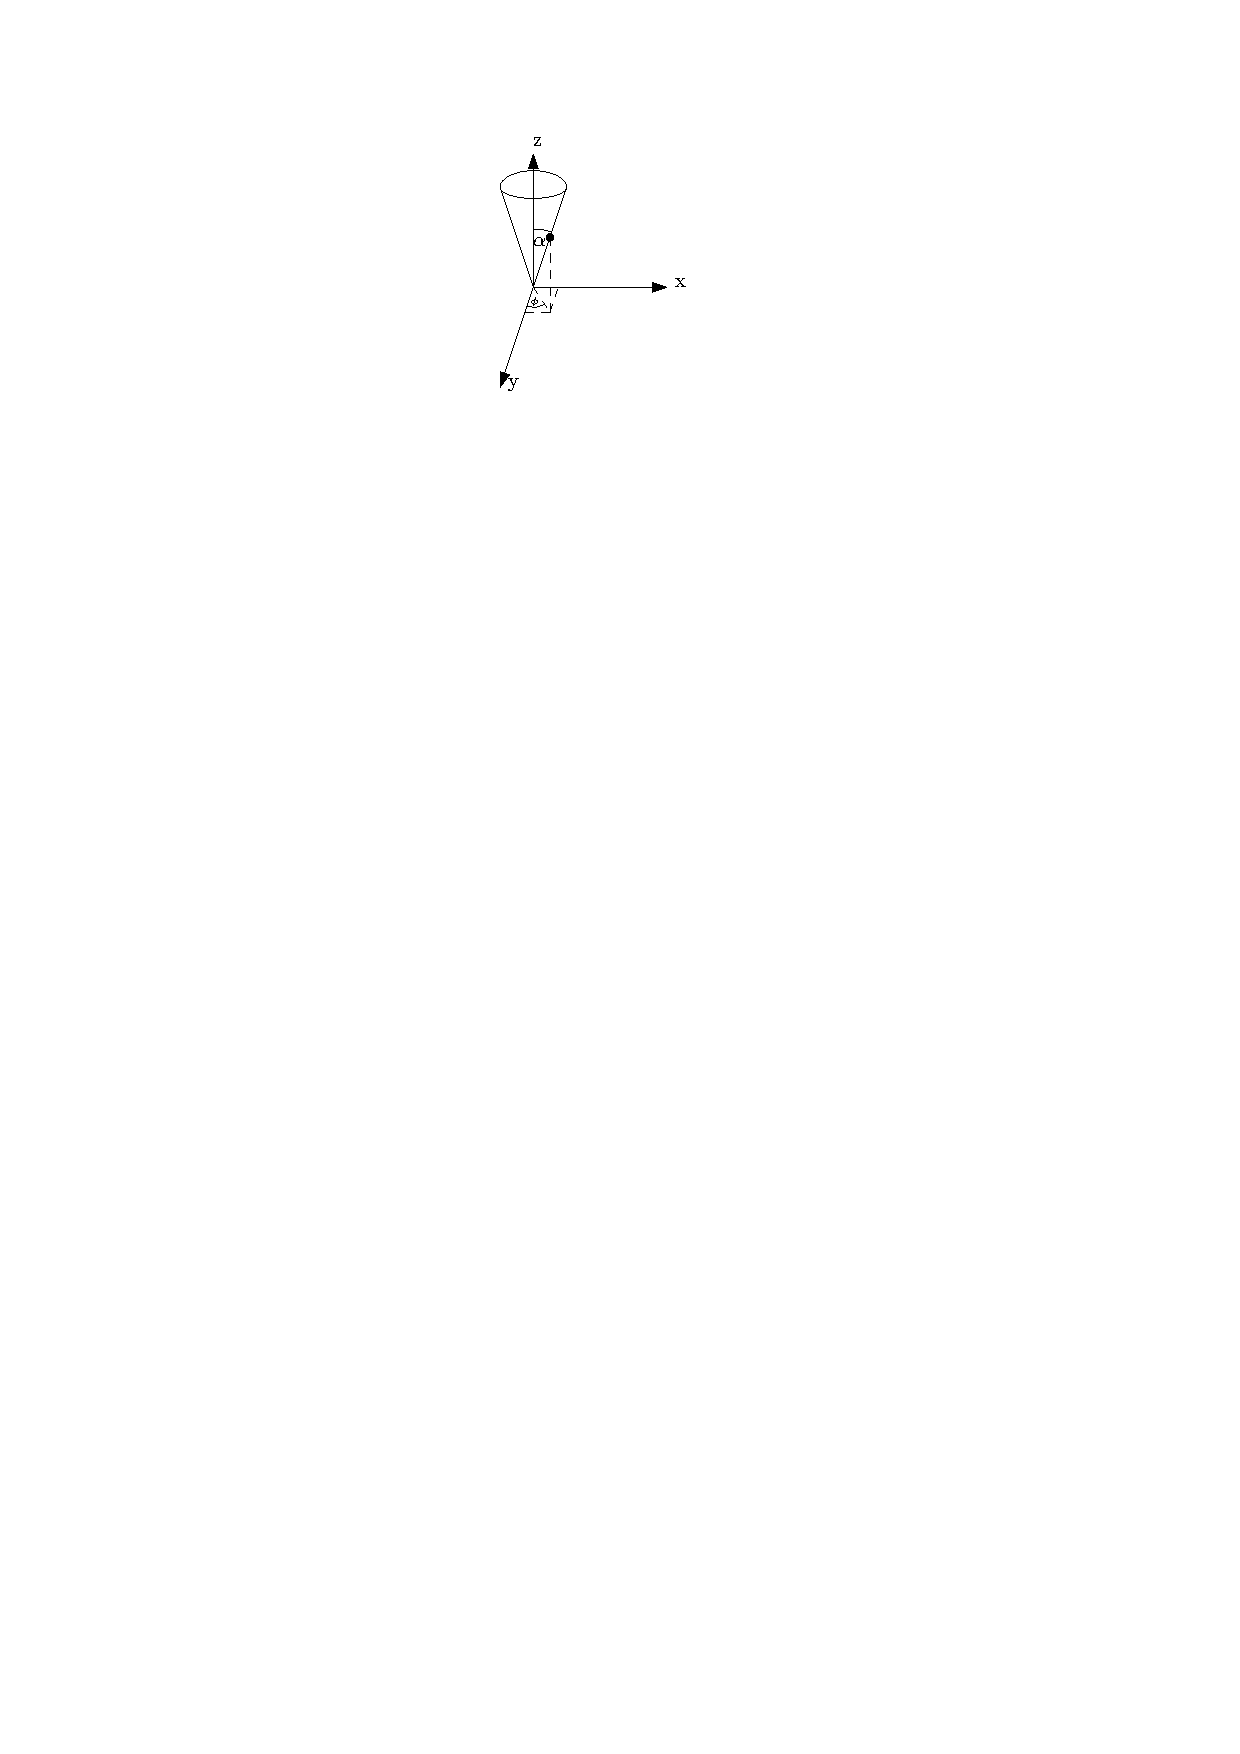
\includegraphics{figures/ueb8/aufgabe17}
	\caption{Skizze von Aufgabe 17 mit eingezeichneten Koordinaten.}
	\label{fig:ueb8_aufgabe17}
\end{figure}

Der Abstand der Masse zur $z$-Achse ist $r = \sqrt{x^2 + y^2}$ und der Zusammenhang zwischen Abstand und $z$-Koordinate ist $\tan(\alpha) = \frac{r}{z}$. Also ist die Zwangsbedingung $0 = \frac{\sqrt{x^2 + y^2}}{\tan(\alpha)} - z$.

Mit $r = z \tan(\alpha)$ ist dann
\begin{align*}
	x &= \sin(\phi) z \tan(\alpha) \text{,} \\
	y &= \cos(\phi) z \tan(\alpha) \text{,} \\
	\dot{x} &= \tan(\alpha) (\cos(\phi) \dot{\phi} z + \sin(\phi) \dot{z}) \text{,} \\
	\dot{y} &= \tan(\alpha) (\cos(\phi) \dot{z} - \sin(\phi) \dot{\phi} z) \text{,} \\
	V &= m g z \text{,} \\
	T &= \frac{1}{2} m (\dot{x}^2 + \dot{y}^2 + \dot{z}^2 ) \\
	  &= \frac{1}{2} m \left( \dot{z}^2 + \tan^2(\alpha) ( \sin^2(\phi) \dot{\phi}^2 z^2 + \cos^2(\phi) \dot{z}^2 + \cos^2(\phi) \dot{\phi}^2 z^2 + \sin^2(\phi) \dot{z}^2) \right) \\
	  &= \frac{1}{2} m \left( \dot{z}^2 (1 + \tan^2(\alpha)) + \tan^2(\alpha) \dot{\phi}^2 z^2 \right) \text{,} \\
	\mathcal{L} &= T - V = \frac{1}{2} m \left( \dot{z}^2 (1 + \tan^2(\alpha)) + \tan^2(\alpha) \dot{\phi}^2 z^2 \right) - m g z
\end{align*}

Nun stellen wir die Lagrange-Gleichung auf:
\[
	\msimplediff{}{t} \frac{\partial \mathcal{L}}{\partial \dot{q}_i} - \frac{\partial \mathcal{L}}{\partial q_i} = 0
\]

Für $\phi$ rechnen wir:
\begin{align*}
	&~ \msimplediff{}{t} \left( \frac{1}{2} 2 m \dot{\phi} z^2 \tan^2(\alpha) \right) - 0 = 0 \\
	\Longrightarrow &~ \msimplediff{}{t} (\dot{\phi} z^2) = 2 z \dot{\phi} \dot{z} + z^2 \ddot{\phi}) = 0 \\
	\Longrightarrow &~ \dot{\phi} \dot{z} + z \ddot{\phi} = 0
	\text{.}
\end{align*}

Für $z$ rechnen wir:
\begin{align*}
	&~ \msimplediff{}{t} (m \dot{z}^2 (1 + \tan^2(\alpha))) - m z \tan^2(\alpha) \dot{\phi}^2 + mg = 0 \\
	\Longrightarrow &~ \ddot{z} (1 + \tan^2(\alpha)) - z \dot{\phi}^2 \tan^2(\alpha) + g = 0
	\text{.}	
\end{align*}

Wir berechnen nun die Impulse:
\begin{align*}
	\mimpuls{\phi} &= \frac{\partial \mathcal{L}}{\partial \dot{\phi}} = m r^2 \dot{\phi} = m z^2 \tan^2(\alpha) \dot{\phi} \text{,} \\
	\mimpuls{z} &= \frac{\partial \mathcal{L}}{\partial \dot{z}} = m \dot{z} (\tan^2(\alpha) + 1)
	\text{.}	
\end{align*}

Umstellen nach den Koordinaten:
\begin{align*}
	\dot{\phi} &= \frac{1}{m r^2} P \phi = \frac{1}{m z^2 \tan^2(\alpha)} P \phi \text{,} \\
	\dot{z} &= \frac{1}{m (1 + \tan^2(\alpha))} P z \text{.}	
\end{align*}

Die Hamiltonfunktion lautet nun
\[
	H = \frac{1}{2m} \left( \frac{P \phi^2}{z^2 \tan^2(\alpha)} + \frac{P z^2}{1 + \tan^2(\alpha)} \right) + mgz \text{.}
\]

Wir berechnen weiter:
\begin{align*}
	\dot{\phi} &= \frac{\partial H}{\partial \mimpuls{\phi}} = \frac{1}{m} \frac{\mimpuls{\phi}}{z^2 \tan^2(\alpha)} \text{,} \\
	\dot{z} &= \frac{\partial H}{\partial \mimpuls{z}} = \frac{1}{m} \frac{\mimpuls{z}}{1 + \tan^2(\alpha)} \text{,} \\
	\dot{\mimpuls{\phi}} &= - \frac{\partial H}{\partial \phi} = 0 \text{,} \\
	\dot{\mimpuls{z}} &= - \frac{\partial H}{\partial z} = \frac{1}{m} \frac{\mimpuls{\phi}^2}{z^3 \tan^2(\alpha)} - mg \text{.}
\end{align*}

Damit überprüfen wir nun die Gleichungen von (a):
\[
	\ddot{\phi} = \frac{1}{m} \frac{\dot{\mimpuls{\phi}}}{z^2 \tan^2(\alpha)} - 2 \frac{1}{m} \dot{z} \frac{\mimpuls{\phi}}{z^3 \tan^2(\alpha)} = \frac{1}{m} \cdot 0 - 2 \frac{1}{m} \dot{z} \frac{1}{z} m \dot{\phi}
	\quad \Longrightarrow \quad 
	z \ddot{\phi} + 2 \dot{z} \dot{\phi} = 0 
	\text{.}
\]
Sowie:
\[
	\ddot{z} 
	= \frac{1}{m} \frac{\dot{\mimpuls{z}}}{1 + \tan^2(\alpha)} 
	= \frac{1}{m} \frac{1}{1 + \tan^2(\alpha)} \left( \frac{1}{m} \frac{\mimpuls{\phi}^2}{z^3 \tan^2(\alpha)} - mg \right)
	= \frac{1}{m} \frac{1}{1 + \tan^2(\alpha)} (m z \dot{\phi}^2 \tan^2(\alpha) - mg) \text{,}
\]
also $\ddot{z} (1 + \tan^2(\alpha)) - z \dot{\phi}^2 \tan^2(\alpha) + g = 0$.

Nun nehmen wir $z$ als konstant an, also $\dot{z} = \ddot{z} = 0$. Weiter ist wegen $z \ddot{\phi} = 0$ auch $\ddot{\phi} = 0$. Wir haben also eine Bewegung auf einer Kreisbahn. Nun berechnen wir $\dot{\phi}$ mit
\[
	z \dot{\phi}^2 \tan^2(\alpha) + g = 0
	\quad \Longleftrightarrow \quad 
	\dot{\phi}^2 = \frac{g}{z \tan^2(\alpha)}
	\quad \Longrightarrow \quad 
	\dot{\phi} = \sqrt{\frac{g}{z \tan^2(\alpha)}} 
	\text{.}
\]

Damit ergibt sich 
\[
	\phi(t) = \int \sqrt{\frac{g}{z \tan^2(\alpha)}} \md t + \phi_0 = \sqrt{\frac{g}{z \tan^2(\alpha)}} t + \phi_0
	\text{.}
\]

Das ist also die Winkelfunktion, die das Masseteilchen bräuchte, damit es sich auf einer Kreisbahn konstanter Höhe bewegt.

\section*{Aufgabe 18}

Die Lagrange-Funktion eines harmonischen Oszillators ist 
\[
	\mathcal{L} = \frac{1}{2} m \dot{x}^2 - \frac{1}{2} m \omega^2 x^2 \text{.}
\]

Nun führen wir folgende Transformation durch:
\[
	T: \quad \mvec{x' \\ \dot{x}' \\ t'} = \mvec{x + \alpha \cos(\omega t) \\ x - \alpha \omega \sin(\omega t) \\ t}
	\text{.}
\]

Das setzen wir zuerst in die Lagrange-Funktion ein und erhalten:
\begin{align*}
	L' &= \frac{1}{2} m \dot{x}^2 - \frac{1}{2} m \omega^2 x^2	 \\
	&= \frac{1}{2} m (\dot{x}' + \alpha \omega \sin(\omega t))^2
	   - \frac{1}{2} m \omega^2 (x' - \alpha \cos(\omega t))^2 \\
	&= \frac{1}{2} m \dot{x}^2 
	   + m \alpha \omega \dot{x} \sin(\omega t) 
	   + \frac{1}{2} m \alpha^2 \omega^2 \sin^2(\omega t)
	   - \frac{1}{2} m \omega^2 x^2 
	   + m \omega^2 \alpha x \cos(\omega t)
	   - \frac{1}{2} m \alpha^2 \omega^2 \cos^2(\omega t) \\
	&= \frac{1}{2} m \dot{x}^2 - \frac{1}{2} m \omega^2 x^2
	   - \frac{1}{2} m \alpha^2 \omega^2 (\cos^2(\omega t) - \sin^2(\omega t))
	   + m \omega \alpha (\dot{x} \sin(\omega t) + \omega x \cos(\omega t))
	\text{.}
\end{align*}

Vorgegeben ist nun $F(x', t, \alpha) = \alpha m \omega x' \sin(\omega t) + \alpha^2 f(t)$. Das leiten wir ab:
\[
	\msimplediff{}{t} F(x', t, \alpha) = \alpha^2 \dot{f}(t) + \alpha m \omega \dot{x}' \sin(\omega t) + \alpha m \omega^2 x' \cos(\omega t) \text{.}
\]

Wo wollen wir hin? Wir wollen nachrechnen, dass
\[
	\mathcal{L}'(x', \dot{x}', t; \alpha) = \mathcal{L}(x', \dot{x}', t) + \msimplediff{}{t} F(x', t; \alpha)
\]

Das geht, wenn wir 
\begin{align*}
	\dot{f}(t) 
	&= - \frac{1}{4} m \omega \left( 2 \omega (\cos^2(\omega t) - \sin^2(\omega t) \right) \\
	&= - \frac{1}{4} m \omega (2 \omega \cos(2 \omega t)) \\
	&= \msimplediff{}{t} \left( - \frac{1}{4} m w \sin(2 \omega t) \right)
\end{align*}
setzen.

Das in $F$ eingesetzt:
\[
	F(x', t, \alpha) = \alpha m \omega x' \sin(\omega t) - \frac{1}{4} m \omega \alpha^2 \sin(2 \omega t)
	\text{.}
\]

Wichtig: Nur weil man diese Funktion eindeutig definieren kann, kann man feststellen, dass es sich um eine Symmetrietransformation handelt.

Nun berechnen wir den Strom zu
\begin{align*}
	J
	&= \frac{\partial \mathcal{L}}{\partial \dot{x}} \left. \frac{\partial x(x', t, \alpha)}{\partial \alpha} \right|_{\alpha = 0} - \left. \frac{\partial F}{\partial \alpha} \right|_{\alpha = 0} \\
	&= \frac{\partial \mathcal{L}}{\partial \dot{x}} \left. \frac{\partial (x' - \alpha \cos(\omega t))}{\partial \alpha} \right|_{\alpha = 0} - \left. \frac{\partial F}{\partial \alpha} \right|_{\alpha = 0} \\
	&= m \dot{x} (- \cos(\omega t) - \left( m \omega x' \sin(\omega t) - \frac{1}{2} m \omega \alpha \sin(2 \omega t) \right)_{\alpha = 0} \\
	&= - m \dot{x} \cos(\omega t) - m \omega x' \sin(\omega t) \\
	&= - m ( \dot{x} \cos(\omega t) + \omega x' \sin(\omega t) )	 \text{.}
\end{align*}

Nun zu (b). Es ist 
\begin{align*}
	H &= \frac{1}{2} m \dot{x}^2 + \frac{1}{2} m \omega^2 x^2 = \frac{1}{2} \frac{p^2}{m} + \frac{1}{2} m \omega^2 x^2 \text{,} \\
	\dot{x}	&= [x, H] = \frac{\partial x}{\partial x} \frac{\partial H}{\partial p} - \frac{\partial H}{\partial x} \frac{\partial x}{\partial p} = \frac{\partial H}{\partial p} = \frac{p}{m} \text{,} \\
	\dot{p} &= [p, H] = \frac{\partial p}{\partial x} \frac{\partial H}{\partial p} - \frac{\partial H}{\partial x} \frac{\partial p}{\partial p} = - \frac{\partial H}{\partial x} = - m \omega^2 x \text{.}
\end{align*}

Weiter berechnen wir
\begin{align*}
	A &= - m (\dot{x} \cos(\omega t) + \omega x \sin(\omega t)) = - p \cos(\omega t) - m \omega x \sin(\omega t) \text{,} \\
    [A, H] &= \left[ -p \cos(\omega t) - m \omega x \sin(\omega t), 	\frac{p^2}{2m} + \frac{1}{2} m \omega^2 x^2 \right] \\
	       &= \frac{\partial A}{\partial x} \frac{\partial H}{\partial p} - \frac{\partial H}{\partial x} \frac{\partial A}{\partial p} \\
	       &= m \omega \sin(\omega t) \frac{p}{m} + m \omega^2 x \cos(\omega t) \text{,} \\
	\frac{\partial A}{\partial t} &= p \omega \sin(\omega t) - m \omega^2 x \cos(\omega t) \text{.}
\end{align*}

Da also
\[
	\frac{\md A}{\md t} = [A, H] + \frac{\partial A}{\partial t} = 0
\]
ist $A$ eine Erhaltungsgröße.


	\chapter*{Übung 9}
\section*{Aufgabe 19}

Zu lösen ist
\begin{align*}
	\ddot{\phi}_1 + \frac{g}{l} \phi_1 + \frac{k}{m} (\phi_1 - \phi_2) &= 0 \\
	\ddot{\phi}_2 + \frac{g}{l} \phi_2 + \frac{k}{m} (\phi_2 - \phi_1) &= 0 \text{.}
\end{align*}

Das schreiben wir um zu
\begin{align*}
	\ddot{\phi}_1 &= - \left( \frac{g}{l} + \frac{k}{m} \right) \phi_1 + \frac{k}{m} \phi_2 \\
	\ddot{\phi}_2 &= \frac{k}{m} \phi_1 - \left( \frac{g}{l} + \frac{k}{m} \right) \phi_2 \text{.}
\end{align*}

Mit 
\[
	M = \begin{pmatrix}
		- \left( \frac{g}{l} + \frac{k}{m} \right) & \frac{k}{m} \\
		\frac{k}{m} & - \left( \frac{g}{l} + \frac{k}{m} \right)
	\end{pmatrix}
	\quad \text{ und } \quad 
	\vec{\phi} = \mvec{\phi_1 \\ \phi_2}
\]
wird die Gleichung zu $\mddotvec{\phi} = M \vec{\phi}$.

Der Ansatz $\vec{\phi}(t) = \vec{v} \cos(\omega t + \beta)$ wird zweimal abgeleitet:
\begin{align*}
	\mdotvec{\phi}(t) &= - \vec{v} \sin(\omega t + \beta) \omega \text{,} \\
	\mddotvec{\phi}(t) &= - \vec{v} \cos(\omega t + \beta) \omega^2 = - \omega^2 \vec{\phi}(t) \text{.}	
\end{align*}

Der Ansatz in obige Gleichung eingesetzt führt zur Eigenwertgleichung $- \omega^2 \vec{\phi}(t) = M \vec{\phi}$, also $(M + \omega^2 I_2) \vec{\phi}(t) = 0$ (dabei ist $I_2$ die $2 \times 2$ Einheitsmatrix).

Wir wollen also das Gleichungssystem
\[
	\begin{pmatrix}
		- \left( \frac{g}{l} + \frac{k}{m} - \omega^2 \right) & \frac{k}{m} \\
		\frac{k}{m} & - \left( \frac{g}{l} + \frac{k}{m} - \omega^2 \right)
	\end{pmatrix}
	\mvec{\phi_1 \\ \phi_2}
	= \mvec{0 \\ 0}
\]
lösen. Wir schauen uns die Gleichungen an:
\[
	\left\{ 
	\begin{array}{c}
		\left( -\frac{g}{l} - \frac{k}{m} + \omega^2 \right) \phi_1 + \frac{k}{m} \phi_2 = 0 \\
		\frac{k}{m} \phi_1 + \left( - \frac{g}{l} - \frac{k}{m} + \omega^2 \right) \phi_2 = 0	
	\end{array}
	\right. \text{.}
\]

Aus der ersten Gleichung gewinnen wir $\phi_2 = \frac{m}{k} \left( \frac{g}{l} + \frac{k}{m} - \omega^2 \right) \phi_1$, das wir in die zweite Gleichung einsetzen:
\[
	\frac{k}{m} \phi_1 = \left( \frac{g}{l} + \frac{k}{m} - \omega^2 \right) \frac{m}{k} \phi_1
	\quad \Longrightarrow \quad 
	\phi_1 = \left( \underbrace{\left( \frac{g}{l} + \frac{k}{m} - \omega^2 \right) \frac{k}{m}}_{\overset{!}{=} \pm 1} \right)^2 \phi_1
	\text{.}
\]

Für den Fall, dass der Term in der Klammer $= -1$ ist: 
\[
	\frac{m}{k} \left( \frac{g}{l} + \frac{k}{m} - \omega^2 \right) = -1
	\quad \Longrightarrow \quad 
	\frac{g}{l} + \frac{k}{m} - \omega^2 = - \frac{k}{m} 
	%\quad \Longrightarrow \quad 
	%\omega_1^2 = \frac{g}{l} + 2 \frac{k}{m}
	\quad \Longrightarrow \quad 
	\omega_1 = \sqrt{\frac{g}{l} + 2 \frac{k}{m}}
\]
Der zugehörige Eigenvektor ist $\vec{v}^{\,(1)} = (1, -1)^T$ (Wert für $\omega$ in die Matrix-Gleichung einsetzen, dann sieht man das direkt). Im anderen Fall, dass der Term in der Klammer $= 1$ ist, kommt man auf $\omega_2 = \sqrt{\frac{g}{l}}$ mit Eigenvektor $\vec{v}^{\,(2)} = (1, 1)^T$.

Die allgemeinste Lösung ist nun die Linearkombination beider Lösungen, also 
\[
	\vec{\phi}(t) = A_1 \mvec{1 \\ -1} \cos(\omega_1 t + \beta_1) + A_2 \mvec{1 \\ 1} \cos(\omega_2 t + \beta_2)
	\text{.}
\]

\section*{Aufgabe 20}

Wir transformieren also $\vec{r}\,' = \lambda_1 R \vec{r} - \vec{v} t - \vec{r}_0$ und $t' = \lambda_0 t + t_0$.

\begin{description}
	\item[a)] Hier ist die Transformation vereinfacht zu $\vec{r}\,' = \vec{r} - \vec{v} t$ und $t' = t$. Wir setzen $r = (ct, r_x, r_y, r_z)^T$. Die Transformation soll sein:
	\begin{align*}
		ct' &= ct + 0 \cdot r_x + 0 \cdot r_y + 0 \cdot r_z \text{,} \\
		r_x' &= -\frac{v_x}{c} (ct) + 1 \cdot r_x + 0 \cdot r_y + 0 \cdot r_z \text{,} \\
		r_y' &= -\frac{v_y}{c} (ct) + 0 \cdot r_x + 1 \cdot r_y + 0 \cdot r_z \text{,} \\
		r_z' &= -\frac{v_z}{c} (ct) + 0 \cdot r_x + 0 \cdot r_y + 1 \cdot r_z \text{.}
	\end{align*}
	Darauf führt gerade   
	\[
		r' = \Gamma_{G'}'(\vec{v}) r 
		\quad \text{ mit } \quad 
		\Gamma_{G'}'(\vec{v}) = \begin{pmatrix}
			1 & 0 & 0 & 0 \\
			-\frac{v_x}{c} & 1 & 0 & 0 \\
			-\frac{v_y}{c} & 0 & 1 & 0 \\
			-\frac{v_z}{c} & 0 & 0 & 1
		\end{pmatrix}
		\text{.}
	\]
	
	\item[b, i)] Die Hintereinanderausführung zweier solcher Transformationen ist 
	\[
		\Gamma' \cdot \Gamma 
		= \begin{pmatrix}
			1 & 0 & 0 & 0 \\
			-\frac{v'_x}{c} & 1 & 0 & 0 \\
			-\frac{v'_y}{c} & 0 & 1 & 0 \\
			-\frac{v'_z}{c} & 0 & 0 & 1 \\
		\end{pmatrix}
		\cdot
		\begin{pmatrix}
			1 & 0 & 0 & 0 \\
			-\frac{v_x}{c} & 1 & 0 & 0 \\
			-\frac{v_y}{c} & 0 & 1 & 0 \\
			-\frac{v_z}{c} & 0 & 0 & 1 
		\end{pmatrix}
		= \begin{pmatrix}
			1 & 0 & 0 & 0 \\
			-\frac{v'_x + v_x}{c} & 1 & 0 & 0 \\
			-\frac{v'_y + v_y}{c} & 0 & 1 & 0 \\
			-\frac{v'_z + v_z}{c} & 0 & 0 & 1 
		\end{pmatrix}
		\text{.}
	\]
	Das ist also das Gleiche, wie wenn man mit $\vec{v}\,'' = \vec{v}\,' + \vec{v}$ transformiert.
	
	\item[b, ii)] Es ist mit \textbf{b, i)}:
	\[
		\Gamma(\vec{v}) \left( \Gamma(\vec{v}\,') \Gamma(\vec{v}\,'') \right) 
		= \Gamma(\vec{v}) \Gamma(\vec{v}\,' + \vec{v}\,'')
		= \Gamma(\vec{v} + \vec{v}\,' + \vec{v}\,'')
	\]
	und 
	\[
		\left( \Gamma(\vec{v}) \Gamma(\vec{v}\,') \right) \Gamma(\vec{v}\,'')
		= \Gamma(\vec{v} + \vec{v}\,') \Gamma(\vec{v}\,'')
		= \Gamma(\vec{v} + \vec{v}\,' + \vec{v}\,'')
		\text{.}
	\]
	
	\item[b, iii)]
	Es ist $\Gamma(\vec{v}) \Gamma(\vec{0}) = \Gamma(\vec{v} + \vec{0}) = \Gamma(\vec{v}) = \Gamma(\vec{0}) \Gamma(\vec{v})$. Also ist $\Gamma(\vec{0}) = I_4$ das neutrale Element.
	
	\item[b, iv)] Es ist $\Gamma(\vec{v}) \Gamma(-\vec{v}) = \Gamma(\vec{v} - \vec{v}) = \Gamma(\vec{0})$.
	
	\item[c)] Jetzt allgemeinere Transformation: $\vec{r}\,' = R \vec{r} - \vec{v} t$ und $ct' = ct$.  Die Matrix von \textbf{a)} kann man auch schreiben als
	\[
		\Gamma_{G'}(\vec{v}) = \begin{pmatrix}
			1 & \vec{0} \\
			-\frac{v}{c} & I_3
		\end{pmatrix}
		\text{.}
	\]
	In der gleichen Schreibweise kann man die neue Transformation ausdrücken mit (so, dass wieder $r' = \Gamma_{G''}(R, \vec{v}) r$ gilt)
	\[
		\Gamma_{G''}(R, \vec{v}) = \begin{pmatrix}
			1 & \vec{0} \\
			-\frac{\vec{v}}{c} & R
		\end{pmatrix}
		\text{.}
	\]
	
	Die Hintereinanderausführung sieht nun so aus:
	\[
		\Gamma' \Gamma 
		= \begin{pmatrix}
			1 & \vec{0} \\
			-\frac{\vec{v}\,'}{c} & R'
		\end{pmatrix} 
		\begin{pmatrix}
			1 & \vec{0} \\
			-\frac{\vec{v}}{c} & R
		\end{pmatrix}
		= \begin{pmatrix}
			1 & \vec{0} \\
			-\frac{\vec{v}\,'}{c} - R'\frac{\vec{v}}{c} & R' R
		\end{pmatrix}
		= \begin{pmatrix}
			1 & \vec{0} \\
			- \frac{\vec{v}\,' + R' \vec{v}}{c} & R' R
		\end{pmatrix}
		= \begin{pmatrix}
			1 & \vec{0} \\
			- \frac{\vec{v}\,''}{c} & R''
		\end{pmatrix}
	\]
	mit $\vec{v}\,'' = \vec{v}\,' + R' \vec{v}$ und $R'' = R' R$.
 
\end{description}
	\chapter*{Übung 10}

\section*{Aufgabe 21}

Der Drehimpuls ist 
\[
	L = \vec{r} \times \vec{p} = \mvec{L_x \\ L_y \\ L_z} = \mvec{
		y p_z - z p_y \\
		z p_x - x p_z \\
		x p_y - y p_x
	}
	\quad \text{ mit } \quad 
	\vec{r} = \mvec{x \\ y \\ z} 
	\text{ und }
	\vec{p} = \mvec{p_x \\ p_y \\ p_z}
	\text{.}
\]

Zur Erinnerung: \fbox{$\mpoison{f}{p_i} = \frac{\partial f}{\partial q_i}$}\,. Damit ist
\begin{align*}
	\mpoison{L_x}{p_x} &= \frac{\partial (y p_z - z p_y)}{\partial x} = 0 = \{ L_y, p_y \} = \{ L_z, p_z \} \text{,} \\
	\mpoison{L_x}{p_y} &= \frac{\partial (y p_z - z p_y)}{\partial y} = p_z \text{,}	\\
	\mpoison{L_x}{p_z} &= - p_y \text{,} \\
	\mpoison{L_y}{x} &= - p_z \text{,} \\
	\mpoison{L_y}{z} &= p_x \text{,} \\
	\mpoison{L_z}{x} &= p_y \text{,} \\
	\mpoison{L_z}{y} &= - p_x \text{.}
\end{align*}

Mit der Einsteinschen Summenkonvention kann man das auch so schreiben: $\mpoison{L_i}{p_j} = \left( \sum^3_{k = 1} \right) \epsilon_{ijk} p_k$, wobei 
\[
	\epsilon_{ijk} = \left\{ 
	\begin{array}{cl} 
		+1 & \text{für $i, j, k$ ist $(1, 2, 3)$, $(2, 3, 1)$ oder $(3, 1, 2)$} \\
		-1 & \text{für $i, j, k$ ist $(3, 2, 1)$, $(1, 3, 2)$ oder $(2, 1, 3)$} \\
		0 & \text{für $i = j$ oder $j = k$ oder $i = k$}
	\end{array}
	\right.
	\text{.}
\]
Die Summe ist in Klammern, weil man sie bei der Einsteinschen Summenkonvention nicht hinschreibt (der Index $k$ kommt zweimal vor).

Wieder zur Erinnerung: 
$\mpoison{F}{G} = \sum^3_{i = 1} \frac{\partial F}{\partial q_i} \frac{\partial G}{\partial p_i} - \frac{\partial G}{\partial q_i} \frac{\partial F}{\partial p_i}$. Da $\{ L_x, L_x \} = - \{ L_x, L_x \}$ (antisymmetrisch), ist $\{ L_i, L_i \} = 0$. Für die anderen Komponenten rechnet man
\begin{align*}
	\mpoison{L_x}{L_y}
	&= \mpoison{y p_z - z p_y}{z p_x - x p_z}
	= \mpoison{y p_z}{z p_x} - \underbrace{\mpoison{y p_z}{x p_z}}_{= 0} - \underbrace{\mpoison{z p_y}{z p_x}}_{= 0} + \mpoison{z p_y}{x p_z} \\
	&= y \mpoison{p_z}{z} p_x + p_y \mpoison{z}{p_z} x = - y p_x + x p_y = L_z
	\text{.}
\end{align*}

Die anderen Rechnungen sind analog. Man erhält $\mpoison{L_i}{L_j} = \left( \sum^3_{k = 1} \right) \epsilon_{ijk} L_k$.

Es ist $\vec{L}^{\,2} = L_x^2 + L_y^2 + L_z^2$ gegeben. Nun rechnet man
\begin{align*}
	\mpoison{\vec{L}^{\,2}}{L_x} 
	=& \mpoison{L_x^2 + L_y^2 + L_z^2}{L_x}
	= \mpoison{L_y + L_z^2}{L_x}	 \\
	=& L_y \mpoison{L_y}{L_x} + \mpoison{L_y}{L_x} L_y + L_z \mpoison{L_z}{L_x} + \mpoison{L_z}{L_x} L_z \\
	=& -L_y L_z - L_z L_y + L_z L_y + L_y L_z = 0 \text{.}
\end{align*}
Analog rechnet man $\mpoison{\vec{L}^{\,2}}{L_y} = \mpoison{\vec{L}^{\,2}}{L_z} = 0$.

\section*{Aufgabe 22}

Wir arbeiten mit der Lorentztransformation 
\[
	\Lambda_{~\nu}^\mu \left( \vec{\beta} = \frac{\vec{v}}{c} = (\beta, 0, 0) \right) = 
	\begin{pmatrix}
		\gamma & - \gamma \beta & 0 & 0 \\
		- \gamma \beta & \gamma & 0 & 0 \\
		0 & 0 & 1 & 0 \\
		0 & 0 & 0 & 1
	\end{pmatrix}
	\text{.}
\]

Ein kontravarianter Vektor ist $x^\mu = (ct, x, y, z)^T$. Man sieht, dass die Komponenten $y$ und $z$ invariant unter der Transformation ist; deswegen lassen wir den Teil in der Rechnung weg, d.h. wir arbeiten mit der Matrix $\Lambda_{~\nu}^\mu = \begin{pmatrix}
		\gamma & - \gamma \beta \\
		- \gamma \beta & \gamma \beta
	\end{pmatrix}$.
	
\begin{description}
	\item[a, i)] Man rechnet
	\[
		\Lambda_{~\nu}^\mu \left( \Lambda_{~\nu}^\mu \right)^{-1} 
		= \begin{pmatrix}
			\gamma^2 (1 - \beta^2) & - \gamma^2 \beta (1 - 1) \\
			- \gamma^2 \beta (1 - 1) & -\gamma ^2 (\beta^2 - 1)
		\end{pmatrix}
		= \begin{pmatrix}
			1 & 0 \\
			0 & 1
		\end{pmatrix}
		\text{,}
	\] 
	denn $\gamma^2 (1 - \beta^2) = \left( \frac{1}{\sqrt{1 - \beta^2}} \right)^2 (1 - \beta^2) = 1$.
	
	\item[a, ii)] Wir wollen nachrechnen, dass
	\[
		\Lambda_\nu^{~\mu} = \Lambda_\nu^{~\mu} g_{\nu \beta} \Lambda^\beta_{~\alpha} g^{\mu \alpha} = (\Lambda^{-1})^\mu_{~\nu}
		\text{,}
	\]
	wobei 
	\[
		g_{\mu \nu} = \begin{pmatrix}
			1 & 0 & 0 & 0 \\
			0 & -1 & 0 & 0 \\
			0 & 0 & -1 & 0 \\
			0 & 0 & 0 & -1
		\end{pmatrix}
		\quad \leadsto \quad 
		g_{\mu \nu} = \begin{pmatrix}
			1 & 0 \\
			0 & -1
		\end{pmatrix}
		\text{.}
	\]
	
	Einsetzen:
	\begin{align*}
		\dots &= \begin{pmatrix}
			1 & 0 \\
			0 & -1
		\end{pmatrix}	
		\begin{pmatrix}
			\gamma & - \gamma \beta \\
			- \gamma \beta & \gamma
		\end{pmatrix}
		\begin{pmatrix}
			1 & 0 \\
			0 & -1
		\end{pmatrix} \\
		&= \begin{pmatrix}
			\gamma & - \gamma \beta \\
			\gamma \beta & - \gamma 
		\end{pmatrix}
		\begin{pmatrix}
			1 & 0 \\ 
			0 & -1
		\end{pmatrix} \\
		&= \begin{pmatrix}
			\gamma & \gamma \beta \\
			\gamma \beta & \gamma 
		\end{pmatrix} 
		= (\Lambda^{-1})^\mu_{~\nu}
		\text{.}
	\end{align*}
	
	\item[a, iii)] $x^\mu$ ist ein Tensor 1. Stufe, und das bedeutet $x'^\mu = \Lambda^\mu_{~\nu} x^\nu$, also 
	\[
		\mvec{c t' \\ x'} = \begin{pmatrix}
			\gamma & - \gamma \beta \\
			- \gamma \beta & \gamma
		\end{pmatrix} \mvec{ct \\ x}
		= \begin{pmatrix}
			c \gamma \left( t - \beta \frac{v}{c} \right) \\
			\gamma (x - \beta c t) 
		\end{pmatrix}
		\text{.}
	\]

	\item[a, iv)] Zum kovarianten Vektor: 
	\[
		x'_\mu 
		= \Lambda_\mu^{~\nu} x_\mu 
		= \begin{pmatrix}
			\gamma & \gamma \beta \\
			\gamma \beta & \gamma
		\end{pmatrix} \mvec{ct \\ -x}
		= \mvec{c \gamma \left( t - \beta \frac{x}{c} \right) \\ - \gamma (x - \beta c t)}
		\text{.}
	\] 
	
	\item[a, v)] Es ist $x_\mu x^\mu = x^\mu x_\mu = \mvec{ct \\ -x \\ -y \\ -z} \mvec{ct \\ x \\ y \\ z} = (ct)^2 - (x^2 + y^2 + z^2)$ und 
	\begin{align*}
		x'_\mu x'^\mu 
		&= \mvec{ c \gamma t - \beta \frac{x}{c} \\ - \gamma (x - \beta c t) \\ -y \\ -z} \mvec{ c \gamma \left( t - \beta \frac{x}{c} \right) \\ \gamma (x - \beta c t) \\ y \\ z}
		= c^2 \gamma^2 \left( t - \beta \frac{x}{c} \right)^2 - c^2 \gamma^2 \left( \frac{x}{c} - \beta t \right)^2 - y^2 - z^2 \\
		&= c^2 \gamma^2 (1 - \beta^2) \left( t^2 - \frac{x^2}{c^2} \right) - y^2 - z^2
		= c^2 t^2 - x^2 - y^2 - z^2
		\text{.}
	\end{align*}
	Das Skalarprodukt ist also invariant unter der Lorenztransformation.
	
	\item[b, i)] Es ist $x_\mu x^\mu = g_{\mu \nu} x^\nu x^\mu$, denn $x_\mu = g_{\mu \nu} x^\nu$. Mit dem Tensor $g_{\mu \nu}$ kann man also einfach Indizes nach unten bzw. nach oben ziehen. Also ist
	\begin{align*}
		x'_\mu x'^\mu 
		&= g_{\mu \nu} x'^\nu x'^\mu 
		= g_{\mu \nu} \Lambda^\mu_{~\alpha} x^\alpha \Lambda^\nu_{~\beta} x^\beta
		= \underbrace{\Lambda^\mu_{~\alpha} g_{\mu \nu} \Lambda^\nu_{~\beta}}_{\text{Lorentztansf. der Metrik}} x^\alpha x^\beta \\
		&= g_{\alpha \beta} x^\alpha x^\beta = x_\beta x^\beta = x_\mu x^\mu
		\text{.}
	\end{align*}
	Wie der Index am Ende heißt ist egal, da es nur noch einen gibt.
\end{description}
	\chapter*{Übung 11}

\section*{Aufgabe 23}

Zur Erinnerung: $\beta_v = \frac{v}{c}$ und $\gamma_v = \frac{1}{\sqrt{1 - \beta_v^2}}$.

Nun soll mit einem beliebigen Vierervektor $x$ gelten: $\Lambda(v') x = \Lambda(u) \Lambda(v) x$. Die Frage ist also, wie $v'$ aussehen muss, damit das $\Lambda(v') = \Lambda(u) \Lambda(v)$. Lässt man die $y$ und $z$ Koordinaten in den Matrizen wieder weg, soll also
\[
	\Lambda(u) \Lambda(v) 
	= \begin{pmatrix}
		\gamma_u & -\gamma_u \beta_u \\
		-\gamma_u \beta_u & \gamma_u
	\end{pmatrix} \begin{pmatrix}
		\gamma_v & -\gamma_v \beta_v \\
		-\gamma_v \beta_v & \gamma_v
	\end{pmatrix}
	\overset{!}{=} \begin{pmatrix}
		\gamma_{v'} & -\gamma_{v'} \beta_{v'} \\
		-\gamma_{v'} \beta_{v'} & \gamma_{v'}
	\end{pmatrix}
\]
erfüllt sein. Das führt auf das Gleichungssystem
\[
	\gamma_u \gamma_v \begin{pmatrix}
		1 + \beta_u \beta_v & -(\beta_u + \beta_v) \\
		-(\beta_u + \beta_v) & 1 + \beta_u \beta_v
	\end{pmatrix}
	= \gamma_{v'} \begin{pmatrix}
		1 & -\beta_{v'} \\
		-\beta_{v'} & 1
	\end{pmatrix}
	\text{,}
\]
also auf die Gleichungen
\[
	\left\{
	\begin{array}{l}
		\gamma_u \gamma_v (1 + \beta_u \beta_v) = \gamma_{v'} \\
		\gamma_u \gamma_v (\beta_u + \beta_v) = \gamma_{v'} \beta_{v'}	
	\end{array}
	\right.
	\quad \Longleftrightarrow \quad 
	\left\{
	\begin{array}{l}
		1 + \beta_u \beta_v = \frac{\gamma_{v'}}{\gamma_u \gamma_v} \\
		\frac{\beta_u \beta_v}{\beta_{v'}} = \frac{\gamma_{v'}}{\gamma_u \gamma_v}
	\end{array}
	\right.
	\text{,}
\]
also $1 + \beta_u \beta_v = \frac{\beta_u + \beta_v}{\beta_{v'}}$ und damit $\beta_{v'} = \frac{\beta_u + \beta_v}{1 + \beta_u \beta_v}$. Für $v'$ bedeutet das
\[
	v' = c \frac{\frac{u}{c} + \frac{v}{c}}{1 + \frac{uv}{c^2}} = \frac{u + v}{1 + \frac{uv}{c^2}}
	\text{.}
\]

\begin{description}
	\item[i)] Es ist 
	\[
		v_2 = \frac{\frac{c}{2} + \frac{c}{2}}{1 + \frac{\left(\frac{c}{2}\right)^2}{c^2}} = \frac{4}{5} c < c
		\text{ und } 
		v_3 = \frac{\frac{c}{2} + \frac{4}{5} c}{1 + \frac{2}{5}} = \frac{13}{14} c < c
		\text{.}
	\]
	
	\item[ii)] Als rekursive Gleichung für $\beta_i$ findet man:
	\[
		\beta_i = \frac{\beta_{i - 1} + \frac{1}{2}}{1 + \frac{1}{2} \beta_{i - 1}}
		= \frac{\frac{1}{2} \beta_{i - 1} + 1}{\frac{1}{2} \beta_{i - 1} + 1} - \frac{\frac{1}{2} (1 - \beta_{i - 1})}{\frac{1}{2} \beta_{i - 1} + 1}
		= 1 - \frac{1 - \beta_{i - 1}}{\beta_{i - 1} + \frac{1}{2}}
	\]
	Mit der Annahme $0 < \beta_{i - 1} < 1$ ist $0 < \frac{1 - \beta_{i - 1}}{\beta_{i - 1} + \frac{1}{2}} < 1$, also $0 < \beta_i < 1$. Die Lichtgeschwindigkeit kann also nicht überschritten werden.
\end{description}

\section*{Aufgabe 24}

Für eine Skizze siehe Abbildung \ref{fig:ueb11_aufgabe24}.

\begin{figure}[h]
	\centering
	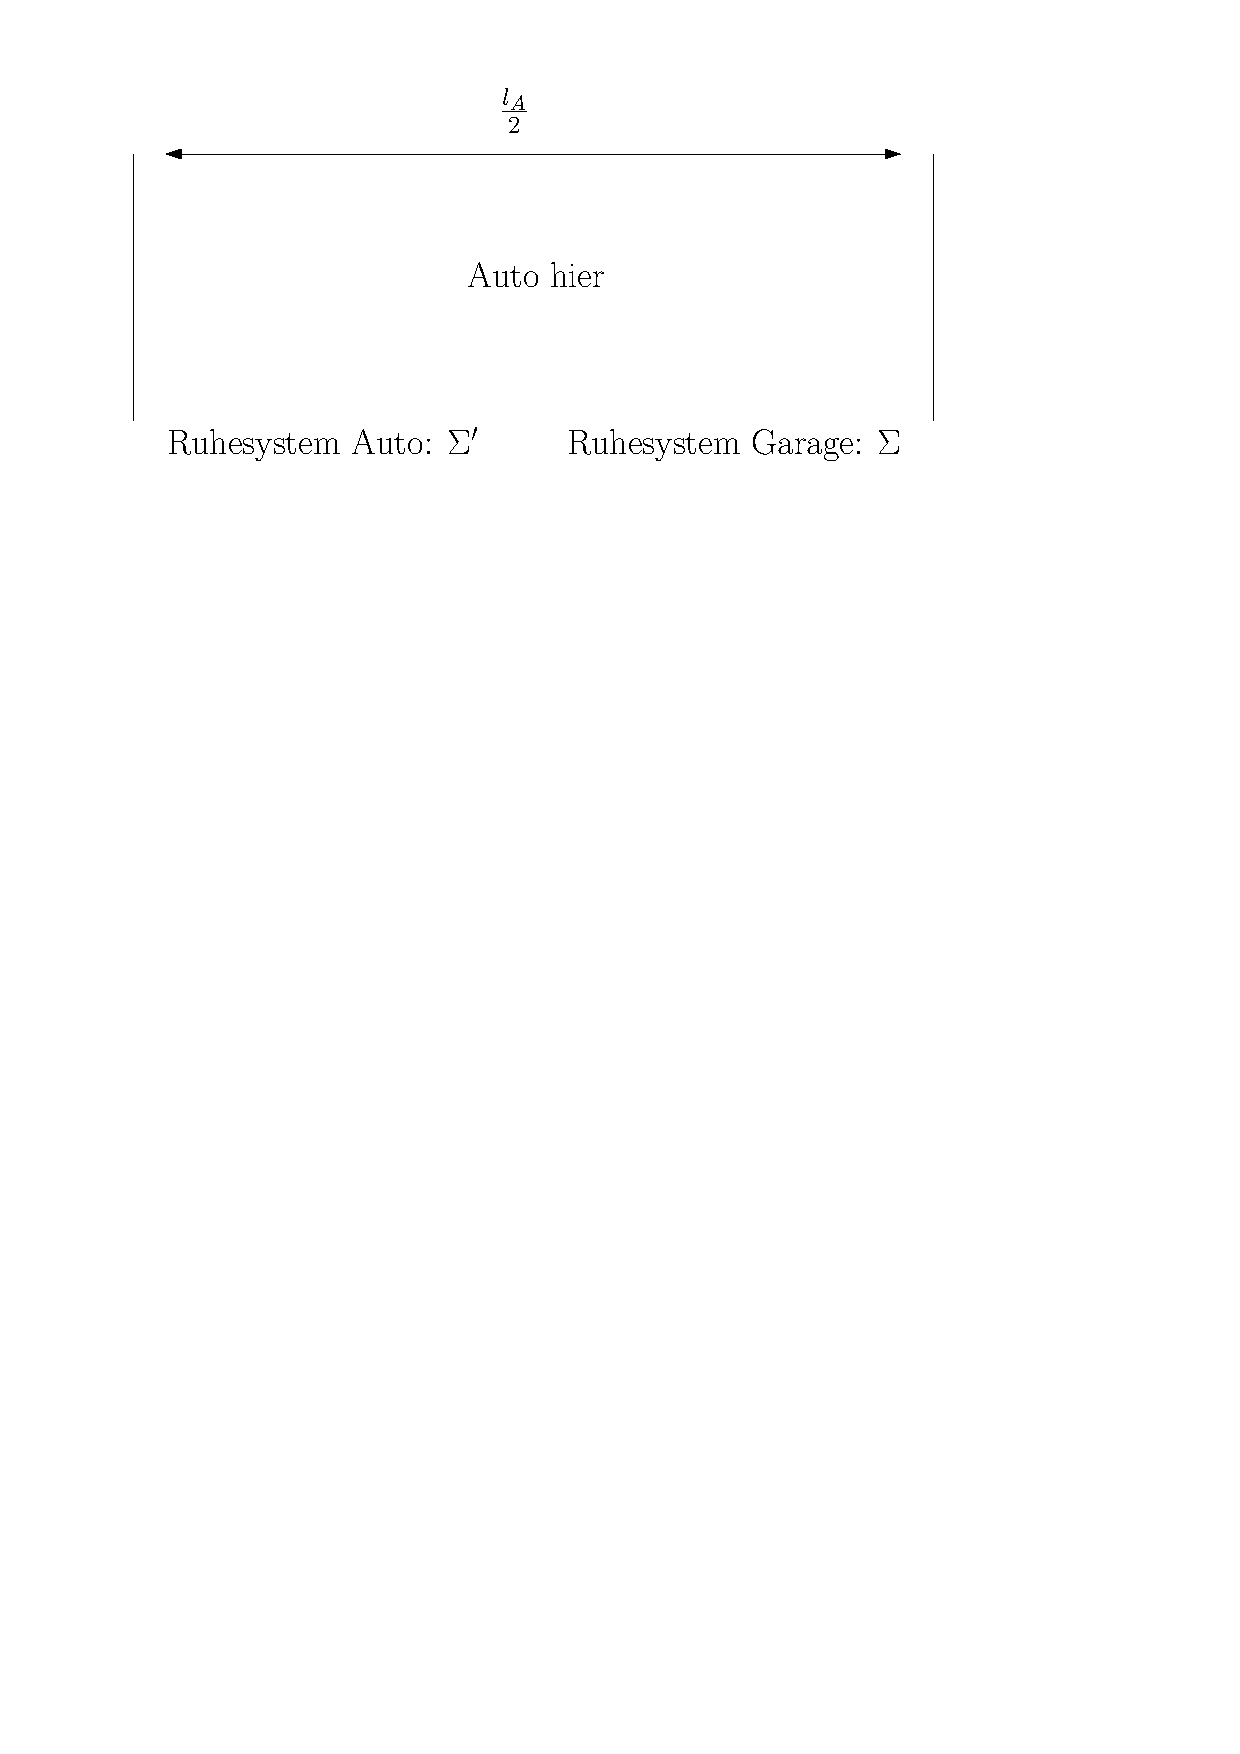
\includegraphics{figures/ueb11/aufgabe24}
	\caption{Aufgabe 24}
	\label{fig:ueb11_aufgabe24}
\end{figure}

Wir setzen $r = (ct, x, y, z)^T$, $r_0 = (c t_0, x_0 = 0)^T$ und $r_1 = (c t_1, x_1 = l_A)^T$ (im Ruhesystem $\Sigma$). Wichtig bei Längenmessung: Beide Endpunkten zum selben Zeitpunkt messen. Wie sieht $r$ in $\Sigma'$ aus? Ausrechnen:
\[
	r' = \Lambda(\vec{v}) r = \begin{pmatrix}
		\gamma & -\gamma \beta \\
		-\gamma \beta & \gamma
	\end{pmatrix}
	\mvec{ct \\ x}
	= \begin{pmatrix}
		\gamma (ct - \beta x) \\
		\gamma (-\beta ct + x)
	\end{pmatrix}
	\text{.}
\]
	
Wenn man das mit $r_0$ bzw. $r_1$ macht, führt das auf die Gleichungen
\[
	\left\{
	\begin{array}{l}
		c t'_0 = \gamma(ct_0 - \beta x_0) \\
		x'_0 = \gamma(-\beta c t_0 + x_0) 	
	\end{array}
	\right.
	\quad \text{ und } \quad
	\left\{
	\begin{array}{l}
		c t'_1 = \gamma(ct_1 - \beta x_1) \\
		x'_1 = \gamma(-\beta c t_1 + x_1) 	
	\end{array}
	\right.
	\text{.}
\]
	
Jetzt fordern wir $c t'_0 = c t'_1$ und damit $\gamma (ct_0 - \beta x_0) = \gamma (c t_1 - \beta x_1)$, also $c (t_1 - t_0) = \beta (x_1 - x_0)$. Es folgt 	
\begin{align*}
	l'_A &= x'_1 = x'_0 = \gamma (- \beta c (t_1 - t_0) + (x_1 - x_0))
	= \gamma (- \beta^2 (x_1 - x_0) + (x_1 - x_0)) \\
	&= \gamma \underbrace{(1 - \beta^2)}_{\frac{1}{\gamma^2}} l_A = \frac{1}{\gamma} l_A
	\text{.}
\end{align*}
Der Term wird als relativistische Längenkontraktion bezeichnet. Für die Aufgabe muss gelten: $\frac{l'_A}{l_A} = \sqrt{1 - \beta^2}$, also $\beta = \sqrt{1 - \left( \frac{l'_A}{l_A} \right)^2}$. Es folgt für $v$:
\[
	v = \sqrt{1 - \left( \frac{l'_A}{l_A} \right)^2} c = \sqrt{\frac{3}{4}} c = \frac{\sqrt{3}}{2} c
		\text{.}
\]

\section*{Aufgabe 25}

Myonen werden in $11 \si{km}$ Höhe erzeugt und haben eine Halbwertszeit $\tau_\mu = 2 \cdot 10^{-6} \si{s}$ und eine Geschwindigkeit von $v \approx c$.

Ohne relativistische Rechnung können sie also einen Weg $\Delta s = c \tau = 3 \cdot 10^5 \si{\frac{km}{s}} 2 \cdot 10^{-6} = 0.6 \si{km}$ zurücklegen und würden die Erdoberfläche somit nicht erreichen.

Nun relativistisch rechnen: System der Myonen sei $\Sigma$ und wir setzen $x_0 = (0, 0)^T$ und $x_1 = (c \tau, 0)^T$. System der Erde sei $\Sigma'$ und wir setzen analog $x'_0 = (0, h'_0)^T$ und $x'_1 = (ct, h'_1)^T$. 

Es ist
\[
	(x'_1 - x'_0) = \begin{pmatrix}
		\gamma & -\gamma \beta \\
		-\gamma \beta & \gamma
	\end{pmatrix}
	(x_1 - x_0)
	\text{,}
\]
also
\[
	\mvec{ct \\ h'_1 - h'_0} = \begin{pmatrix}
		\gamma & -\gamma \beta \\
		-\gamma \beta & \gamma
	\end{pmatrix}
	\mvec{c \tau \\ 0}
	\text{.}
\]
Für die Zeit gilt somit $ct = \gamma c \tau$. Das ist die Zeitdilatation: $t = \gamma \tau$ ($\gamma > 1$). Für die Höhe gilt:
\begin{align*}
	&~ h'_1 - h'_0 = - \gamma \beta c \tau \\
	\Longrightarrow &~ (h'_1 - h'_0)^2 = \frac{\beta^2}{1 - \beta^2} c^2 \tau^2 \\
	\Longleftrightarrow &~ (h'_1 - h'_0)^2 (1 - \beta^2) = \beta^2 c^2 \tau^2 \\
	\Longleftrightarrow &~ \beta^2 ((h'_1 - h'_0)^2 + c^2 \tau^2) = (h'_1 - h'_0)^2 \\
	\Longleftrightarrow &~ \beta^2 = \frac{(h'_1 - h'_0)^2}{(h'_1 - h'_0) + c^2 \tau^2} = \frac{1}{1 + \frac{c^2 \tau^2}{(h'_1 - h'_0)^2}} \\
	\Longrightarrow &~ \beta = \left( 1 + \frac{c^2 \tau^2}{(h'_1 - h'_0)^2} \right)^{- \frac{1}{2}}
	= \left( 1 + \frac{2 \cdot 10^{-6} s 3 \cdot 10^5 \si{\frac{km}{s}}}{(11 \si{km} - 1.5 \si{km})^2} \right)^{-\frac{1}{2}}
	\approx 0.998
	\text{.}
\end{align*}
	\chapter*{Übung 12}

\section*{Aufgabe 26}

Inertialsystem $\Sigma$ und Zeipunkt $t_0 = 0$: Beobachter $B$ und $B'$ an der selben Stelle. $B'$ bewegt sich mit $v$ von $B$ weg. Zum Zeitpunkt $t_1$ sind $B$ und $B'$ $\Delta s_1 = \Delta s_2$ voneinander entfernt und $B'$ dreht um. Zum Zeitpunkt $t_2$ sind $B$ und $B'$ wieder an der selben Position. 

Wir setzen $\Delta t_s = t_s - t_{s - 1}$. Es ist $\Delta s_1 = 15 \si{c \cdot a} = \Delta s_2$, $\Delta t_1 = 15 \si{a} \Delta t_2$ und $t_2 = 30 \text{ Jahre}$.

Gegeben ist, dass $v \approx c$, also $\beta = \frac{v}{c} \approx 1$ und somit $\gamma = \frac{1}{\sqrt{1 - \beta^2}} \rightarrow \infty$. Ist $\Delta t_1 = \frac{\Delta s_1}{v}$, dann ist mit Zeitdilatation\footnote{$t = \gamma \tau$} $\Delta t_1' = \frac{1}{\gamma} \Delta t_1$. Weiter ist $\Delta t_2 = \frac{\Delta s_2}{v} = \frac{\Delta s_1}{v}$ und $\Delta t_2' = \frac{1}{\gamma} \Delta t_1$. Da $t_2' = \Delta t_1' + \Delta t_2' = \frac{2 \Delta s_1}{\gamma v}$ folgt
$t_2' = \lim_{\gamma \rightarrow \infty} \frac{2 \Delta s_1}{\gamma v} = 0$.

Jetzt ist $v = \frac{c}{2}$, also $\beta = \frac{1}{2}$ und $\gamma = \frac{1}{\sqrt{1 - 1/4}} = \frac{2}{\sqrt{3}}$. Mit der Formel von eben folgt $t_2' = \frac{\sqrt{3}}{2} \frac{2 \Delta s}{\frac{c}{2}} \approx 52 \text{ Jahre}$.


Nun betrachte Skizze \ref{fig:ueb12_aufgabe26}.

\begin{figure}[h]
	\centering
	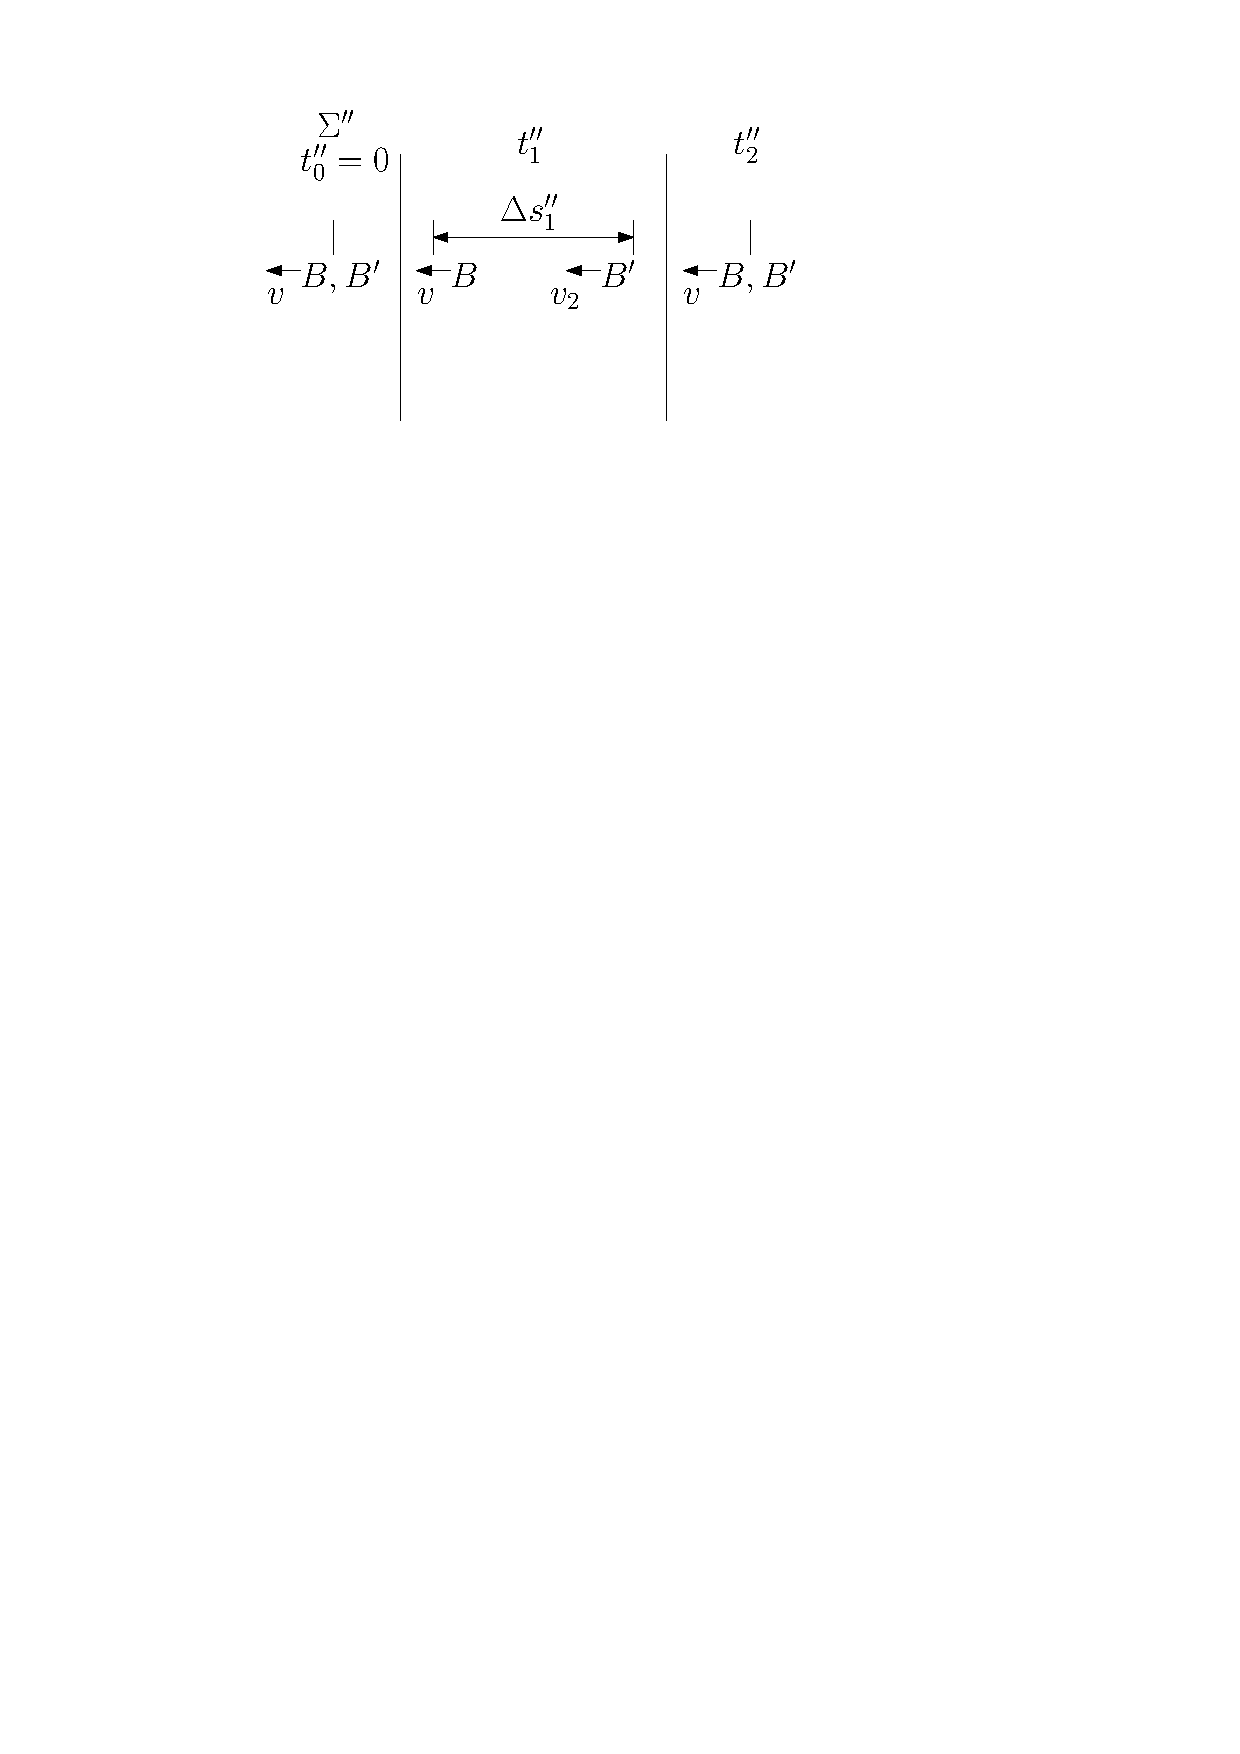
\includegraphics{figures/ueb12/aufgabe26}
	\caption{Aufgabe 26, c)}
	\label{fig:ueb12_aufgabe26}
\end{figure}

Es gilt $v_2 = \frac{v + v}{1 + \frac{v v}{c^2}} = \frac{2 v}{1 + \frac{v^2}{c^2}}$, $\beta_{v_2} = \frac{v_2}{c} = \frac{2 \beta}{1 + \beta^2}$ und 
\[
	\gamma_{v_2} = \frac{1}{\sqrt{1 - \beta^2_{v_2}}} = \frac{1}{\sqrt{1 - \frac{4 \beta^2}{(1 + \beta^2)^2}}} = \frac{1 + \beta^2}{\sqrt{(1 + \beta^2)^2 - 4 \beta^2}} 
	= \frac{1 + \beta^2}{\sqrt{(1 - \beta^2)^2}} = \frac{1 + \beta^2}{1 - \beta^2}
	\text{.}
\]

Erkenntnisse: 
\begin{enumerate}
	\item $\Delta t_1'' = \frac{1}{\gamma} \frac{\Delta s_1}{v} = \Delta t_1'$,
	\item $\Delta s_2'' = \Delta t_2'' \cdot v + \Delta s_1'' = \Delta t_2'' v_2$,
	\item $\Delta t_2'' v + \underbrace{\Delta s_1''}_{\Delta s_1 / \gamma} = \Delta t_2'' \frac{2 v}{1 + \beta^2} 
	~\Leftrightarrow~ 
	\Delta t_2'' v \left( \frac{2}{1 + \beta^2} - 1 \right) = \frac{\Delta s_1}{\gamma} 
	~\Leftrightarrow~
	\Delta t_2'' = \frac{\Delta s_1}{\gamma v} \left( \frac{2 - (1 + \beta^2)}{1 + \beta^2} \right)^{-1} = \frac{\Delta s_1}{\gamma v} \frac{1 + \beta^2}{1 - \beta^2}$,
	\item $\Delta t_2' = \frac{1}{\gamma v_2} \Delta t_2'' = \frac{1 - \beta^2}{1 + \beta^2} \frac{\Delta s_1}{\gamma v} \frac{1 + \beta^2}{1 - \beta^2} = \frac{\Delta s_1}{\gamma v}$ und schließlich
	\item $t_2' = \frac{2 \Delta s_1}{\gamma v}$.
\end{enumerate}
 
\section*{Aufgabe 27}

Eine Skizze ist auf dem Aufgabenblatt. 

\begin{description}
	\item[a)] Ein Teilchen in Ruhe mit $(m_0 c, 0, 0, 0)^T = (E / c, \vec{p})^T$ wird in $z$-Richtung geboostet:
	\[
		\begin{pmatrix}
			\gamma & - \beta \gamma & 0 & 0 \\
			- \beta \gamma & \gamma & 0 & 0 \\
			0 & 0 & 1 & 0 \\
			0 & 0 & 0 & 1
		\end{pmatrix}
		\mvec{m_0 c^2 \\ 0 \\ 0 \\ 0}
		= \mvec{\gamma m_0 c \\ - \beta \gamma m_0 c \\ 0 \\ 0} \text{,}
	\]
	also ist $E = mc^2 = \gamma m_0 c^2$. Die effektive Masse ist $m = \gamma m_0$.
	
	\item[b)] Die Energie-Impuls-Erhaltung schreibt man wie folgt auf (wobei $\vec{p}_e = \vec{0}$):
	\[
		\mvec{\frac{E_\gamma}{c} \\ \vec{p}_\gamma} + \mvec{\frac{E_e}{c} \\ \vec{p}_e}
		\overset{!}{=} \mvec{\frac{E_e'}{c} \\ \vec{p}\,'_e} + \mvec{\frac{E_\gamma'}{c} \\ \vec{p}\,'_\gamma} 
		\text{.}
	\]
	Also muss 
	\begin{enumerate}
		\item $p_\gamma + p_e = p'_\gamma + p'_e ~\Longrightarrow~ p'_e = p_\gamma + p_e - p'_\gamma$ und 
		\item $p^{'2}_e = p_\gamma^2 + p^{'2}_\gamma + p^{'2}_e + 2 (p_\gamma - p'_\gamma) p_e - 2 p_\gamma p'_\gamma$.
	\end{enumerate}
	
	Aus 2. folgt weiter 
	\begin{align*}
		& p^{'2}_\gamma = p^2_\gamma = 0 = \frac{E^2_\gamma}{c^2} - \mabs{\vec{p}_\gamma}^2 \\
		\Longleftrightarrow~& \vec{p}^2_\gamma = \frac{E^2_\gamma}{c^2} \text{,} \\
		& p^2_e = m^2_e c^2 = p^{'2}_e \text{,} \\
		& m^2_e c^2 = m_e^2 c^2 + 2(E_\gamma - E'_\gamma) E_e \frac{1}{c^2} - 2 (E_\gamma E'_\gamma \frac{1}{c^2} - \vec{p}_\gamma \vec{p}\,'_\gamma) \text{,} \\
		& \vec{p}_\gamma \vec{p}\,'_\gamma = \mabs{\vec{p}_\gamma} \mabs{\vec{p}\,'_\gamma} \cos \Theta_\gamma = \frac{E_\gamma E'_\gamma}{c^2} \cos \Theta_\gamma \\
		\Longleftrightarrow~& 0 = (E_\gamma - E'_\gamma) m_e c^2 - E_\gamma E'_\gamma (1 - \cos \Theta_\gamma) \\
		\Longleftrightarrow~& E'_\gamma (m_e c^2 + E_\gamma (1 - \cos \Theta_\gamma)) = E_\gamma m_e c^2 \\
		\Longleftrightarrow~& E'_\gamma = \frac{E_\gamma}{1 + \frac{E_\gamma}{m_e c^2} (1 - \cos \Theta_\gamma)} \text{.}
	\end{align*}

	\item[c)] Erinnerung: $E_\gamma = \frac{2 \pi \hbar c}{\lambda} = \frac{h c}{\lambda}$ und $\lambda = \frac{h}{\mabs{\vec{p}_\gamma}} = \frac{hc}{E_\gamma}$. Es ist 
	\begin{align*}
		& 0 = 2 \pi \hbar c \left( \frac{1}{\lambda} - \frac{1}{\lambda'} \right) - \frac{1 - \cos \Theta}{m_e c^2} (2 \pi \hbar)^2 \frac{1}{\lambda} \frac{1}{\lambda'} c^2 \\
		\Longleftrightarrow~& \Delta \lambda = \frac{2 \pi \hbar}{m_e c} \underbrace{(1 - \cos \Theta_\gamma)}_{2 \sin^2\left( \frac{\Theta}{2} \right)} \text{.}
	\end{align*}
\end{description}
\end{document}

%%% Local Variables:
%%% mode: latex
%%% TeX-master: t
%%% End:
